\documentclass[]{book}
\usepackage{lmodern}
\usepackage{amssymb,amsmath}
\usepackage{ifxetex,ifluatex}
\usepackage{fixltx2e} % provides \textsubscript
\ifnum 0\ifxetex 1\fi\ifluatex 1\fi=0 % if pdftex
  \usepackage[T1]{fontenc}
  \usepackage[utf8]{inputenc}
\else % if luatex or xelatex
  \ifxetex
    \usepackage{mathspec}
  \else
    \usepackage{fontspec}
  \fi
  \defaultfontfeatures{Ligatures=TeX,Scale=MatchLowercase}
\fi
% use upquote if available, for straight quotes in verbatim environments
\IfFileExists{upquote.sty}{\usepackage{upquote}}{}
% use microtype if available
\IfFileExists{microtype.sty}{%
\usepackage{microtype}
\UseMicrotypeSet[protrusion]{basicmath} % disable protrusion for tt fonts
}{}
\usepackage[margin=1in]{geometry}
\usepackage{hyperref}
\hypersetup{unicode=true,
            pdftitle={From my lovers and others. (Letters from 2013-2014)},
            pdfauthor={Carlos Alcala a.k.a. Carlito Fluito},
            pdfborder={0 0 0},
            breaklinks=true}
\urlstyle{same}  % don't use monospace font for urls
\usepackage{natbib}
\bibliographystyle{apalike}
\usepackage{longtable,booktabs}
\usepackage{graphicx,grffile}
\makeatletter
\def\maxwidth{\ifdim\Gin@nat@width>\linewidth\linewidth\else\Gin@nat@width\fi}
\def\maxheight{\ifdim\Gin@nat@height>\textheight\textheight\else\Gin@nat@height\fi}
\makeatother
% Scale images if necessary, so that they will not overflow the page
% margins by default, and it is still possible to overwrite the defaults
% using explicit options in \includegraphics[width, height, ...]{}
\setkeys{Gin}{width=\maxwidth,height=\maxheight,keepaspectratio}
\usepackage[normalem]{ulem}
% avoid problems with \sout in headers with hyperref:
\pdfstringdefDisableCommands{\renewcommand{\sout}{}}
\IfFileExists{parskip.sty}{%
\usepackage{parskip}
}{% else
\setlength{\parindent}{0pt}
\setlength{\parskip}{6pt plus 2pt minus 1pt}
}
\setlength{\emergencystretch}{3em}  % prevent overfull lines
\providecommand{\tightlist}{%
  \setlength{\itemsep}{0pt}\setlength{\parskip}{0pt}}
\setcounter{secnumdepth}{5}
% Redefines (sub)paragraphs to behave more like sections
\ifx\paragraph\undefined\else
\let\oldparagraph\paragraph
\renewcommand{\paragraph}[1]{\oldparagraph{#1}\mbox{}}
\fi
\ifx\subparagraph\undefined\else
\let\oldsubparagraph\subparagraph
\renewcommand{\subparagraph}[1]{\oldsubparagraph{#1}\mbox{}}
\fi

%%% Use protect on footnotes to avoid problems with footnotes in titles
\let\rmarkdownfootnote\footnote%
\def\footnote{\protect\rmarkdownfootnote}

%%% Change title format to be more compact
\usepackage{titling}

% Create subtitle command for use in maketitle
\newcommand{\subtitle}[1]{
  \posttitle{
    \begin{center}\large#1\end{center}
    }
}

\setlength{\droptitle}{-2em}

  \title{From my lovers and others. (Letters from 2013-2014)}
    \pretitle{\vspace{\droptitle}\centering\huge}
  \posttitle{\par}
    \author{Carlos Alcala a.k.a. \href{www.carlitofluitoideas.com}{Carlito Fluito}}
    \preauthor{\centering\large\emph}
  \postauthor{\par}
      \predate{\centering\large\emph}
  \postdate{\par}
    \date{2020-04-24}

\usepackage{booktabs}

\begin{document}
\maketitle

{
\setcounter{tocdepth}{1}
\tableofcontents
}
\hypertarget{preamble}{%
\chapter*{Preamble}\label{preamble}}
\addcontentsline{toc}{chapter}{Preamble}

We are socially fragmented.

Memory, knowledge, lives, even identities. Everything is dispersed (another argument supporting the non-local consciousness theory).

The aim of this epistolary work is to know a bit better what I am now thorugh the compilation of pieces of what I have been. I have been told in the past that there was wisdom in the texts I wrote, and I am sure that there is wisdom in the texts I received.

I hope you find something that makes your life more meaningful and satisfactory. I hope you find a bunch of human beings that, like you, have suffered and have enjoyed moments of their lives. A bunch of human beings that, after all, have lived.

\hypertarget{intro}{%
\subsection*{If you don't know me\ldots{}}\label{intro}}
\addcontentsline{toc}{subsection}{If you don't know me\ldots{}}

If this is the first time you find out about me, I am Carlos Alcala a.k.a. Carlito Fluito. I like sharing my ideas and experiences through \href{www.carlitofluitoideas.com}{writing}, \href{www.carlitofluito.com}{performing}, sporadic \href{https://www.youtube.com/channel/UC5Q8igPq_lE1JQNwbjjy7wA}{YouTube videos}, and spontaneous \href{https://www.instagram.com/carlitofluito/?hl=en}{Instagram posts}.

\begin{figure}

{\centering 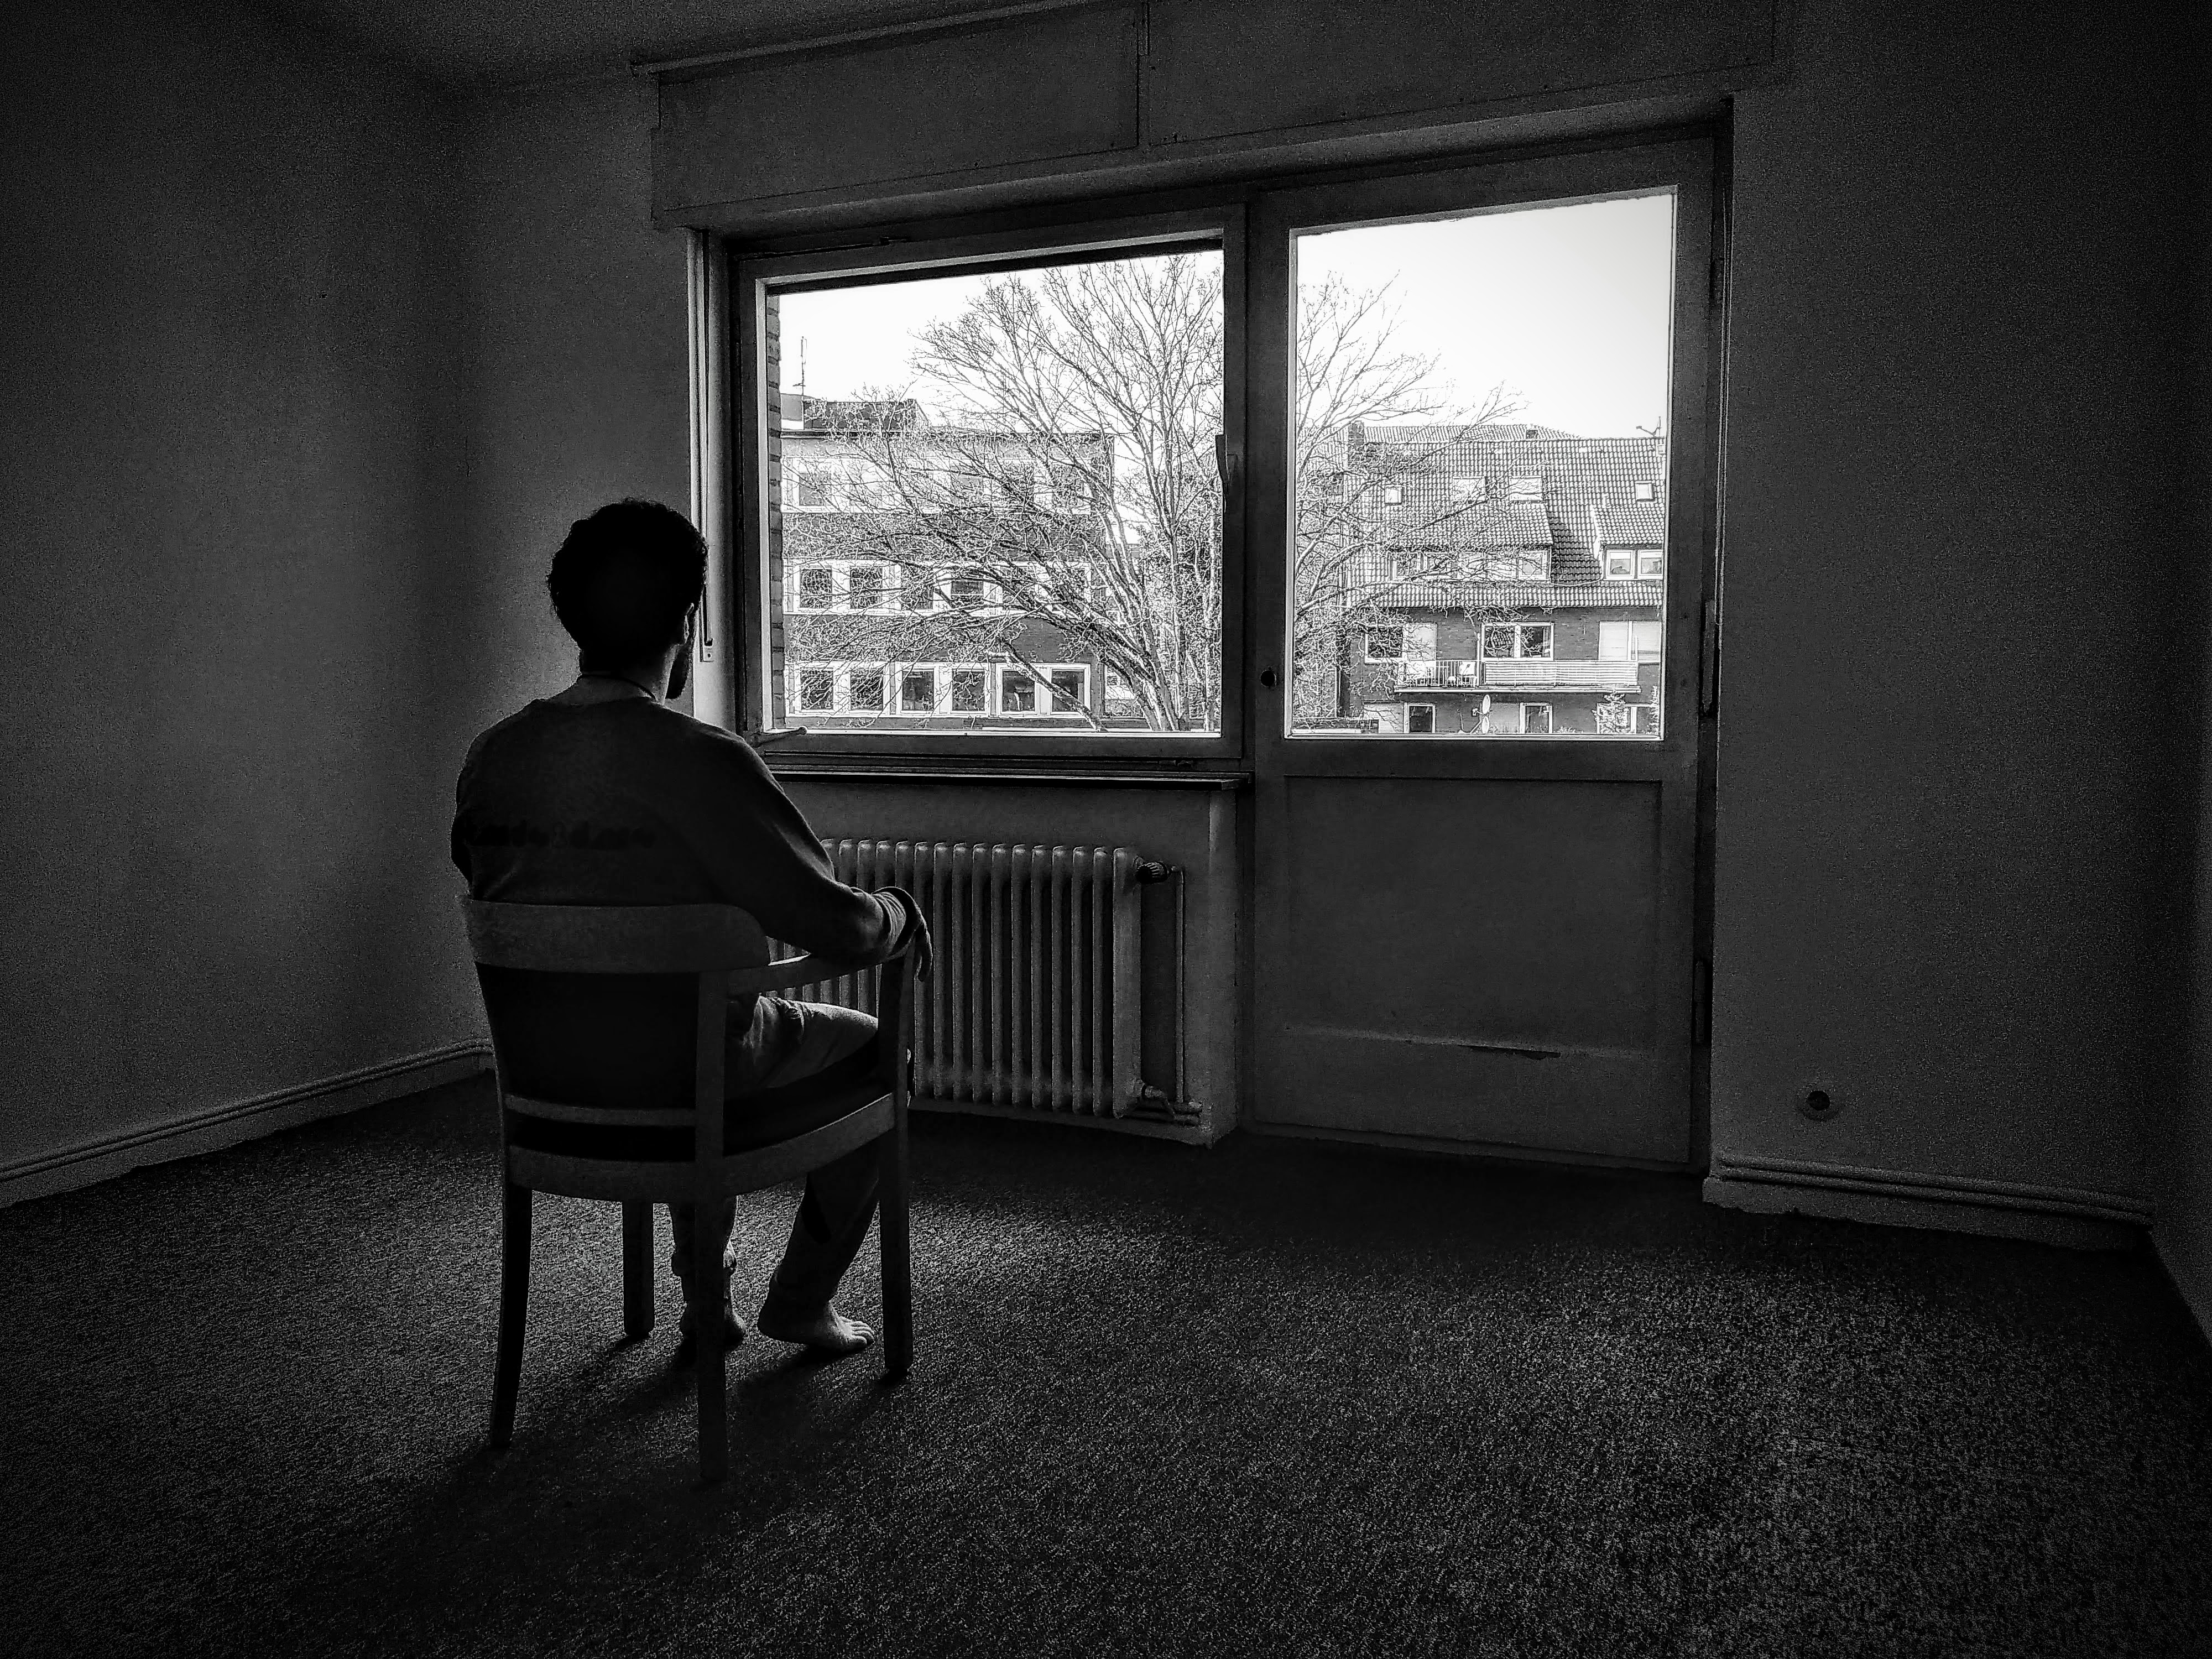
\includegraphics[width=0.75\linewidth]{images/2014/intro} 

}

\caption{ *Munster (Germany). March, 2020*: It took me a while to take this picture with my [Fairphone](https://www.fairphone.com/en/) and an improvised tripod. I like the result, though.}\label{fig:intro}
\end{figure}

The seriousness of my content varies from ``\emph{This guy is crazy!}'' to ``\emph{It makes sense what he's saying\ldots{}}''. In any case, As any other human being, I have needs to survive. If you find value in anything I do, and you want to keep me alive\footnote{Or help me growing, let's not be so dramatic.}, I will be extremelly grateful if you support me on \href{https://www.patreon.com/carlitofluito}{Patreon}\footnote{I am also a qualified psychologist, running online counseling and coaching sessions. Feel free to contact if you are interested in working together.}, or drop me a ``\emph{Thanks for creating}'' message.

Best, and enjoy reading!!

\hypertarget{context}{%
\section*{A bit of context}\label{context}}
\addcontentsline{toc}{section}{A bit of context}

In September 2013, I moved to Leuven (Belgium) to study my fourth and last year of Bachelor in Psychology. Many people warned me about the dangers of getting lost in the wild parties of the city, and how much a year as Erasmus student could teach me about the world. However, no one warned me about the perils I would encounter, or about how one given evening could actually change my whole life, being, and spirit\ldots{}

\begin{figure}

{\centering 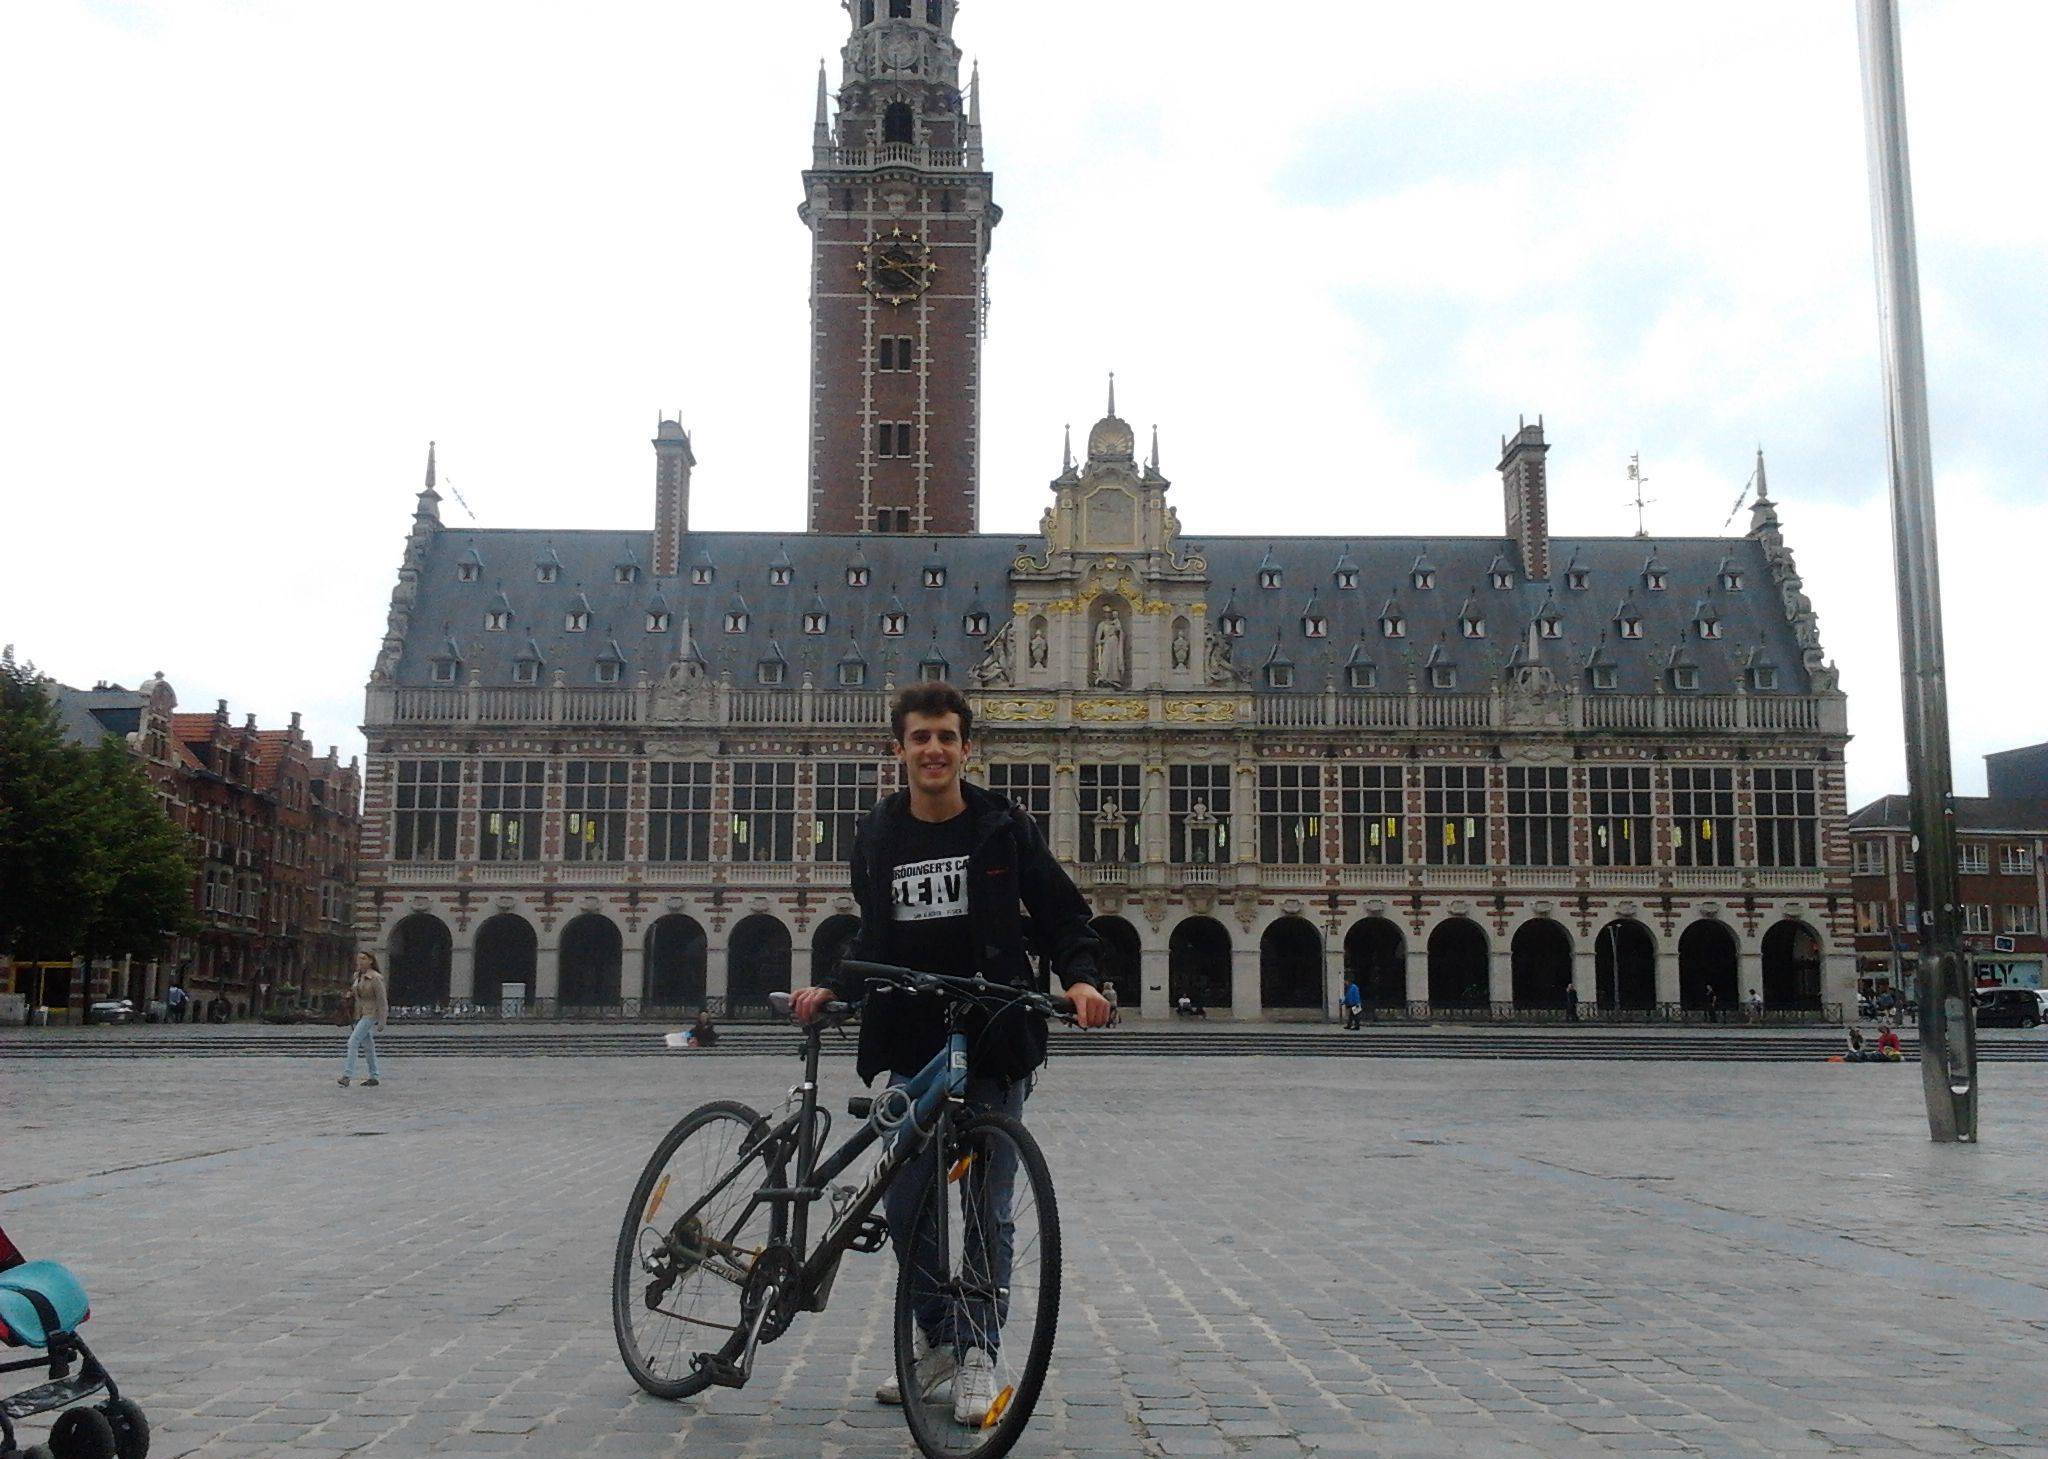
\includegraphics[width=0.75\linewidth]{images/2014/library} 

}

\caption{ *Leuven (Belgium). July, 2013*: Before the course started, I went to Leuven to find a place to live during the year. Not only, I found the room, but also a nice bike that still waits for me when I go to Valladolid (Spain). This is the triumphant hunting picture with the prize.}\label{fig:library}
\end{figure}

\hypertarget{arrival}{%
\chapter*{Arrival (September)}\label{arrival}}
\addcontentsline{toc}{chapter}{Arrival (September)}

These are mostly a compilation of the entries of the first (traveling) blog I made, \href{http://excusasparanovolver.blogspot.com/}{\emph{Excusas para no Volver}}\footnote{\emph{Excuses for not coming back}. Not coming back to my home country? Not coming back to the visited country? }. I hadn't started writing letters yet, just some spare emails that reflected of my situation. I used to do some online courses; exchange information and links with my friends T. (a philosopher), and F. (a poet); and all those things last year weird university students do.

They may not be so relevant nowadays, but I still think that it adds some layer of clarity over the person that I used to be and my evolution as a writer.

\hypertarget{fromtoF20130904}{%
\section*{2013-09-04 From and to F.}\label{fromtoF20130904}}
\addcontentsline{toc}{section}{2013-09-04 From and to F.}

Little fagot things\ldots{}

\href{https://en.wikipedia.org/wiki/Kseniya_Ryzhova\#2013_Moscow_kiss}{Russian athletes} first, \href{http://www.elmundo.es/elmundo/2013/09/03/gentes/1378227703.html}{now} \href{https://en.wikipedia.org/wiki/Alain_Delon}{Delon}. France and Russia are resisting They believed in the Revolution, which is a serious thing, and that is why he faces these little fagot things. Let's see if we lose the fear of what correctness. If homosexuals want to exist, they exist, what are they going to do. But do not tell us that it's normal. The most extended neither, of course not. And in favor of nature, of course neither do they go.

\begin{enumerate}
\def\labelenumi{\Alph{enumi}.}
\setcounter{enumi}{5}
\item
\end{enumerate}

\begin{center}\rule{0.5\linewidth}{\linethickness}\end{center}

Cats didn't purr? I only see scratches and bites around here \ldots{}

F., analysis, analysis!!!!

I will only make statements:

\begin{enumerate}
\def\labelenumi{\arabic{enumi}.}
\item
  Origin of homosexuality. Mainly, it is believed to have a \href{https://en.wikipedia.org/wiki/Homosexuality\#Causes}{genetic origin}. Then it is no longer so against nature, since it's nature that creates it spontaneously. In fact, in \href{https://en.wikipedia.org/wiki/Homosexuality\#Homosexual_behavior_in_other_animals}{other species there is homosexuality}, but only in the human species is \href{https://en.wikipedia.org/wiki/Homophobia}{homophobia}.
\item
  While it is true that it is not something that brings new offspring to the species, as human beings, they must be respected, and offensive comments such as ``unnatural'' is not respect. Furthermore, the bad thing about these comments is not the words, but the attitudes and the possible consequences and repercussions that these may have in this social sector.
\item
  The creation of a \href{https://en.wikipedia.org/wiki/Russian_gay_propaganda_law}{law against homosexual propaganda} is a restriction of a right and freedom that is not harmful to the population, and that causes negative discrimination in these citizens.
\item
  Although it is not the ``normal'' or the most widespread tendency, homosexuals are human beings in the same way as the others, and they must be treated as such. I know many homosexuals who are beautiful people, and they have taught me to love (love is a very big word, you know) men more even than women, but in a different ways.
\end{enumerate}

And as a typical and topical example, \href{https://en.wikipedia.org/wiki/Homosexuality\#Classical_period}{homosexuality practiced by the Greeks of Classical Greece}, the cradle of some of the greatest thinkers in the West.

F., do not take the email as an attack on your ideas, I like that you share this information with me, because they connect me with a reality and a society with which I often disconnect. But what I am going to like the most is what T. will answer, and the probable article in \href{http://ultimocero.com/}{Último Cero} that he is going to write.

With love from man to man,

Carlos, The goody-goody.

\begin{center}\rule{0.5\linewidth}{\linethickness}\end{center}

Carlos,

\begin{enumerate}
\def\labelenumi{\arabic{enumi}.}
\item
  Nature also creates cancers.
\item
  Everyone must be respected. Against nature is equivalent to say that it is not in favor of sustaining the world, it is not in favor of evolution, of conception. Let's take a radical example: tomorrow we all become homosexual. The Earth, after a few years, as long as science doesn't give up creating little children out of nothing, would become extinct. But they are few and we can continue to manage.
\item
  I notice a gay fashion. I'm not uncomfortable with others taking out a banner against it. I enjoy.
\item
  I also know excellent homosexuals.
\item
  Homosexuality in Greece was above all vice, pleasure, sex, desire. Here, it is presented equated to heterosexuality.
\end{enumerate}

Howls.

\begin{center}\rule{0.5\linewidth}{\linethickness}\end{center}

C., with whom in the end you are going to have a lot in common, uses a term that we make us laugh. ``\emph{Tree}'', he calls a large number of people: \emph{trees}. People without curiosity, with little motivation. Trees like to take root. You water them from time to time, they get the sun, they do photosynthesis and they live so happy wherever you plant them.

He believes that the danger is in the trees, and not in technology or science. It is the trees that are dangerous, those that can misinterpret ideas, and unleash terrible acts. I do not believe in goody-goody philosophies, because I know the enormous human stupidity. That is the real danger of radical and extremist ideas, and more so when they go against a sector of the population.

I am not so scared or too disturbed about educated people with the capacity to defend ideas I don't share about homosexuality, politics, etc.. It disturbs me more how trees can interpret these ideas. Worst of all, trees here are not fixed to the ground by roots. Their branches have access to a technology that can be very harmful \ldots{}

Purrs

PS: I have \href{https://en.wikipedia.org/wiki/Old_Possum\%27s_Book_of_Practical_Cats}{\emph{Old Possum's Book of Practical Cats}} at home \citep{eliot2014old}. I bought it in London last year. You live less than two minutes distance by bike, and 5 walking. Don't force me to bring it to you.

\begin{center}\rule{0.5\linewidth}{\linethickness}\end{center}

\begin{quote}
I begin this review with the famous, and polemical, declaration by T. S. Eliot. Although it is only some sixty-seven years since he published, in 1948, his essay Notes Towards the Definition of Culture, when we reread it today, it seems to refer to a very remote era, without any connection to the present.

T. S. Eliot assures us that his aim is merely to help define the concept of culture, but, in fact, his ambition is much greater, for, as well as specifying what the term means, he offers a penetrating criticism of the cultural system of his time, which, according to him, is becoming ever more distant from the ideal model that it represented in the past. In a sentence that might have appeared excessive at the time of writing, he argues, `I see no reason why the decay of culture should not proceed much further, and why we may not even anticipate a period, of some duration, of which it will be possible to say that it will have no culture.'1 (Anticipating my argument in Notes on the Death of Culture, I will say that the period Eliot is referring to is the one in which we are now living.)

That ideal older model, according to Eliot, is a culture made up of three `senses' of the term: the individual, the group or class, and the whole society. While there is some interaction between these three areas, each maintains a certain autonomy and develops in a state of constant tension with the others, within an order that allows the whole of society to prosper and maintain its cohesiveness.

T. S. Eliot states that what he calls `higher culture' is the domain of an elite, and he justifies this by asserting that `it is an essential condition of the preservation of the quality of the culture of a minority, that it should continue to be a minority culture' (p.~107). Like the elite, social class is also a reality that must be maintained, because the caste or group that guarantees higher culture is drawn from these ranks, an elite that should not be completely identified with the privileged group or aristocracy from which most of its members are drawn. Each class has the culture that it produces and that is appropriate to it and although, naturally, these cultures coexist, there are also marked differences that have to do with the economic conditions of each. One cannot conceive of an identical aristocratic and rural culture, for example, even though both classes share many things, such as religion and language.

Eliot's idea of class is not rigid or impermeable; rather it is open. A person from one class can move up or down a class, and it is good that this happens, even though it is an exception rather than the rule. This system both guarantees and expresses a social order, but today this order is fractured, which creates uncertainty about the future. The naive idea that, through education, one can transmit culture to all of society is destroying `higher culture', because the only way of achieving this universal democratization of culture is by impoverishing culture, making it ever more superficial. Just as the elite is indispensable to Eliot's conception of `higher culture', so also it is fundamental that a society has regional cultures that both nurture national culture and also exist in their own right with a certain degree of independence. `It is important that a man should feel himself to be not merely a citizen of a particular nation, but a citizen of a particular part of his country, with local loyalties. These, like loyalty to class, arise out of loyalty to the family' (p.~52).
\end{quote}

\begin{center}\rule{0.5\linewidth}{\linethickness}\end{center}

\emph{Notes on the Death of Culture} -- Vargas LLosa \citep{llosa2015notes}

Noted.

Forceful low hitting\ldots{} I guess that you'll have an unfinished and unfinishable list.

Still, it may be that current times are not the right path, but the past wasn't either.

Think of T.'s father. Let's believe (1\textsuperscript{st} plural from of the imperative of believe, not recognized in the \href{https://en.wikipedia.org/wiki/Royal_Spanish_Academy}{RSA} dictionary\footnote{Spanish nuance: \emph{Creamos} can be the imperative form of \emph{creer} {[}Let's believe{]} or present of \emph{crear} {[}We create{]} }) in opportunities. (Goody-goody striking back\ldots)

\begin{center}\rule{0.5\linewidth}{\linethickness}\end{center}

You have protection, so hits don't hurt. Well seen the title. A title that I have praised as much as criticized. I retire with the angels, who will not visit me tonight.

\begin{center}\rule{0.5\linewidth}{\linethickness}\end{center}

Good evening, and do not underestimate the help of Google (internet, science, technology, society, collaboration, cooperation, community, trees that write empty things in blogs \ldots), nor overestimate my ability.

I will give your address to the angels, to see if in this way\ldots{}

\hypertarget{toF20130908}{%
\section*{2013-09-08 To and from F}\label{toF20130908}}
\addcontentsline{toc}{section}{2013-09-08 To and from F}

Hi F.

I think I sent it in your period of not responding emails. Let me know what you think about it.

Salud,

Carlos

\begin{quote}
I'm late for my name

next to your name

and to the perfect silence of all gazes,

to the tireless night of adolescents.

I'm late for your dance

with bare legs,

to the fragile memory of small events,

to all the words you left in my belly.

I'm late for your face

so shy and perfect

and to the infinite beach with your body stretched out.

I'm late for the space

that was waiting in your bed,

to the kiss on the cheek

with sleeping eyes,

to my hand in your winter.

I'm late to write you

and love you slowly,

without doubts and without temples,

without counting the kisses.
\end{quote}

Original:

\begin{quote}
Llego tarde a mi nombre

al lado de tu nombre

y al silencio perfecto de todas las miradas,

a la noche incansable de los adolescentes.

Llego tarde a tu baile

con las piernas desnudas,

a la memoria frágil de los hechos pequeños,

a todas las palabras que dejaste en mi vientre.

Llego tarde a tu rostro

tan tímido y perfecto

y a la playa infinita con tu cuerpo tendido.

Llego tarde al espacio

que esperaba en tu cama,

al beso en la mejilla

con los ojos dormidos,

a mi mano en tu invierno.

Llego tarde a escribirte

y a quererte despacio,

sin dudas y sin templos,

sin contarnos los besos.

\citep{miralpeix2005cuerpo}
\end{quote}

\begin{center}\rule{0.5\linewidth}{\linethickness}\end{center}

Carlos,

Frankly good. It reminds me, based on my readings, aspects admired in \href{https://es.wikipedia.org/wiki/F\%C3\%A9lix_Grande}{Felix Grande} and \href{https://en.wikipedia.org/wiki/Jos\%C3\%A9_Manuel_Caballero}{Caballero Bonald}. Frankly good. Just the title -or first verse- is already worth the poem.

\begin{enumerate}
\def\labelenumi{\Alph{enumi}.}
\setcounter{enumi}{5}
\item
\end{enumerate}

\begin{center}\rule{0.5\linewidth}{\linethickness}\end{center}

Hi F.

\href{http://www.ccoo.cat/barcelones/documentacio/pdf_diversos/llibre_premi_Valverde_2011.pdf}{Page 35}

The poem chose me, it was the day, the place, and the moment \ldots{} You know that I only detect and sense ;)

Enjoy the second prize.

Carlos

\hypertarget{Excusas20130909}{%
\section*{\texorpdfstring{2013-09-09 Light subterfuges\footnote{First entry of \href{https://excusasparanovolver.blogspot.com/2013/09/subterfugios-de-luz.html}{\emph{Excusas para no volver}}, my first travelling blog.}}{2013-09-09 Light subterfuges}}\label{Excusas20130909}}
\addcontentsline{toc}{section}{2013-09-09 Light subterfuges}

Surprisingly, \href{https://en.wikipedia.org/wiki/Ryanair}{Ryanair} has arrived 35 minutes early. \href{https://en.wikipedia.org/wiki/Madrid}{Madrid}-\href{https://en.wikipedia.org/wiki/Charleroi}{Charleroi}, (1,500 km.) From 6.30 to 8.30. Low-Cost begins its economization with our most vital and valuable resource. There are no limits to savings. If the delays are cumulative, the advances as well. Dozens of passengers may have missed the flight today because the plane was taking off too soon. In sports competitions, it's advisable to keep the advantage. At 18:00 a plane with more than 9,000 kilometers in less than 12 hours begins to arrive late. The rush produces stumbles. Passengers, queues and impatience. Every river returns to its channel.

The cheapest way to get to Brussels from Charleroi (let no one fool you) is to take the buses from the Walloon area of Belgium, the \href{https://www.infotec.be/}{TEC company} to Charleroi Sud Gare. The buses are at the end of the terminal, you should not leave the terminal directly, but walk towards the end and there we find the vending machines. 5€ per person {[}CHARLEROI Brussel South Charleroi Airport GOSSELIES (HAINAUT) - CHARLEROI Sud Gare SNCB CHARLEROI (HAINAUT){]}. Later, at the South Station, if we are students under 26, we will buy a \href{https://www.belgiantrain.be/en}{GoPass (50€ for 10 trips) and if we are over 26 a RailPass (a bit more than 70€ for 10 trips)} This way we will get to Brussels for 10€ or 12€ depending on our age. Exquisite punctuality. At the airport we will find taxi drivers who offer the Charleroi-Brussels trip for 13€. A small price difference saves time. To the taste of the consumer.

The customer service of the Belgian train service officials is excellent. Many speak Spanish, in addition to English, French and Dutch (depending on the area); and they have no problem in providing you with a sheet of paper with the itinerary you have to follow to reach your destination. In our case, \href{https://en.wikipedia.org/wiki/Leuven}{Leuven}.

Once in Leuven, we have been surprised by blocked streets and a slight buzz of partying. Arriving at \href{https://en.wikipedia.org/wiki/Grote_Markt_(Leuven)}{Grote Markt} from the train station, along the Bondgenotenlaan (Avenue of the Allies), we find a picturesque scene. A bunch of Belgians, some of them independentists and a kind of parade starting at the town hall (Grote Markt). After having toured the city, a group of international students have come to Sint-Donatuspark to see a firework show. Just something to talk about. Forced introductions that will end in eternal farewells. I do not know the reasons for both, the congregation in Grote Markt and the fires in the park. I should continue investigating. I will not comment on the quality of the show, my Valencian friends would get angry.

I prefer symbolism.

The sky, black, burning and bleeding. No recoils are conceived; now they are tears. Artificial light that forcing the frowning. My face hurts. Squeaking in the calm of nature. That dark peace. Loud applause after twenty minutes of firecrackers. As a way of inauguration of my new life in this country, Belgium. Of my new life in this city, Leuven.

Now a real poem.

\begin{quote}
Light subterfuges, lizards, list

on top of the palm that creates it,

invention of colors in sight,

if transitory, blue, piraeus.

To the greater glory of the powdermaker,

straight the cane, circles plans:

a whole fleeting course of geometry,

beginning of its end, closed to the day.
\end{quote}

Original

\begin{quote}
Subterfugios de luz, lagartos, lista

encima de la palma que la crea,

invención de colores a la vista,

si transitoria, de azul, pirea.

A la gloria mayor del polvorista,

rectas la caña, círculos planea:

todo un curso fugaz de geometría,

principio de su fin, vedado al día.

\citet{hernandez1976perito}
\end{quote}

\hypertarget{toF20130911}{%
\section*{2013-09-11 To and from F}\label{toF20130911}}
\addcontentsline{toc}{section}{2013-09-11 To and from F}

Hello Carlos,

I'm going to tell you a story. Since years I've been chasing a discontinued book from \href{https://en.wikipedia.org/wiki/Julio_Llamazares}{Julio Llamazares}. He started writing poetry. He dried up. He made novel. He has not republished it for the respect it deserves. No verses come out. I had a photocopy of ``\emph{The slowness of the oxen}'' \citep{llamazares1985lentitud} and I was waiting to find it one way or another. \href{https://www.iberlibro.com/}{\emph{Iberlibro}} has brought me closer to no less than the 1975 original edition. Write that one down in favor of suicide technology.

By the way, I acquired the first reissue, from 1985 in \href{https://www.hiperion.com/}{``\emph{Hiperión}''}, which was also there. A certain José González, allegedly in love with a certain Sara, bought it on \href{https://en.wikipedia.org/wiki/Gran_V\%C3\%ADa,_Madrid}{Gran Vía} and gave it to her, surely wanting to tell her through those poisonous pages so many things. He dated it as ``\emph{7-X-85}'' with the decryption `\emph{opos-agricultural'85-}'. Maybe she had abandoned him.

\begin{figure}

{\centering 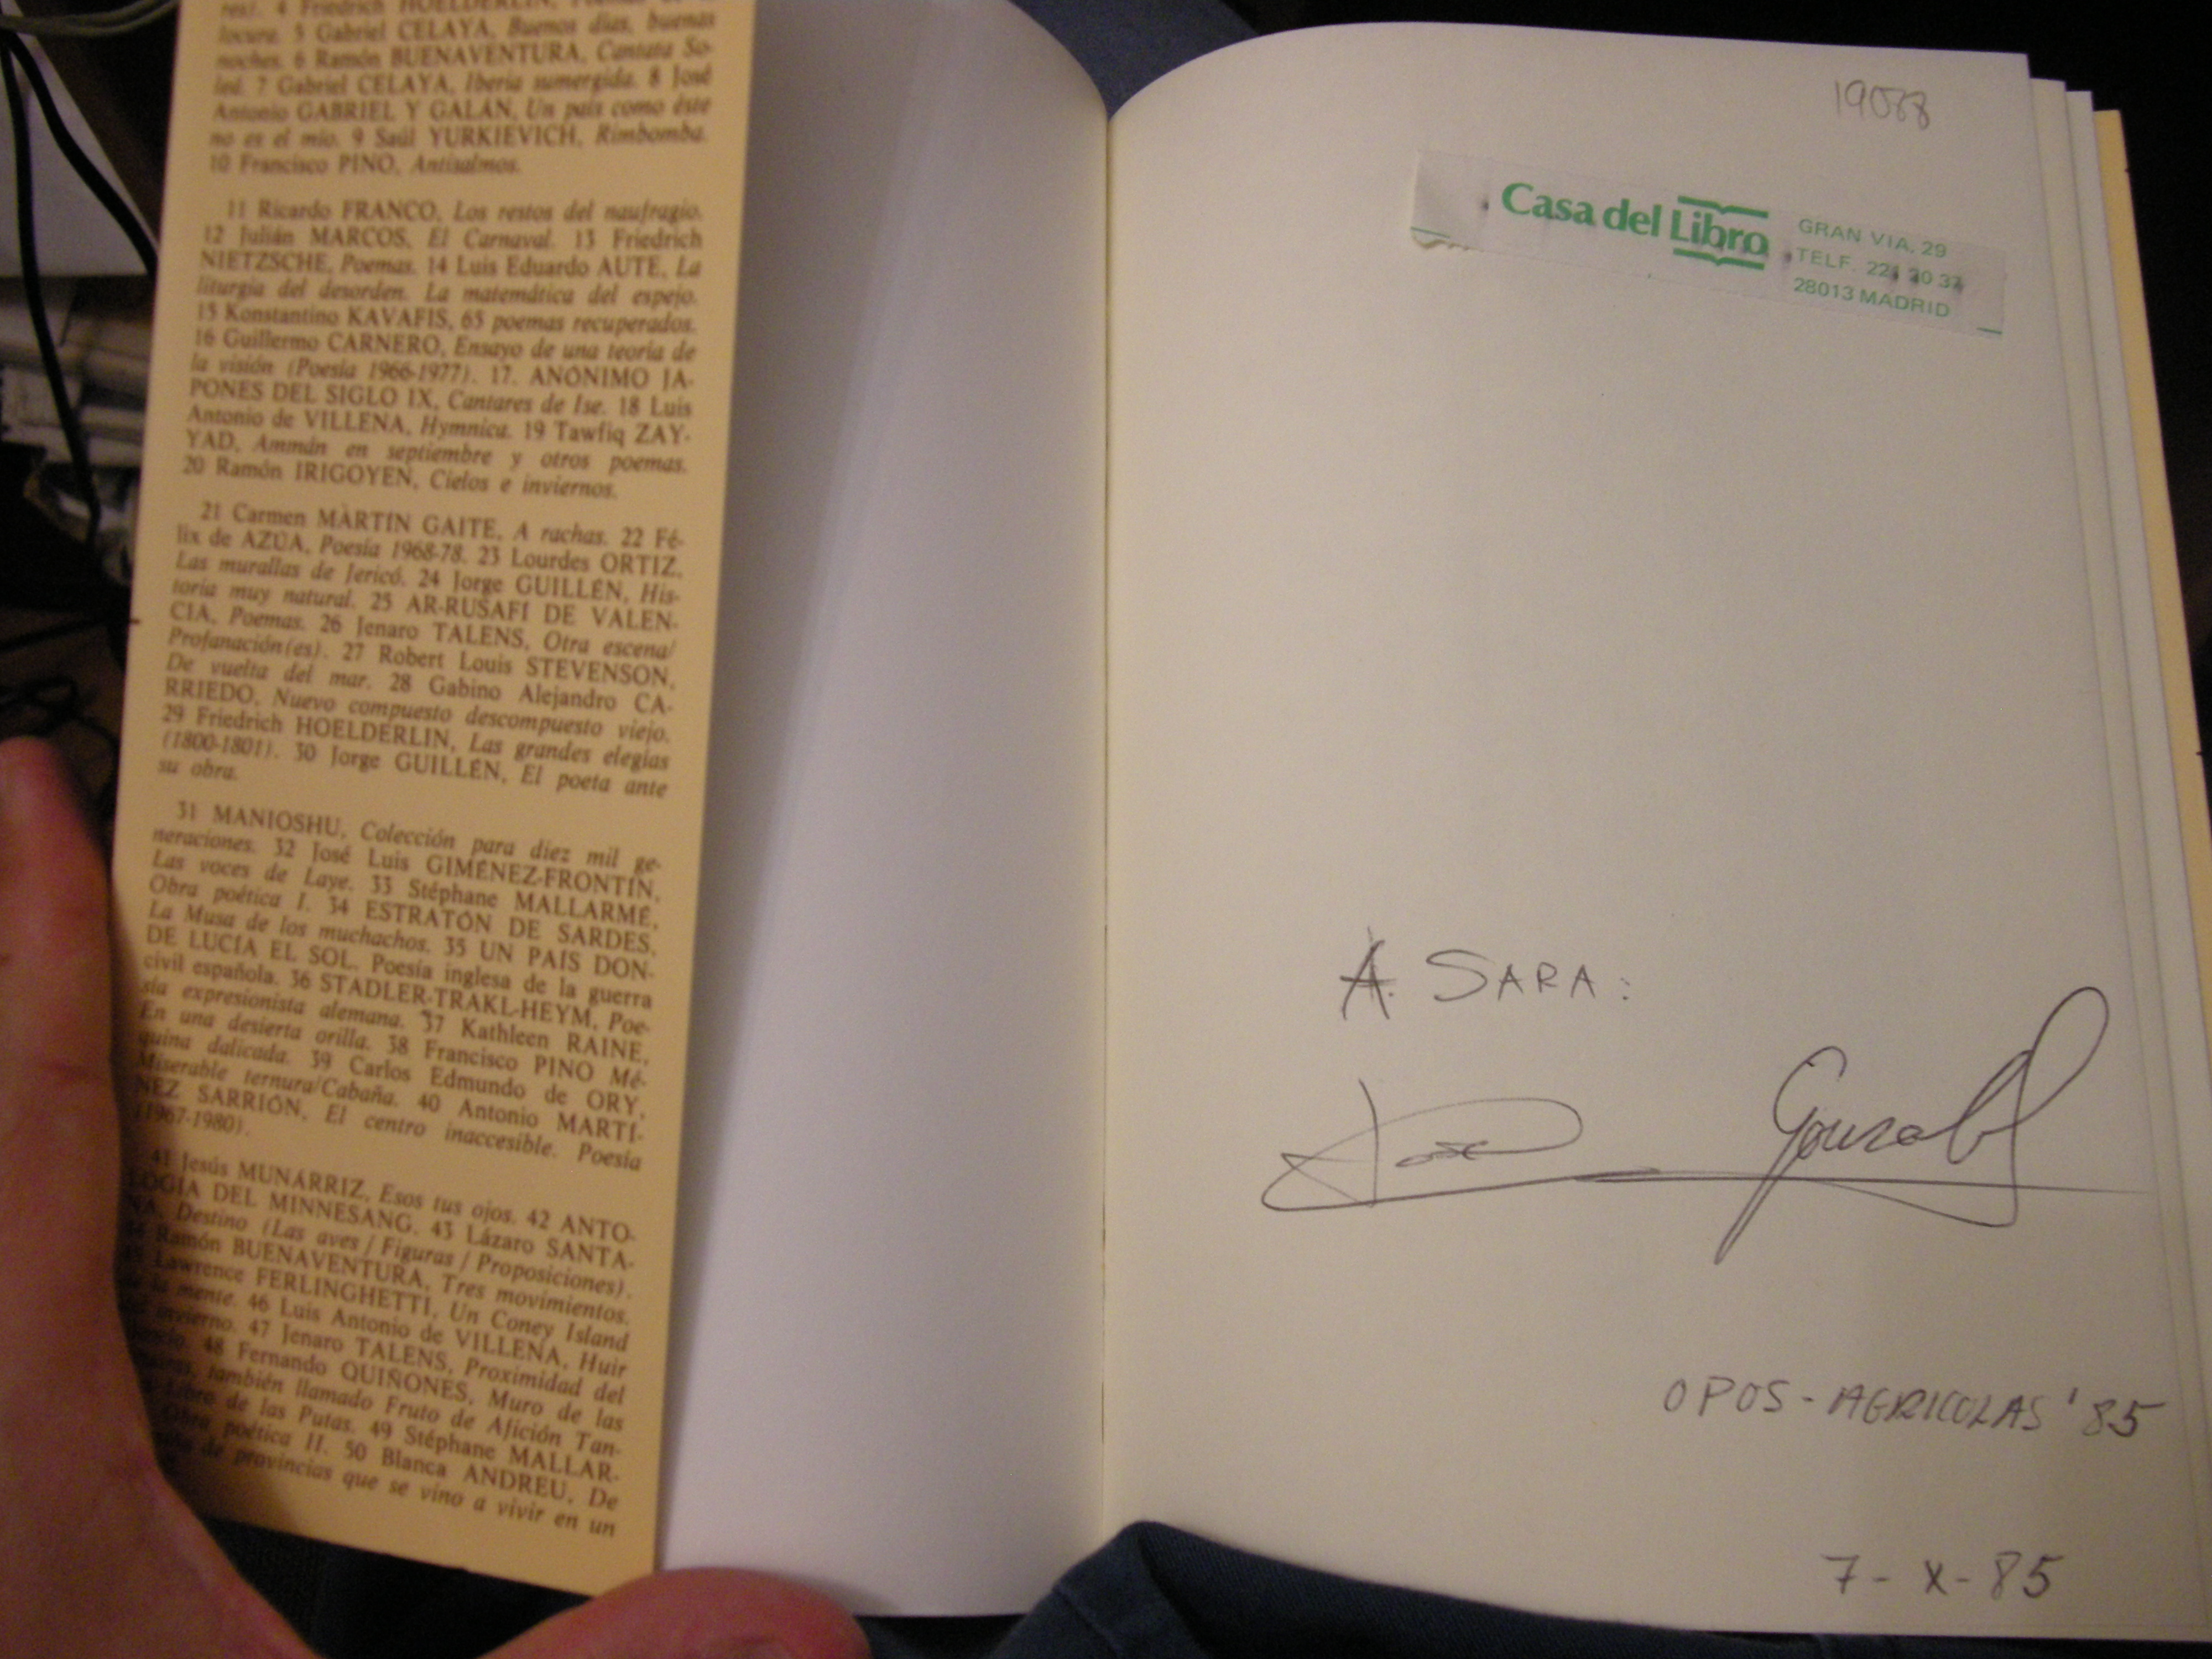
\includegraphics[width=0.75\linewidth]{images/2013/notas} 

}

\caption{*Valladolid (Spain). September, 2013*: The book F. was referring to.}\label{fig:notas}
\end{figure}

``\emph{The mirrors don't know how to lie anymore},''\footnote{\emph{Los espejos no saben mentir}} says a song by \href{https://es.wikipedia.org/wiki/Diego_Vasallo}{Diego Vasallo}. Judged by the absolutely flawless condition, better than most of newly released books and bought in bookstores, she didn't even open it. Probably, she must have moved out from her place, why not because of the crisis, to a smaller flat, maybe after a separation, and she would do away with part of her library.

Ellipsis.

Good luck in your days before the start of Europe.

\begin{figure}

{\centering 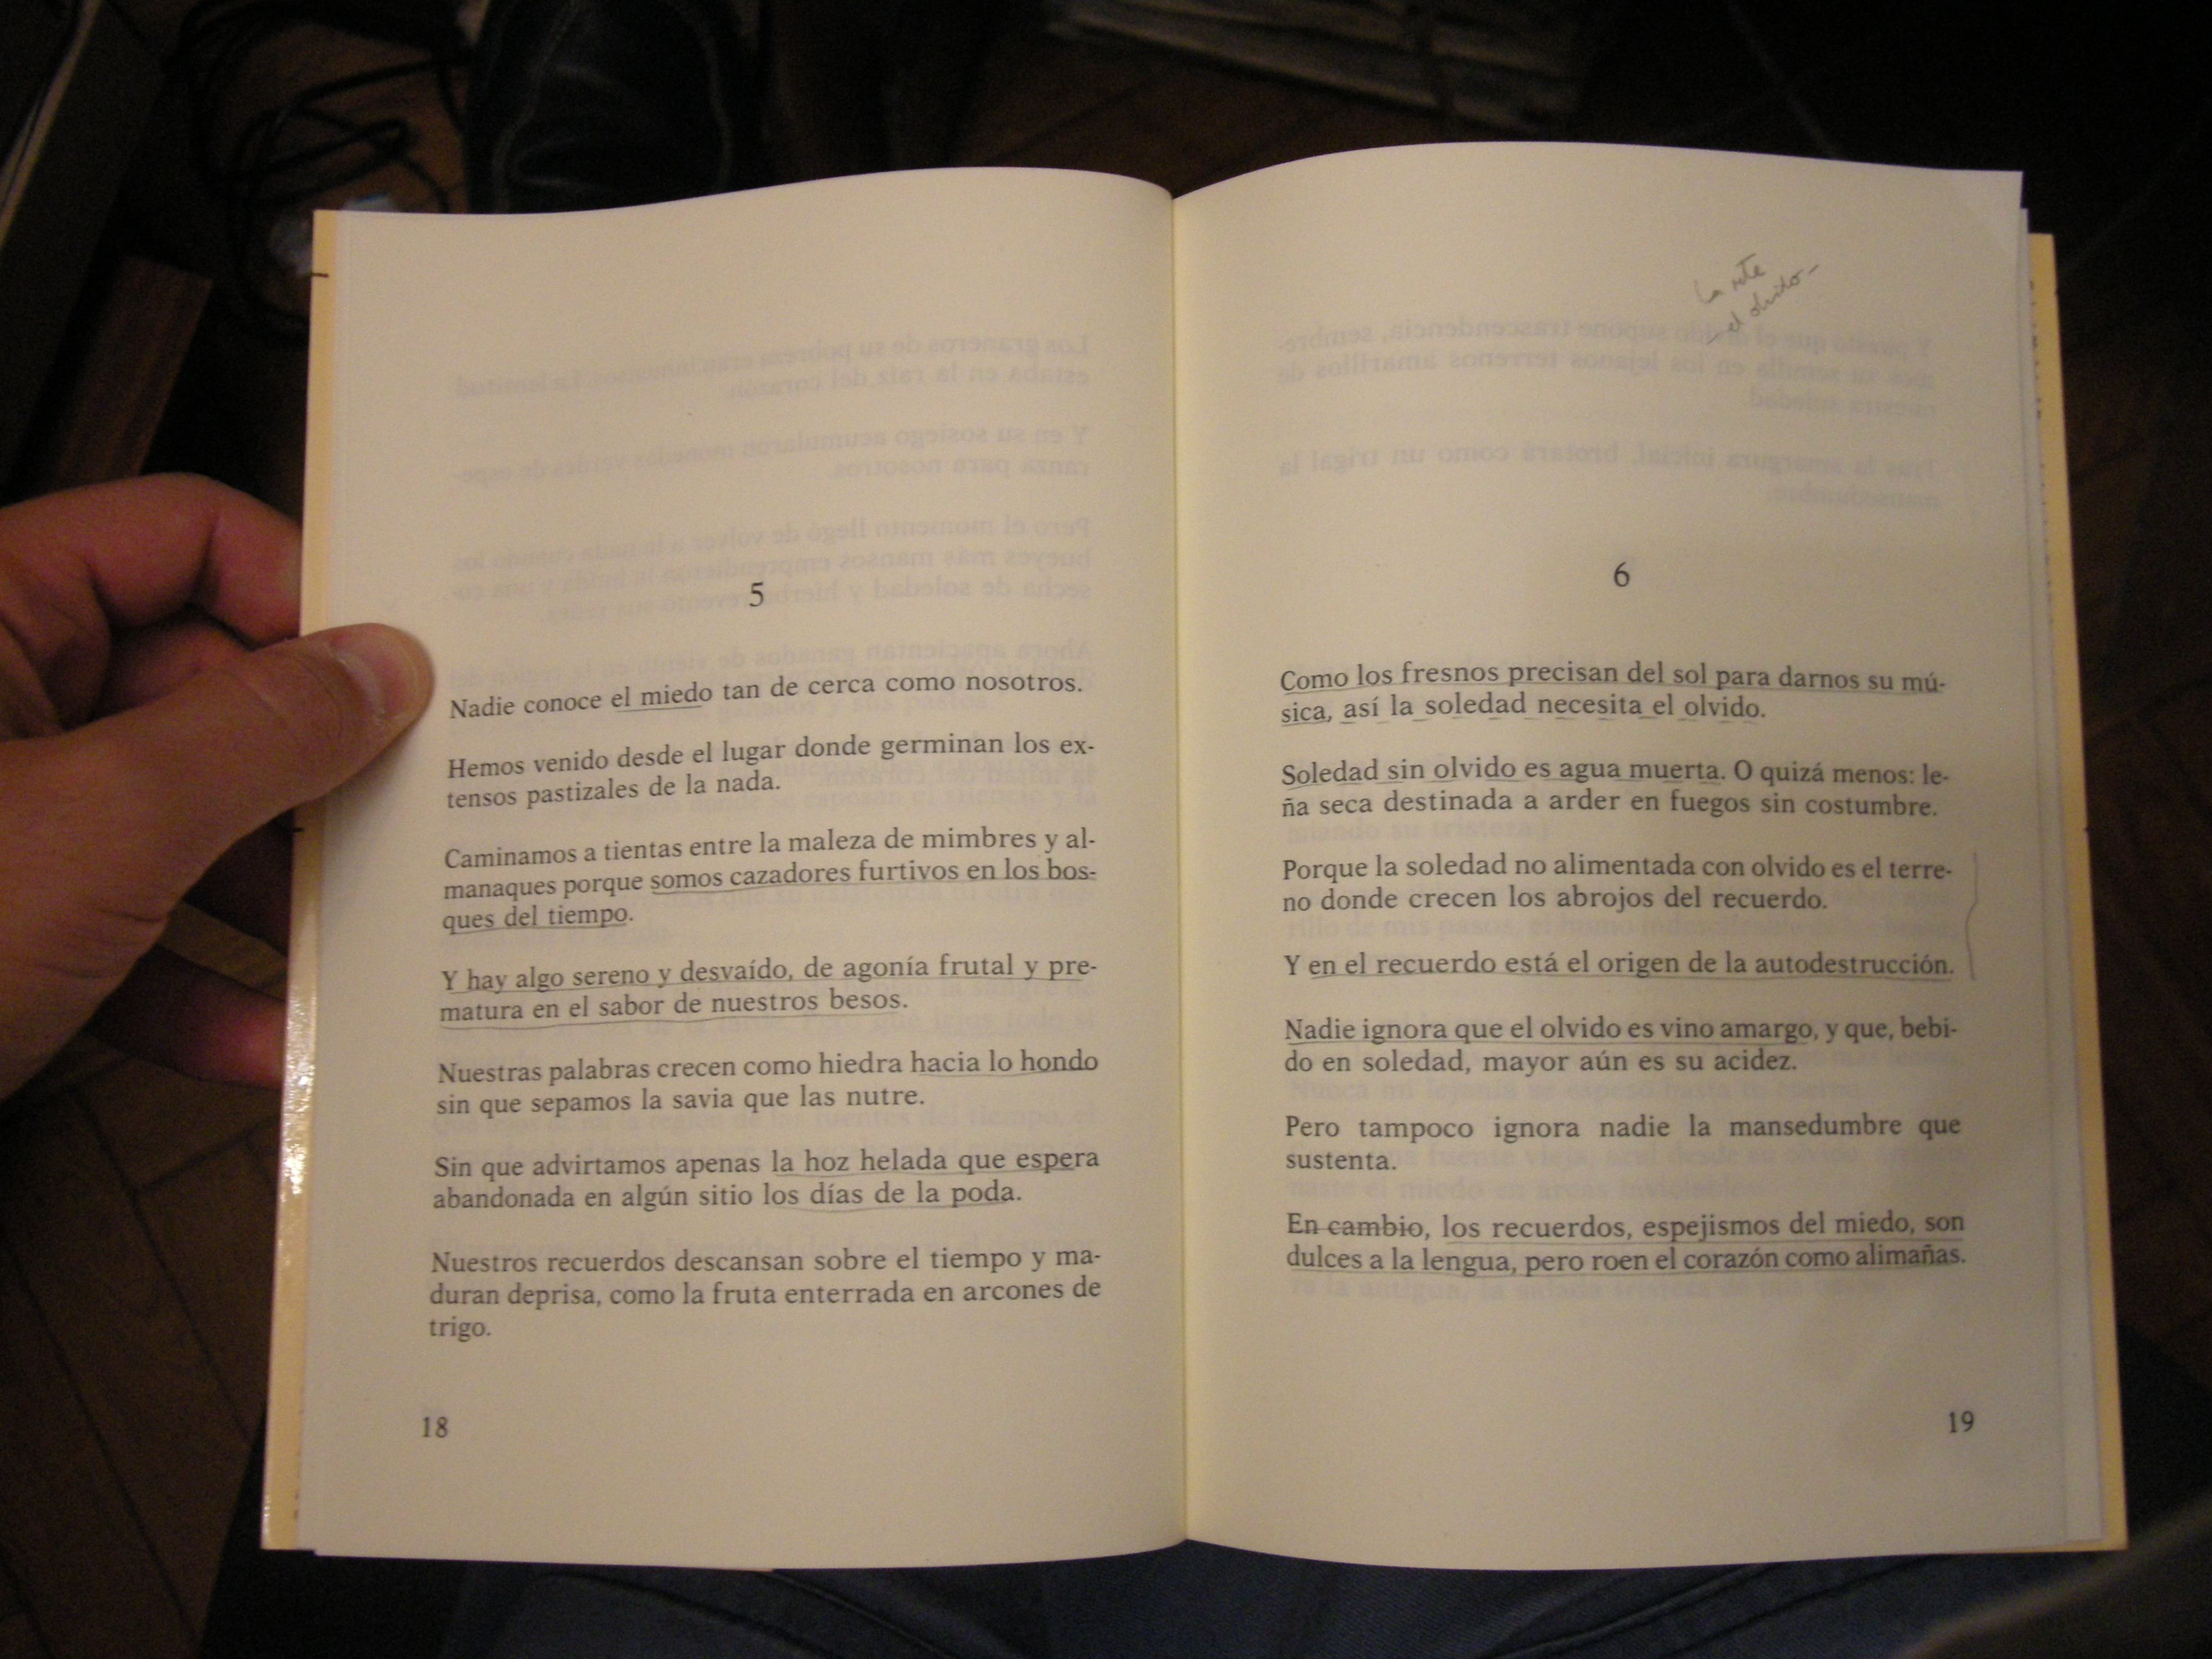
\includegraphics[width=0.75\linewidth]{images/2013/poemas} 

}

\caption{*Valladolid (Spain). September, 2013*: Some poems from the book. Sorry for the lack of translation.}\label{fig:poemas}
\end{figure}

\begin{center}\rule{0.5\linewidth}{\linethickness}\end{center}

Incredible F., the life of books\ldots{}

And how they know how to walk their own path, remember that you are not the final destination of that book, only a key piece in its progression. :-)

Who has found whom?

I am reading \href{https://en.wikipedia.org/wiki/One_Hundred_Years_of_Solitude}{\emph{100 years of solitude}}. Left half finished years ago\ldots{} Mastery. I think that the first chapter is quite anti-science, but we will have to wait for him to define his position, if that is what he will do.

Greetings and enjoy your long-awaited and deserved treasure.

I have to make blog posts and, even more than illicit, I will occasionally ask you for information from your huge artistic and literary culture.

\begin{quote}
\emph{And in the memory is the origin of self-destruction}\footnote{\emph{Y en el recuredo está el origen de la autodestrucción}}
\end{quote}

Wow\ldots{}

\begin{quote}
\emph{Instead, memories, mirages of fear, are sweet to the tongue, but gnaw the heart like vermin.}\footnote{\emph{En cambio, los recuerdos, espejismos del miedo, son dulces a la lengua, pero roen el corazón cómo alimañas.}}

\citet{llamazares1985lentitud}
\end{quote}

Pffff\ldots{} And I was thinking of imperfect past tenses\ldots{} Even worse, subjunctive\ldots{}

Carlos

PS: What is said is debt\footnote{In reference of one of our face to face meetings}. \href{https://en.wikipedia.org/wiki/Why_Beauty_Matters}{Why beauty matters}

\hypertarget{Excusas20130916}{%
\section*{\texorpdfstring{2013-09-16 Buddies program 2013\footnote{Entry of \href{https://excusasparanovolver.blogspot.com/2013/09/buddies-program-2013.html}{\emph{Excusas para no volver}}. I remember that I spend the evening with a group of internationals that spoke English in a way that I barely followed the topic of the conversation. I survided, though.}}{2013-09-16 Buddies program 2013}}\label{Excusas20130916}}
\addcontentsline{toc}{section}{2013-09-16 Buddies program 2013}

It is when you open your eyes, you weak up from the dream, from that sweet deception; and you think you've already gone to sleep. But you're still at the desk. The novelty is the temperature. Icy when still young. Glacial at sunrise So are the nights. It only congeals when the soil is dry. More forceful the fall then.

But we all like a couple of ice cubes in the drink. ``\emph{Spain is different, you know?}'' I will save easy jokes about our English. I'm not sure where they are used the most. In Europe, they are merciful, perhaps somewhat protective. Enough we have with our stuff, besides we laugh before they can do it. Originality, we are not lacking.

To the fifth, or sixth beer; when, if you have avoid them, you begin to understand what they say; inhibitions disappear. Lucidity allows to observe. Expectant spectator.

``\emph{What is he saying?}'' Yes, another joke about Spain. You looked great when you pretended to be nice to me. The important thing is to participate. Even 5-year-olds say so. We still don't believe it.

You also discover the differences. In Denmark the university is free. Things that are achieved with 60\% of the salary in taxes. Ah! 650€ of scholarship every month. For pens, rules, maybe a new iPhone.

Another round of beers. Two more and it's up to the Spanish \ldots{} He starts having rough times already. We talk like this in Spain, do we have much more to lose? Yes, pride. Because the Stella Artois at two euros each for 10 people are equivalent to half a week based on rice and pasta. We drink like Belgians, and we eat like Chinese.

``\emph{We are different. A kind of fun mix. A weird one. A stupid one.}'' Can't it be possible just sit and talk? Obviously not. Welcome to the twenty-one century. Whoever wants to learn English go and read something else. (Welcome to the twenty-first century.)

So, in those we are. Internationally representing our \href{https://www.youtube.com/watch?v=tctViHyZeJY}{great Olympics games}. \emph{Du yu nou guat ai min?}

Simply disgusting. It is what it is. You cannot make a silk purse out of a pig's ear.

Let the train take us in second class and with a Go Pass.

\hypertarget{toF20130917}{%
\section*{2013-09-17 Poem to F.}\label{toF20130917}}
\addcontentsline{toc}{section}{2013-09-17 Poem to F.}

And recount the times it hasn't happened

About how close you were left

How far you could have been

How wrong you always were

there are things that do not change

Reality dwells behind your gaze

But memories play hide and seek

When you count to one hundred

The game is over

We all run for the afternoon snack

Winning doesn't matter anymore

It is not for the time, nor for the hunger

Mom rules

You obey

They taught you how to behave

Take the crumbs off your shirt

Aren't you old enough for nonsense

They remind you every birthday

With amazement

Until it's rude

Only the poor eat bread in that way

With pleasure

Every bite is new

is life

Now you travel by train

Sometimes first class

Until the ticket collector arrives

Looking like Swedish is valid in Haiti\footnote{In Spanish \emph{Hacerse el sueco} means \emph{To play dumb}}

Where smiles are the (only) most precious asset

In India they ride on the roof of the wagon

Mom rules

You obey

You smile

You always learn something new

Where is the school

When you look out the window at the PE class

Life is going on as normally as ever

\begin{center}\rule{0.5\linewidth}{\linethickness}\end{center}

Carlos,

When you email me at three in the afternoon, something will go wrong. ``\emph{Reality dwells behind your gaze.}''

Write every day, whenever you can. ``And recount the times it hasn't happened.''

I go to sleep. Sweet Europe. You must update me on your course. When are you starting, at least. \emph{Until the ticket collector arrives}. And you get the best grades.

Health.

\begin{center}\rule{0.5\linewidth}{\linethickness}\end{center}

Y cuenta las veces que no ha ocurrido

De lo cerca que te quedaste

Lo lejos que pudiste estar

Lo equivocado que siempre estuviste

Hay cosas que no cambian

La realidad habita tras tu mirada

Pero los recuerdos juegan al escondite

Cuando cuentas hasta cien

El juego se ha acabado

Todos corremos a por la merienda

Ya no importa ganar

No es ni por la hora, ni por el hambre

Mamá manda

Tú obedece

Te enseñaron a comportarte

Quítate las migas de la camisa

No eres ya mayorcito para tonterías

Te lo recuerdan cada cumpleaños

Con asombro

Hasta que es descortés

Solo los pobres comen pan de esa manera

Con placer

Cada bocado es nuevo

es vida

Ahora viajas en tren

A veces en primera clase

Hasta que llega el revisor

Hacerse el sueco es válido en Haití

Donde las sonrisas son el (único) bien más preciado

En India viajan en el techo del vagón

Mamá manda

Tú obedece

Sonríes

Siempre aprendes algo nuevo

Donde queda el colegio

Cuando miras por la ventana la clase de educación física

Life is going on as normally as ever

\hypertarget{toF20130918}{%
\section*{2013-09-18 Poem to F.}\label{toF20130918}}
\addcontentsline{toc}{section}{2013-09-18 Poem to F.}

\textbf{Empty note}

they are like ghosts

they appear and disappear

some ride a bike

they like the company

for a while

they sleep during the day

to make night escapes

they enjoy themselves

they look for themselves

and since nothing they find

they come back with their tails upright

proud of themselves

the rest is for dogs

\begin{center}\rule{0.5\linewidth}{\linethickness}\end{center}

\textbf{Nota vacía}

son como fantasmas

aparecen y desaparecen

algunos van en bicicleta

les gusta la compañia

un rato

duermen por el día

para hacer escapadas nocturnas

they enjoy themselves

se buscan

y como no se encuentran

vuelven con el rabo erguido

proud of themselves

lo demás es para perros

\hypertarget{depths}{%
\chapter*{The depths (October - December)}\label{depths}}
\addcontentsline{toc}{chapter}{The depths (October - December)}

\begin{figure}

{\centering 
\includegraphics[width=0.75\linewidth]{images/2014/room} 

}

\caption{*Leuven (Belgium). October, 2013*: This is the very beggining of the story, the room where most of these letters were written. I started there to use a fitness ball as a chair. And that lovely [Pangaea](https://www.kuleuven.be/english/studentservices/pangaea) mug.}\label{fig:room}
\end{figure}

\hypertarget{tot20131110}{%
\section*{2013-11-10. To T.}\label{tot20131110}}
\addcontentsline{toc}{section}{2013-11-10. To T.}

\begin{figure}

{\centering 
\includegraphics[width=0.75\linewidth]{images/2014/explorer} 

}

\caption{*Leuven (Belgium), September, 2013*: The 24th. My 20th birthday. I was exploring the center of the city, enjoying the free beers that one gets only by showing your ID and proving that it is your birthday. Fleeting happiness...}\label{fig:explorer}
\end{figure}

Leuven, 11\textsuperscript{th} of October of 2013.

Greetings T.,

How is everything going? I hope that well and without too many frights.

I attach a letter explaining some of the thoughts I have had in my mind during these months.

I mentioned my intention to call you during my stay in Barcelona but, as I explain in the letter, I preferred to use writing as a means of communication.

My trip to Barcelona has left me in a rather strange state of longing, melancholy, and loss of comfort\ldots{} I do not know if these beautiful three days I have spent there have been beneficial or harmful.

Greetings and thanks,

Carlos

\begin{center}\rule{0.5\linewidth}{\linethickness}\end{center}

Leuven, 10\textsuperscript{th} of November of 2013.

Greetings T.,

I hope everything's going well. Remember that the time we have is to try to live as best we can. Knowing our limits and trying not to exceed them.

The first thing is to apologize. You're going to read something that, I suppose, will cause you discomfort and disgust. It'll probably influence you emotionally and intellectually. My ideas, let's hope, can't influence you, but I sense my mood will affect you. Empathy is within our human condition, as our compassion for our neighbor, which many of us forget and is left only in exceptionality. Like yours. I'm so sorry that you have to read this letter. I'm really sorry. But the situation is becoming more complicated at an unexpected and alarmingly speed. I feel pushed to ask you for help; to take on the role of psychologist and priest-confessor, (ironic considering how much you don't like priests\ldots).

T., please take your time to read and answer this letter. My problems are not in a hurry. I know your advice will always be of incredible quality, so it will be worth the wait. I also don't want my problems to get in the way, more than they already do, and they're going to do it, in your pace of life, in your priority issues, much more important than mine.

Regarding the communicative medium, writing, I have preferred to use this letter because of the ability to reflect and reread that allows us both. In this way, we can present our organized ideas and retrieve the exact information if necessary. I don't know if a phone conversation or a face-to-face talk would have a greater short-term impact, but the memory is very fallible. This is not, for me, a transient problem that can be solved with a coffee. It is settling into my soul, in my being, and in my mind, unconsciously and insidiously. As far as I believe, it is necessary to root it out and make future revisions so that it doesn't regrow. Still, at Christmas (Winter Festivities) we'll have a coffee and catch up.

I will use the metaphor to help express some ideas, as my intellectual resources are markedly limited. But I would appreciate advice without and abusive use of these, unlike I have done. I would like to see clearly the way to be followed and avoid possible misinterpretations. Still, the beauty of your words and the power of the images that your metaphors can create will be a great encouragement in my disoriented search for a right path.
I'd like to tell you a few things that are hanging around my head over the last few months.

Probably the source of the problem, or a factor in its appearance, was the reading of a book: \href{https://en.wikipedia.org/wiki/Pulp_(novel)}{\emph{Pulp}} by \href{https://en.wikipedia.org/wiki/Charles_Bukowski}{Charles Bukowski} \citep{bukowski2002pulp}. I did it as a language exercise, to improve my English, but its message has insidiously meddled in my thinking. Unconsciously. That hatred, that banality, the death, the impoverished quality of the human being of the twenty-first century, the disorder, the violence\ldots{}

For similar reasons, I'm no longer sure I want to read poetry anymore. The idea of death appears repeatedly and spontaneously in my thinking. It's uncontrollable. Sometimes it blocks me, sometimes it depresses me, others it causes me frustration or anger. The multiplicity of interpretations offered by poetry, and my pre-activated mind, make me detect constant references to death. I can't get rid of the idea. It's lodged in my brain.

This thought has led me to value the importance of life, a human being. But wrongly, I hope, I only see banality, hopelessness, a continuous wandering towards an inevitable destiny. The nonsense. This society is sinking at an alarming rate. It's sinking unstoppably. We're heading for the abyss. I'm losing my faith, my hope.

Besides, something dangerous and new is appearing in my way of being. I'm starting to feel hate. A deep hatred towards mediocrity. A hatred that begins to take root in my heart, in my soul. It catches me in social situations, at mass parties filled with crowds without any purpose. Anesthetizing our senses, with noise, low light, and alcohol. I admit my enormous guilt since many of these thoughts of hatred manifest more intensely if I find myself under the influence of drinks. My instincts are revealed, my hate manifests.

I have not had any physical fights, for I have never been a violent person, by ability and principles. I consider that intellectual capacity and aggression are inversely related. The higher the amount of one, the less of the other. Only when we feel frustrated and scarce in resources does aggression and physical violence appears.

Despite the absence of physical violence, my words and thoughts portray powerful hate. My intentions are, indeed, aggressive and violent. I'm not able to start a conversation that doesn't lead me to an argument or a clash. I start incriminating the other person, judging her, considering her mediocre, inferior, banal. Things get worse if I try to advise her, showing my point of view, instruct her, even. Who am I to teach? In those moments the confrontation is absolute. The other person gets tired and usually runs away. I still have hate-laden bullets ready to fire.

F. doesn't help. I think part of this mentality is generated by him, by his verses, his ideas. It's made me hopeless. Another friend of mine, C., who has a very powerful mind, has also led me down a path that I am not sure is the right one.

Both C. and F. have opened my eyes, they have taught me the world of shadows in which I was living. They have pushed me out of the cave. I'll always be indebted to them. But, I think, they're not treating people who continue inside the cavern properly, living out of shadows. They despise them, they abandon them, they repudiate them.

I want to believe that the people left in the cavern, in the banality, should be helped. But the empire of Facebook, Twitter, the Internet, and WhatsApp controls them. Their ideas are now within me. I'm afraid of this situation, it makes me nauseous and disgusted. I'm repulsed by people who are imbued, drowned. They prefer to continue to be fed with vacuous dreams, for not facing the truth.

In the direction towards the exit, I hope, halfway through, I start to see the light. It blinds me. It aches and hurts me. Sometimes I wonder if it's better to keep living in the cave, comfortably, quietly and futilely. Outside the wind intensifies, and I'm not used either to nudity, transparency, nor loneliness.

I know I'm doing something wrong. I'm misinterpreting something. Or it may be that I am fighting for a lost cause, and I should embark alone on my personal goals, (An ethical force blocks me). Or should I go back to the cavern, to the blindness and join them? (Having approached the light, the truth hampers this option). I feel weak. I need support all the time. I have powerful social needs that drag me to stay inside, living out of shadows. I'm pretty lost and disoriented. I'm thinking of going to therapy to be fooled into fooling myself. Getting into the warmth of the cavern, to see the shadows and wait for death seems to me as the most feasible option.

I'm loosing out on the experience of studying in a foreign country with all these thoughts in my head bombarding and bothering me. I can't taste the beauty of diversity. I forget the power of human warmth. A few weeks ago, we had a class on the relationship between happiness and social relationships; the sadness of loneliness, of the lonely one. My nature is social, very social. I used to be happy. I'm aimless now.

I think only a person as exceptional as you can give me some guidance and good advice. I need some information to make the lest incorrect decision as possible. To get out of the trap I've built myself.

You can't imagine, T., how lucky I am to have met you. How much I admire you and the tremendous respect I have for you. Death assaults me, all the time. Thinking about your age overwhelms me with anguish. My eyes are flooding. Thinking about the unconditionality and premeditation of our destiny is very hard. I don't know what I'm going to do when what's going to happen actually happens, with each and every one of us.

I am surprised that the oldest of my friends retains hope and believes in the future, on the change. However, youth is devastated, hopeless and lost, like me (21 years), C. (24) or F. (33).

Could we pick up the towel we threw away?

I'm sorry again for reading my problems and stealing your time.

Eternally grateful.

Carlos

\hypertarget{fromtomas20131111}{%
\section*{2013-11-11 to 13. From T.}\label{fromtomas20131111}}
\addcontentsline{toc}{section}{2013-11-11 to 13. From T.}

Carlos, good morning.

I read your letter at dawn, I have reread it afterward, and in both moments I have been worried. I had to take the dog out and clean the house, so I delayed sending you a first response. I have to write slowly, and this morning I have it a bit complicated, with some commitment that cannot be postponed. I hope to sit down this afternoon so I can send you an answer that can help you. For now, I just want you to feel that your mail has not gone to outer space and that its recipient is entangled with other things as if friends did not occupy the first step of life at the level of priorities. Leibniz, Pierre Bayle, and some other things can wait. While I sit down and order my head a little, it occurs to me to send you a couple of readings that I hope will help you to reconsider some things, especially that dark and pessimistic tone in which your letter moves. The risk of depression is always there, close to the edge of any step. It's what it takes to be human. But depression is a disease, I'm not going to be the one to analyze it to the psychologist you are and who understand it well. You know very well where and how you are, and I am very happy that you come out of yourself and that you trust your friends, in me, although I am not sure that it will be able to be that crutch that will help you to walk. I will try, although you know very well that the way you have to walk it yourself; the others will not be more than a minor walking stick in the best of the cases.

Searching in my memory for things that I have read and that can serve you, I have thought about authors like \href{https://en.wikipedia.org/wiki/Bertrand_Russell}{Bertrand Russell}, who won the Nobel Prize for Literature in 1950, and who has been one of the most important mathematicians and philosophers of the 20th century. He wrote with a wonderful English. There I send you a Spanish version and the original in English of his \href{https://russell-j.com/beginner/COH-TEXT.HTM}{\emph{Conquest of happiness}}\citep{bertrand1930conquest}, in case you want to practice English, with the literature and the thought of someone who had a very complicated life, more difficult than it seems at first sight, but that always maintained the control of himself and the pulse of life. The second reading is by \href{https://en.wikipedia.org/wiki/Erich_Fromm}{Erich Fromm}, \href{https://books.google.de/books/about/The_Revolution_of_Hope.html?id=SVdy0rtho0kC\&redir_esc=y}{\emph{The Revolution of Hope}}, whose original English I do not have and not found on the Internet, to download for free. Anyway, I hope that the Spanish copy will be useful. I hope these readings serve you, which I imagine will counterbalance Bukowski's stark realism. Writers write how they live, although some say they are transfigured. Bukowski is a clear example of how a writer manifests in his literature as he lives, and the life of this person was not exactly an interesting life or deserving of imitation, although it has contributed to literature a work that deserves to be analyzed. But not all readings are the most appropriate at any time. The same thing happens with music: there is music for every instant or, better, for every moment, situation or state of mind. I would balance a depressive mood with Mozart or Haydn, for example. In any case, depending on how you see yourself, you may have to seek help and put a lot of effort on your part to get out of depression.

Well, let's see if this afternoon I can sit with time ahead and I can answer you from the rationality and with the heart in the hand.

When I tried to attach Russell's file in English, I saw that it is very large, so I can not send it to you in this same email, which has a sending limitation of ten megabytes; therefore, I send it to you in another email.

A hug.

\begin{enumerate}
\def\labelenumi{\Alph{enumi}.}
\setcounter{enumi}{19}
\item
\end{enumerate}

\begin{center}\rule{0.5\linewidth}{\linethickness}\end{center}

\begin{figure}

{\centering 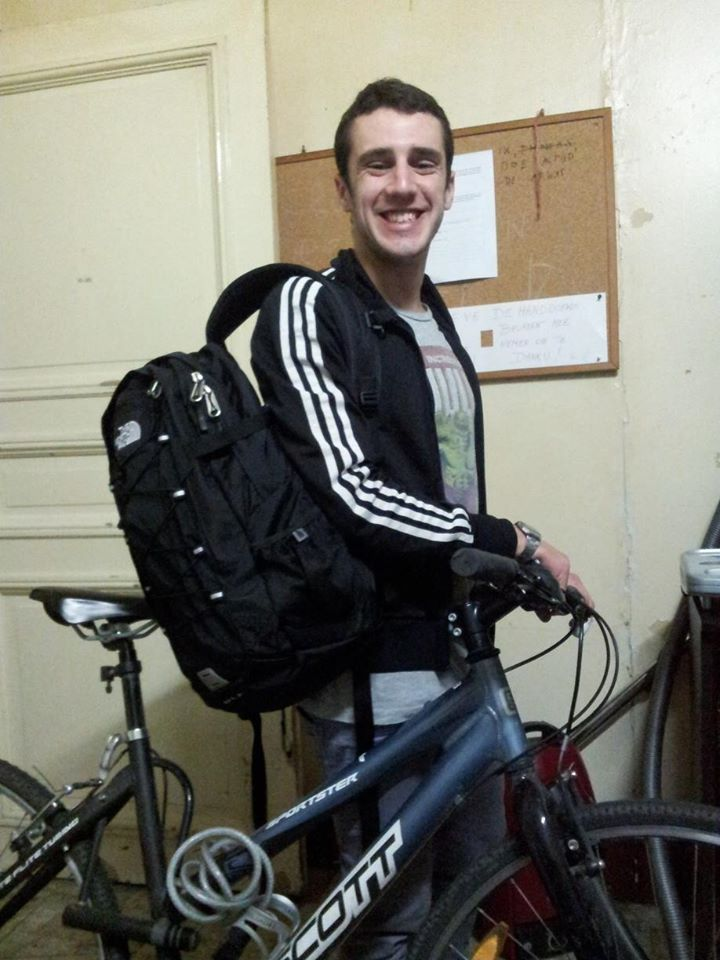
\includegraphics[width=0.75\linewidth]{images/2014/bike} 

}

\caption{*Leuven (Belgium), October, 2013*: I was happy when I settle down. I had my new NorthFace backpack and I was ready to ride around. However, things went differently... }\label{fig:bike}
\end{figure}

T.,

Thank you very much for your very quick response and your concern for me.
I go to the library to read Russell (I have an e-book, but it is for occasions when the paper is scarce). I think that is exactly what I was looking for. I hope it does not take more than a couple of days to read it. I'll tell you if it's making a mark on my character.

The road is walked alone. And you sent me a pair of good shoes to start walking. If you have priorities, accomplish them. I'll be busy with Russell and Fromm.

Health and thanks.

Carlos

\begin{center}\rule{0.5\linewidth}{\linethickness}\end{center}

Carlos, good morning. We have a sunny morning around here; I hope you can also enjoy a sunny day and, above all, I hope and wish that today you are better than three days ago when I received your letter. I send you in Word format the answer to your letter. I do not know if I have elaborate on it too much, I simply hope that my meditations can serve you, although I know that in those, as in yours, I address many questions. With that purpose, I have written it. It has taken me longer than I would have liked and what I envisioned three days ago, but I have not been able to finish it before. I hope to see you soon, to be able to drink coffee together - you know, I will take a small juice\ldots{} Oh! I should not say it, but you know that you have me at your complete disposal.

A hug.

\begin{center}\rule{0.5\linewidth}{\linethickness}\end{center}

Valladolid, 11 November 2013

Carlos, good afternoon.

I have carefully read your letter, which is very intense and sincere. It has no waste because in it you perform an exercise of sincerity, which only fits when you address the person with which you have full confidence and when the inner voice not only does not stifle but remains and even increases. This exercise of communicating our problems allows us to look into a mirror and we can analyze them and do it with ourselves with some objectivity. Moreover, this exercise, which manifests the need to face problems head-on, indicates decision and intelligence, qualities that you have always had. You can be sure that, even if you do not ask me in your letter, I will keep absolute confidentiality regarding the content of it.

It's not easy to get started, because you approach your personal circumstance in your letter in a complex way, and the answer can't be easy. Everything we do has significance and reading has a lot of it. No reading is inconsequential to the reader; there's always something that, like fine rain, soak through. The readings, moreover, do not wet the skin but are directed to our sensitivity and understanding. Surely, the psychological procedure becomes in that order and is first directed to our emotional, and not rational, the sensibility, to face our understanding later. But the traces of situations, approaches, ideas, language, and even the style that appear in books somehow permeate our sensitivity. There are books - novels, essays, poems - for all tastes and situations, but not all are suitable at any time in our lives. There is always something to which, consciously or unconsciously, we are inclined to read one thing and not another. When reading for pure pleasure and not for an academic obligation, for example, we must choose readings according to the inclinations or needs we have at each moment. All the works are interesting, but this does not force us to suffer from their reading; there must always be enjoyment in it, and something else, we must seek to read while keeping intact the ability to distance ourselves from the content of what we read. It is the only way for us to soak in reading, but for us and not the author to do it through our sensibility. In addition, it is the way for us to make the most of what we read. That estrangement, that kind of necessary \href{https://en.wikipedia.org/wiki/Epoch\%C3\%A9}{\emph{epojé}} makes us smarter (from Latin \href{https://www.allwords.com/word-intellect.html}{\emph{intus legere}}, read the content inside it, penetrate its interiority), that is, it allows us to reveal how much is structural and hidden in what we read. I know it's very easy to get involved in the content of reading, especially when we have a great story in our hands. But the story is great because it serves as a vehicle for complex and deep content; these are what's interesting about the novel or the poems. I think we suffer from a certain educational or formative deformation, derived from the way literature has been taught and the trap that involves authors moving ideas and attitudes through stories. This is an art, but the reader must know how to allocate each thing in its own place. The little I have read from Bukowski has led me to think that his style many times, though not always, brutal and grim conveys ideas of contempt and violence, a conception of reality devoid of humanity, as if reality, people and things, were there to beat them. Acknowledging that Bukowski was a victim of himself, I can understand that the content of his works is the living or clear expression of his own personal situation. This doesn't mean he shouldn't be read. I myself have approached at some point his poetry and, although it is not the style and content that I like the most, it can be read, as long as it is done as I was saying, with distance, with a good mind awake so as not to fall into the claws of so many affirmations -- denial is a form or modality of affirmation- as conclusive and the repetition of ideas such as that of death or others such as prostitution or the reification of human life. \href{https://en.wikipedia.org/wiki/Jaime_Gil_de_Biedma}{Gil de Biedma}, like other poets and writers, wrote almost always under the influence of alcohol and it is perceived in his poetry that in his pen there is something that moves it and that is beyond soberness.

Books that are read must behave like friends. I know that a book lacks a life of its own, that it does not have a heart or a sensibility that speaks directly to us, but that it is the readers who perceive its heart and its sensitivity, which is not always the same for all. It is not the book that looks us in the eye or caresses us, it is us who project on it and from it its content on ourselves; it is us who feel and interpret its content, often far removed from the intentions of the author himself. Hence I infer that books and authors, like individuals, should be the subject of choice on the part of the reader, who has in his hand the final decision. I don't think \href{https://en.wikipedia.org/wiki/Franz_Kafka}{Kafka} is an author to read in times of psychological weakness; however, he is a fundamental writer, who must be read under the appropriate psychological conditions of the reader and, as I said in the previous paragraph, with the necessary distance to fit into the soul of his work. A work like \href{https://en.wikipedia.org/wiki/Georg_Wilhelm_Friedrich_Hegel}{Hegel's} \href{https://en.wikipedia.org/wiki/The_Phenomenology_of_Spirit}{\emph{The Phenomenology of Spirit}} \citep{hegel1998phenomenology} cannot be read without a solid formation on philosophy because that work will behave upon the reader as an enemy if we lack it; it will be like an immensely tall and abrupt mountain range, impossible to encompass. Books and authors have their time, so their choice is critical. It is difficult to know in advance whether what we have chosen is the right thing, if it will bring us something positive, like friends, but we will know it right away, the moment we come into contact with the work. Therefore, with books we have to act like with people, we must discriminate them according to the friendliness they awaken in us. If Bukowski is not a good company at a time, his reading is discarded, and absolutely nothing happens. There are moments to read \href{https://en.wikipedia.org/wiki/Ovid}{Ovid's} \href{https://en.wikipedia.org/wiki/Tristia}{\emph{Tristia ex Ponto}} \citep{wheeler1924ovid} and others to read the Epigrams of Marco Valero Marcial. Reading should serve to lift our spirits, not to be angry, oppressed, or depressed.

Depression is a terrible disease. I'm not going to show you anything, but it's you who could speak out broadly and with a sense of this disease. But it is a disease that places us on the edge of nothingness, nullifies us and enslaves us in the dark, preventing us from being ourselves, even though, when we go through depression, we think that we are authentically ourselves. It is us in our full selfhood when we are in full mastery of ourselves, when our qualities or abilities (I do not like the term competences) shine, are in full force, and during a depression, these are darkened, as covered by a great veil that suffocates them. It is a state from which one does not always come out by oneself, but with help, although one does not come out of it without putting effort, tenacity, and willpower. I don't know how you feel; nobody knows it better than you and no one better than you to determine if you need help or if you have enough strength to get out of that state on your own. The permanent idea of death is worrying. I confess that I have written many poems about death, but it does not affect me to write about it or read verses or texts that speak of it. It is there and appears when nature wants, but I am very clear that speaking in human terms, death is the failure of life, especially when it does not arrive naturally.

On Friday, they pay tribute to my lifelong friend, to a person with whom I have lived around the clock from the age of twelve to twenty-five and with whom I have shared even money. I have enjoyed his successes and have often been a shoulder to cry on for him - and he for me, of course. He died of a fulminant cancer last July 25. He was Professor of Public International Law and International Relations at the University of Zaragoza. Above all, he was my friend and a person committed to democracy and human rights since his (our) youth. Society has lost a great mind and above all a great person. I have mourned him more than anyone in this life and I do not forgive the nature who has taken him, but I have to accept his definitive absence. As you can understand, I'll be in that homage, and I've had to accept reality. I only understand death as a moment of life, produced by nature itself. The rest, as the Stoics tell about death, has always seemed to me to be a failure not only of life itself but of the person. Adverse situations should be dealt with effort and help, if necessary. That's what friends and, if they're required, professionals are for. The loss of a loved one stirs our guts and makes us rethink the meaning of life. It does not occur to me that reading something, however intense, will affect us so much that we enter a personal crisis. It can make us think again, meditate so that we can specify our conception of life or things, but one must always be above what is read. Autonomy and self-control are fundamental conditions of freedom. You know that the highest suicide rate is that of the Nordic countries, geographical areas where the climate is very adverse, with hardly any solar radiation. You may also be falling victim, not only of the environment and readings but of Belgium's own climate, which has very little to do with Valladolid's, at least in terms of solar radiation.

Alcohol and drugs alienate us, deprive us of our own abilities, weakening our autonomy and self-control. I do not understand the environments of binge drinking, which are environments created and supported by interests foreign to the people. No one frees himself from problems by alienating himself, but on the contrary, he enslaves oneself to something as alien as an addictive substance that ends up being our owner. There are too many economic and ideological interests behind the culture of drugs and, in particular, alcohol and, why not, rock culture and its derivatives, which are associated with it, but this is not the time to analyze this, an analysis, which, as it cannot be otherwise, the rockers do not share. I confess that I have never been able to drink more than two wines, that I have never come close to drunkenness, precisely because, like everyone else, I have seen drunk people since I was a child and I have always rejected that state. The first drunk I met was a gentleman who got into our class, at school, when I was a kid when I was five or six. The teacher, a great teacher, by the way, treated him gently and got him out; but that show shocked me so much that I have never been able to understand or comprehend the culture of alcohol or drugs. I think I understood what that meant. Moreover, university students and young people, in general, do not conceive of the week without alcohol only indicates the lack of personal maturity of those who practice it. We do not need to be high to socialize, but rather authentic human relationships are born and grown from authenticity, whose foundations are in sincerity, loyalty, commitment and, among other things, self-control and autonomy. The rest, the nonsense that Tierno Galván could say in his day and others now about fun and its relationship with alcohol, only lead to the self-destruction and destruction of society. I will seem radical to you, but the social, cultural, political, personal\ldots{} consequences of drug culture are devastating in all aspects, and alcohol is a hugely potent and destructive drug.

Poetry is but a literary genre, although some discuss it. Whether you look at it, it is offered and used as an instrument of expression that can reach artistic heights. It is not only form and beauty, as some - to some extent F. - argue. When we use the word, we express content, with greater or lesser fortune and, if there is no content, there is no literature, there is nothing that can be valuable. Any poem impacts our sensitivity even before our understanding. Besides, we usually stop reading that poem whose reading doesn't move us. Poetry is, therefore, a very powerful weapon, like everything that directs towards our sensitivity, like advertising, for example. Next to and below the emotion and the feeling of beauty that provokes any poem translates ideas, those that impact us and, as I said before regarding readings, must be sifted by our own reflection. In any case, poetry should be read like any other literary genre, with a certain distance from the read content. This does not mean that we read impassively, but strategically that procedural estrangement allows us to understand, to know better, to feel more intensely when we read, but with the difference that we keep intact our ability to analysis, our autonomy over the other. And I think this very thing has to be done in ordinary life. We're not going to a class to get emotional, but to focus our attention on the content of the teacher's speech. The act of focusing attention means nothing more than to concentrate our capabilities - in its entirety - to be able to understand how much we hear and, to do so, we constantly discriminate against the content and distinguish the fundamentals of the incidental and capture the relationships between the different content that we consider as valuable. If we were emotionally involved in the content of the teacher's speech, we would very hardly understand the content of it and surely never get to pass the subject and finish the studies. The poet Bukowski, like F. or any other poet, must be read to enjoy and never to suffer. The Bukowski of \href{https://genius.com/Charles-bukowski-hug-the-dark-annotated}{\emph{Hug the Darkness}}, of \href{https://medium.com/poem-of-the-day/charles-bukowski-bluebird-f4e80e5000ef}{\emph{Bluebird}}, or of \href{https://www.poeticous.com/charles-bukowski/true}{\emph{True}}, for example, must be read from a distance. In any case, if a poem or a poet does not excite us and that emotion is not accompanied by positive contributions - ethical, aesthetic, ideological, etc. -- its reading is cut off and we pass on to something else. Maybe at another moment, we'll find out in it what we don't see now. But if this is not the moment, we must not insist. With reading we have to enjoy, never suffer or endure. There are poets whose readings always seem new. The classics, the immortals. To give some examples of Spanish literature: Lorca, Machado, Miguel Hernández, Gamoneda, Gonzalo Rojas or Juan Gelman. Even though they are classic, our spirit - if it is worth the word - not always tastes its texts. They are there, they are offered to us and we are the ones who choose and taste them. They are a delicacy, but it is the diner who enjoys them.

It is very typical of confusing personal moments and times of social crisis when one is tempted to see on the horizon and on his back a destiny that leads us to an irremediable horizon and end. Those of us who were born in the middle of dictatorship and saw the dictator live and rule so calmly, who perceived that Spanish society was suppressed and, worse, was submissive to the dictator's own empire were tempted to think that our own destiny was written, that there was no other opportunity than surviving as it were, because we could do nothing to straighten that twisted tusk of the dictatorship and the fate of Spain and, with it, ours and that of each of us. However, many were involved in the struggle for democracy, such as my friend A., whom I have quoted you before. Passivity leaves all possible means in the hands of the power and we are left with the citizens who are defenseless and subdued. It is true that in our society mediocrity abounds even in the positions of greatest responsibility, but this is what we have so far. The horizon is clear, and mediocrity, indifference, inaction, and even violence are gradually overcome, unfortunately never completely, but our obligation as individuals and citizens is to give our best. It is the sowing that we can and must do, it is the power that we hold in our hands and it is also our own responsibility. Turning a blind eye and taking refuge in supposedly saving selfishness leads to inaction and immobility. By this path, there would never have been a \href{https://en.wikipedia.org/wiki/Thales_of_Miletus}{Thales of Miletus} or a \href{https://en.wikipedia.org/wiki/Santiago_Ram\%C3\%B3n_y_Cajal}{Ramon y Cajal}, a \href{https://en.wikipedia.org/wiki/Evolution}{Darwinist theory of evolution} or the knowledge about the \href{https://en.wikipedia.org/wiki/Genetic_code}{genetic code}. There is the example of inaction in the field of knowledge that occurred during the Middle Ages. Involving oneself implies commitment and generosity, but without them, together with other values, such as the impulse for the search for truth, the love of justice, the respect or the dialogue, for example, nothing improves, neither society, nor companies, nor States, nor human beings.

Mass parties and great mass events anesthetize; the media anesthetize with their TV shows about frivolities; the monopoly of football, so many vacuous contests, so much banal literature, etc., etc. It's easy to complain and stay in the lament, selling the image of lament as if something was built with it. We must analyze, but the analysis, which never implies complaint or regret alone, should lead to action: to educate ourselves as best and as much as possible, to work, to research, to publish, in a nutshell, to offer society the best of ourselves; it is the way to find ourselves and create spaces of personal fulfillment that bring us happiness. We may feel rejection or aversion to injustice or lack of freedoms, for example. The rejection of something implies a choice, positioning in the face of reality and taking a stance before it, which is already an active attitude. Hate destroys coexistence, paralyzes us and places us in the anteroom of violence, with which only destroys and never builds something worthwhile.

There's one aspect that has really worried me not only in your letter but in my own life. I mean the role of the intellectual and, before all, that of the citizen. Although to some extent I have already answered, I would like to add a brief reflection on this particular issue. The problem is whether the intellectual can and should even settle for doing his work in a professional manner or whether to demand from both the intellectual and any citizen something else, a greater commitment to society. The image of Plato's cavern you quote in your letter is very clairvoyant. The wisest is not the one who leaves the cavern, since he always comes out with the help of other people, the pedagogue, in the case of platonic myth; the wisest, the one who, in \href{https://en.wikipedia.org/wiki/Aristotle}{Aristotle's} words, leads a\href{https://en.wikipedia.org/wiki/Nicomachean_Ethics}{\emph{virtuous life}}, is the one who, in addition to leaving the cavern and walking the way to the contemplation of the sun, the truth, that is, performs the ascending dialectical process, returns to the cavern in order to help other prisoners out of it -descending dialectics-. There \href{https://en.wikipedia.org/wiki/Plato}{Plato} -- and the common sense -- tells us clearly what the role of the intellectual, the philosopher, and, by extension, the true citizen is. The posture of those who believe that they have left the cavern and stand there, still, satisfied outside of the cavern forgetting its origins, enjoying and reserving for themselves the sweetness of knowledge and art, only deserves reproaches. They are a clear manifestation of the social and personal selfishness that has always occurred and that populates our time. They are antisocial beings because they only want for themselves what belongs to everyone, regardless of their social origin. Here is the foundation of the validity of universal education, of public education, which guarantees access to training to all without distinction. Returning to the cavern is an act of responsibility, a due act, forced from the point of view of moral conscience. Staying out means living in overt irresponsibility. If I am honest with you, here is the rational and moral unifying thread that directed me to teach, instead of focusing on engineering, as my teachers wanted. Do not take me as a hero, because I am not, I do not intend to present myself as an example of anything; after all, I've done what I wanted and I liked, nonetheless, having to overcome very difficult obstacles, but I haven't been the only one in this either. Doing what you like and want contributes to your happiness and thus benefits and enriches society. In short, we would all like to do in life what we like, and I think we should aspire to achieve it. Returning to Plato and those who do not have solidarity and social commitment in their minds, it can be said that they renounce a part or aspect of life that contributes to their own happiness and deprive society of a good that belongs to it.

\begin{figure}

{\centering 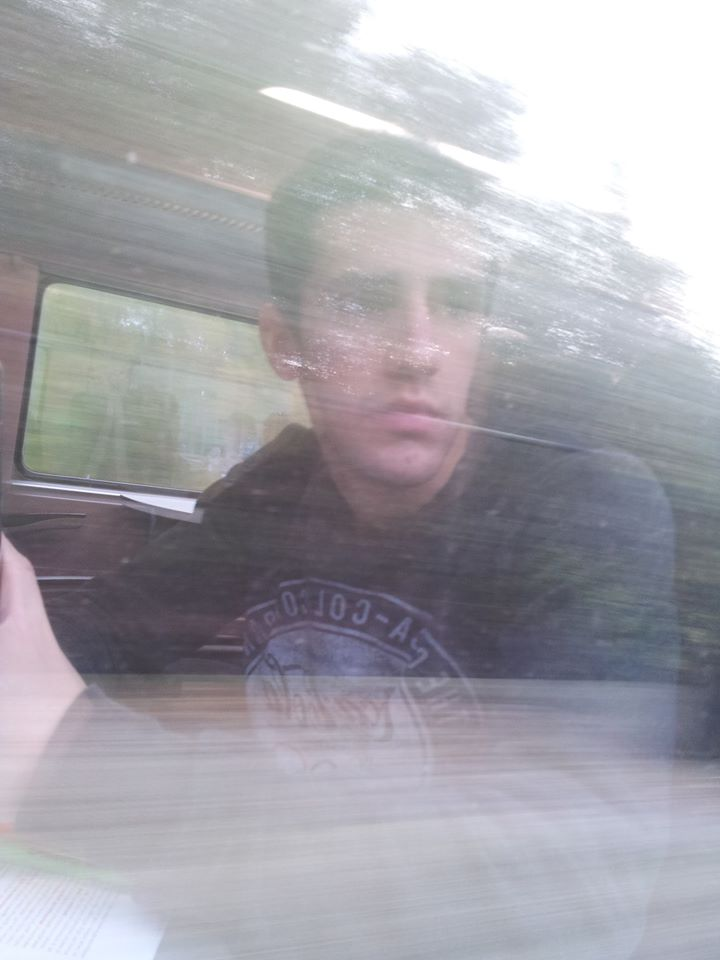
\includegraphics[width=0.75\linewidth]{images/2014/train} 

}

\caption{*Somewhere in Belgium. October, 2013*: Narcisus drowning in the train window.}\label{fig:train}
\end{figure}

Following the course of your letter, you end up with a self-incrimination meditation. I don't know if you have to accuse yourself of things. It is one thing to analyze, to stop in the way, to look in the mirror and to draw conclusions that lead to decisions that seem appropriate, another to blame for defects or faults and, worse, that this prosecution process paralyzes us and leads us to a sick situation or even sickness. The first thing must be done from time to time, as any aircraft or boat pilot does, which corrects the course at short intervals, after having done the necessary checks and calculations; self-incrimination is something else, especially when it is easy that certain circumstances outside oneself have been determinants of the personal situation: friends who do not help, personal loneliness, remoteness of family and loved ones, the weather, new companions, language, et cetera. As it happens to all of us, you may be doing something wrong, but this is no reason to fall into a depression, let alone for self-destructive thoughts or feelings to appear. You're finishing the degree you chose in your day because it was the one you liked, you've done your studies brilliantly, you have a supportive family and loyal friends to trust. You have the circumstances in your favor. I think you have a favorable career and personal circumstances for you to finish your studies in Belgium as you have done so far, taking advantage of the opportunity to study abroad, which is still a real opportunity to acquire a more open academic and personal education with broad horizons. It is you who know better than anyone the trap you have built or fallen into. Surely it consists in the aim of encompassing too many areas, widening the circle of interests and obligations beyond the degree you are studying. It is good - and necessary - that you focus on the contents of the degree you are finishing. Psychology is an area of complex knowledge with a future, which deserves full dedication. The fact that you relate and befriend people who quite surpass you in age may have led you to try to live up to their dedication to other areas of knowledge. We would all like to know everything and, moreover, to the maximum degree, but this is not possible. To grow as a person and be a good professional, we have to narrow the area of interests and especially the area to which we are dedicated. As if we were proceeding in circles, the greatest dedication must be in what we have chosen as the scope of priority knowledge; from there, other concentric circles that refer to areas of knowledge compatible with the first and complementary to each other; but key dedication must focus on the priority. The trajectory or the fruits of others' activity should not be magnified. We tend to think that what those close to us, who are moving away from our area of dedication, do is so interesting that we see ourselves in the need to emulate them. Maybe that's where we set ourselves a trap. What others do, painters, musicians, poets or scientists, whatever the branch of science, may be wonderful, but we must understand that this area of knowledge is what they chose in their day and that, precisely because they made it their priority dedication, they excel in it and make contributions to society. But how many of them do not look at others with eyes of admiration; if they were sincere, they would all reveal to us how much they admire people with dedications to an area of knowledge far removed from their own. The limitation of our time and capabilities, coupled with the increasing complexity of knowledge, means that we have to be realistic and delimit the area of knowledge in which we want to be competent and, if possible, with the maximum degree of excellence. It is from there that we gradually build the elements necessary to be happy and contribute as much as possible to the well-being of society. The rest, that we age, for example, is part of the inevitable vital process, and in which we should not think, because it is useless or worthless.

There is a thought that I have had clear since I was a child, that the future is built by us. Time, following \href{https://en.wikipedia.org/wiki/Immanuel_Kant}{Kant}, does not exist outside of ourselves, but rather is a universally necessary condition that we impose on people, the subject, on things. In this sense, although we find it strange, we own our time, which makes us owners and responsible for our lives. We are what we leave and that heritage that we leave we build it little by little, from the moment we have personal autonomy until our body ceases to have a chance of survival. Knowledge and affections, how much we build throughout life mean that sowing that we leave there as a constituent part of our own being; it is what we leave, spread among others, and that identifies us or allows us to remain beyond the limitation of the duration of our lives. This permanence does not have to always be publicly recognized, that is, by society as a whole; we stay, we remain in feelings and therefore in the memory of the nearest and sometimes even our identity is recognized beyond that limit. It doesn't matter the apparent extent of our heritage. There we left as much as we could or was in our power to leave as an inheritance. This improves life and society.

The tensions to which we subject ourselves, increased by the pressures and uncertainty created by society in general and the unique moment in which we live -- which, on the other hand, will always be unique -- place us in scenarios that are not always easy and, often difficult. Although it may seem like a utopia, good therapy is to try not to enter into the competitive game or trap that the propaganda sets us. More than just being competitive, we must be as competent as possible in that area of knowledge where we have specialized; competitiveness, that is, the place we occupy in society must be the result of our own competence, the degree of knowledge that we have reached and of what we are able to offer ourselves and others. Entering the game of competitiveness as a goal and strategy leads to stress, anguish and, ultimately, depression and, with all, to be less ourselves and even to be set apart. A conception of life as a struggle or war may seem very beautiful, as Heráclito and all economic liberalism said, but this conception is only useful to those who hold power and \emph{have} it, that is, it is -- or believes it is - safe from the swings of the all-out war of competitiveness. When those in power fall, they ask for help and demand the solidarity of others. It is a war that lowers us to the level of the animal that we are, of the mammal we are, that has to mark the territory and fight to conquer and maintain it. This new conception of reality -- which, on the other hand, is not so new and which is, for example, in the Gospel -- must be elaborated and worked, not fight, but worked to sow and flourish. A life focused on personal fulfillment, complementarity, sociability, empathy, respect, sense of duty, etc., that leads people to achieve the highest possible degree of happiness.

I think I've elaborated on a lot and I'm not sure I've written anything that you may find valuable or, at the very least, useful. I, therefore, offer you my reflections made in the thread of some of your reflections, which have seemed to me significant, among those you address or suggest in your letter. I know I've been on my toes about the problems you're raising, but I don't know if this is the right time to take each of them one by one and extend myself thoroughly. I am satisfied if my meditations help you return to yourself and, now, calmly, slowly and looking for objectivity, you will reorient your state or situation.

A hug.

T..

(Valladolid, 13 November 2013)

\hypertarget{totomas20131114}{%
\section*{2013-11-14. To T.}\label{totomas20131114}}
\addcontentsline{toc}{section}{2013-11-14. To T.}

Thank you very much T.,

I attach my answer. It provokes a very hopeful sensation the fact of communicating by letter more than by e-mail in the 21st century.

Greetings.

\begin{center}\rule{0.5\linewidth}{\linethickness}\end{center}

Leuven, 14th of November of 2013

Greetings T.,

Thank you very much for your very complete response. I have been extremely satisfied with its reading and I will read it again as soon as I have time. Your sincere and felt writing is also appreciable. I value filled with gratitude the exercise of empathy and esteem you have performed.

T., my letter is not as worked as your answer, because I write it almost in one go and without too much revision. The last paragraphs of your letter deserve a mandatory rereading, and subsequent reflection and answer. Just to mention, although I probably haven't fully understood them, I've been moved. Emotion always ahead.

Your tips are affecting me in a pretty fast and powerful way. It may be that being able to express myself, organize my thinking and look for and find a reason for my situation, are helping me to modify it. The sensation of feeling understood and heard that you transmit to me is undoubtedly a powerful effect on my mood.

I think the music I've been listening to, almost uninterruptedly, since I read your first message (Mozart's symphonies), is playing a pretty crucial role. His music is elegant and subtle, jovial and full of life. It penetrates more gently and respectfully within me than Bukowski's literature did, and its impact is, for the moment, quite powerful. I'm letting myself get soaked. I avoid the Requiem and Lacrimosa. There are moments and moments. Even without any technical knowledge in music, I can notice the impact of grim songs on my emotional state.

Concerning getting soaked, fine rains and solar radiation. I have long compared the temperature in Leuven and Valladolid. They seem to be weather-connected, as it is surprising the climatic similarity between these two cities. My source of information is the weather predictor, so I can't trust too much either. Here, I suppose, it rains a lot more. Therefore, the sky is usually greyer. But

\begin{quote}
\emph{after it rains}

\emph{like after crying}

\emph{faces}

\emph{like the sunny skies}

\emph{unwrap}

Del Val, F. \emph{Ice Tongues} \citep{val2012hielo}
\end{quote}

(There are moments and moments, poems and poems)

And if it rains intensely the sky usually gives us a bright afternoon, (when there was afternoon, now the sun dies at 18.00).

I quote the previous poem, also concerning your reflection on poetry, conscious understanding and the affectation of this on emotion. I don't think I've come to understand all the symbology or the full meaning of F.'s poem, but of all the ones I've read, this is one of those who stuck to my memory. He likes to appear from time to time, in situations where, after suffering, I see more clearly both present and past facts. I may be starting to see the light after this period of continuous fine rain, with heavy intermittent showers.

I've started reading Russell. It was a brilliant recommendation. I read it as long as time permits. I'm in the second chapter and it's amazing how well his arguments fit into my concerns. It seems that he would have written it tailor-made for me, for the contemporary man. Knowing you're not the only one helps, too.

I know the relationship you had with your friend. I don't think I'm going to imagine the suffering you've had to go through, the one you're going through right now, and the one you're going to go through in the future. These kinds of ideas and thoughts go deep, but in moments of emotional weakness they attack us and try to sink us. As the older person that you are, and given the different situations in which you have lived, you know death better than I do: its presence in various contexts, or in people you appreciated to a different extent. The little I can know about death has been taught to me by poetry, mainly that of F., as in the poem \emph{the slowness and the absolute}, or in:

\begin{quote}
\emph{lie the ashes when they settle on the rooftops}

\emph{lies the death}

\emph{lie the lies}

\emph{all is finishment}

\emph{we're made of premeditated unreality}

Del Val, F. \emph{Orpheus in New York.} \citep{val2011orfeo}
\end{quote}

A couple of years ago, I also received a very hard and heavy lesson. The death of my cousin Monica, at her 22 years old, while in France, performing her end-of-career internship as a chemical engineer at a European company. An immaculate, beautiful, incredibly sweet, intelligent, hard-working, dedicated, cheerful person. The death that, at the wrong time, snatches huge, very precious people. The failure of life. These are lessons that we will not forget, T.. They will accompany us for as long as we are in this world. Now, my uncles are the ones who are really suffering from it. They do have depressions and anxiety attacks. My thing is passing sadness.

As for F., I see that you have not wanted to underline what we have already said on other occasions about his ideas and thoughts. Although I detect throughout the letter a powerful argument to tear down his ideas, or at least to face them. I like to believe that F. still has a lucid and clear spirit, that is why I like to quote his poems. Besides, I like the rocker's ideal about poetry: literary genre, and something else. But there are moments and moments. I'm going to stop reading poetry for a while. At least until the exams are over, which will be in February, more or less. With Russell, Fromm and the syllabus readings, I'll have quite a believe.

I link this idea with the one you raise about resources, the need for specialization and focus in a field of knowledge. As the wise and intelligent person you are, you've detected something that, even myself, had overlooked. Indeed, I usually relate to people older than me, and as \href{https://en.wikipedia.org/wiki/Leon_Festinger}{Festinger} defends in the \href{https://en.wikipedia.org/wiki/Social_comparison_theory}{\emph{Social Comparison Theory}}, human beings seek information in their environment to know themselves. I wanted to compare myself to people who, in addition to being exceptional in their field and outside of it, like you, C. or F., are older than me. You have had more time to work on your specialties and poke around other corners of knowledge. It's my learning greed that guides me to these relationships, but I can't let the comparison bore through my self-esteem comparison. Here in Leuven, I like to visit exhibitions and have coffees with a girl who, for a few weeks, is 30 years old. It is surprising how much knowledge he has. But even she reminds me (and her) that many differences in our ways of thinking, and the content of our ideas are determined by the age of each of us and the books that we have found time to read.

Reading your letter has renewed my strength. I add here, that when quality is as remarkable as it is in your reflections, it's never too much. It drew a smile on my face when I saw that with a three-sheets letter you had answered an eight-pages one.

Your answer has helped me remember what I had decided in the past, but sadness had clouded and prevented recovering it from my memory. I like social networks. I would like to achieve the master's degree, to which we have previously referred, in this field. Physical social networks, the tool through which, among many other things, ideas and attitudes are disseminated. I used to be a dreamy teenager who wanted to change the world. Social networks knowledge is a powerful tool to be a little closer to my utopian goal. But I'm a little afraid of knowledge. Tools can be used for different purposes, many of them outside of ethics and morals. To what extent, knowing how an idea spreads and manages to change the view of the majority is a too powerful weapon for the times of moral laxity in which we live? This is a question that I beg you to help me answer it. I read \href{https://en.wikipedia.org/wiki/B._F._Skinner}{Skinner's} \href{https://en.wikipedia.org/wiki/Beyond_Freedom_and_Dignity}{\emph{Beyond Freedom and Dignity}} \citep{skinner2002beyond}, which raised some of these dilemmas. I read two summers ago, and in English, thus without the right tools. Then, I can't get much back from that reading. But I remember an argument in the book: \emph{the tool is free of morals}. The knife is created as a tool, morale lies in the person who uses it. I also remember one counter-argument by you and another teacher: \emph{there are immoral tools}. Atomic bombs, or torture tools, were designed to destroy and damage. I don't know what to think about social media, a tool with countless applications, for good and for evil.

I also have the strength now to defend my arguments and ideas. It used to be more influential, and quickly yielded to the arguments of others. F. undermined my hopes, soaking me up with his ideas during the last conversations we had. On many occasions, I abide by them without excessive critical thinking. Now, I want to build and defend patterns and guides that can lead me towards my goals. The rigid is weak, and the flexible, resistant. But I want to have a solid structure, despite the flexibility and modifiability that I may possess.

I really liked your reflection on the whining spirit of many modern intellectuals. I think that you defend a very complete idea, oriented towards analysis, shaping, and understanding of the situation, rather than an empty complaint whose effects will not lead to the solution of the problem. Another attitude I'd forgotten: look for whys, know the factors, and try to modify them if they should be modified. You helped me remember the optimistic person I used to be. I also thank writing for this result. As you have well suggested, writing is a mirror in which, some days we can look old and tired, and others rejuvenated and splendid.

The morals shared by Plato, Aristotle, and I suppose many other great thinkers are extremely interesting and gainable. I have spoken to C., a great admirer of \href{https://en.wikipedia.org/wiki/Fr\%C3\%A9d\%C3\%A9ric_Chopin}{Chopin}, \href{https://en.wikipedia.org/wiki/Laozi}{Lao-Tse} or \href{https://en.wikipedia.org/wiki/Wassily_Kandinsky}{Kandinsky}, among others. After explaining him your reflection on the moral obligation to help the people inside the cavern, which he took as a personal attack (even having indicated that it was not!); he admitted to be socially selfish. I raised the act of generosity that Kandinsky, Chopin, and Lao-Tse, among so many others, had performed and for which now he can enjoy them. I will develop these ideas in our future conversations, which I will suggest to be made through letters, such as yours and mine because it allows a clearer and more thorough presentation of the arguments.

Finally, simply thank you. You already know the admiration and respect I feel for you, which are increasing every time we know each other better. I will try to maintain an objective view of the situation and avoid social comparison. I know your age, older than mine, and your almost limitless abilities. I do not want to compare the knowledge that a person as exceptional as you possess, with those that a 21-year-old average person, as I am, can have. I also don't want to think if when I become your age, I'll even reach half your faculties.

Thank you very much for your support and help, and as you have already noticed in the style and content of my letter, my mood is improving. I wanted to change, and the individual will with a significant dose of social assistance is getting me there.

A warm hug.

Carlos

\begin{figure}

{\centering 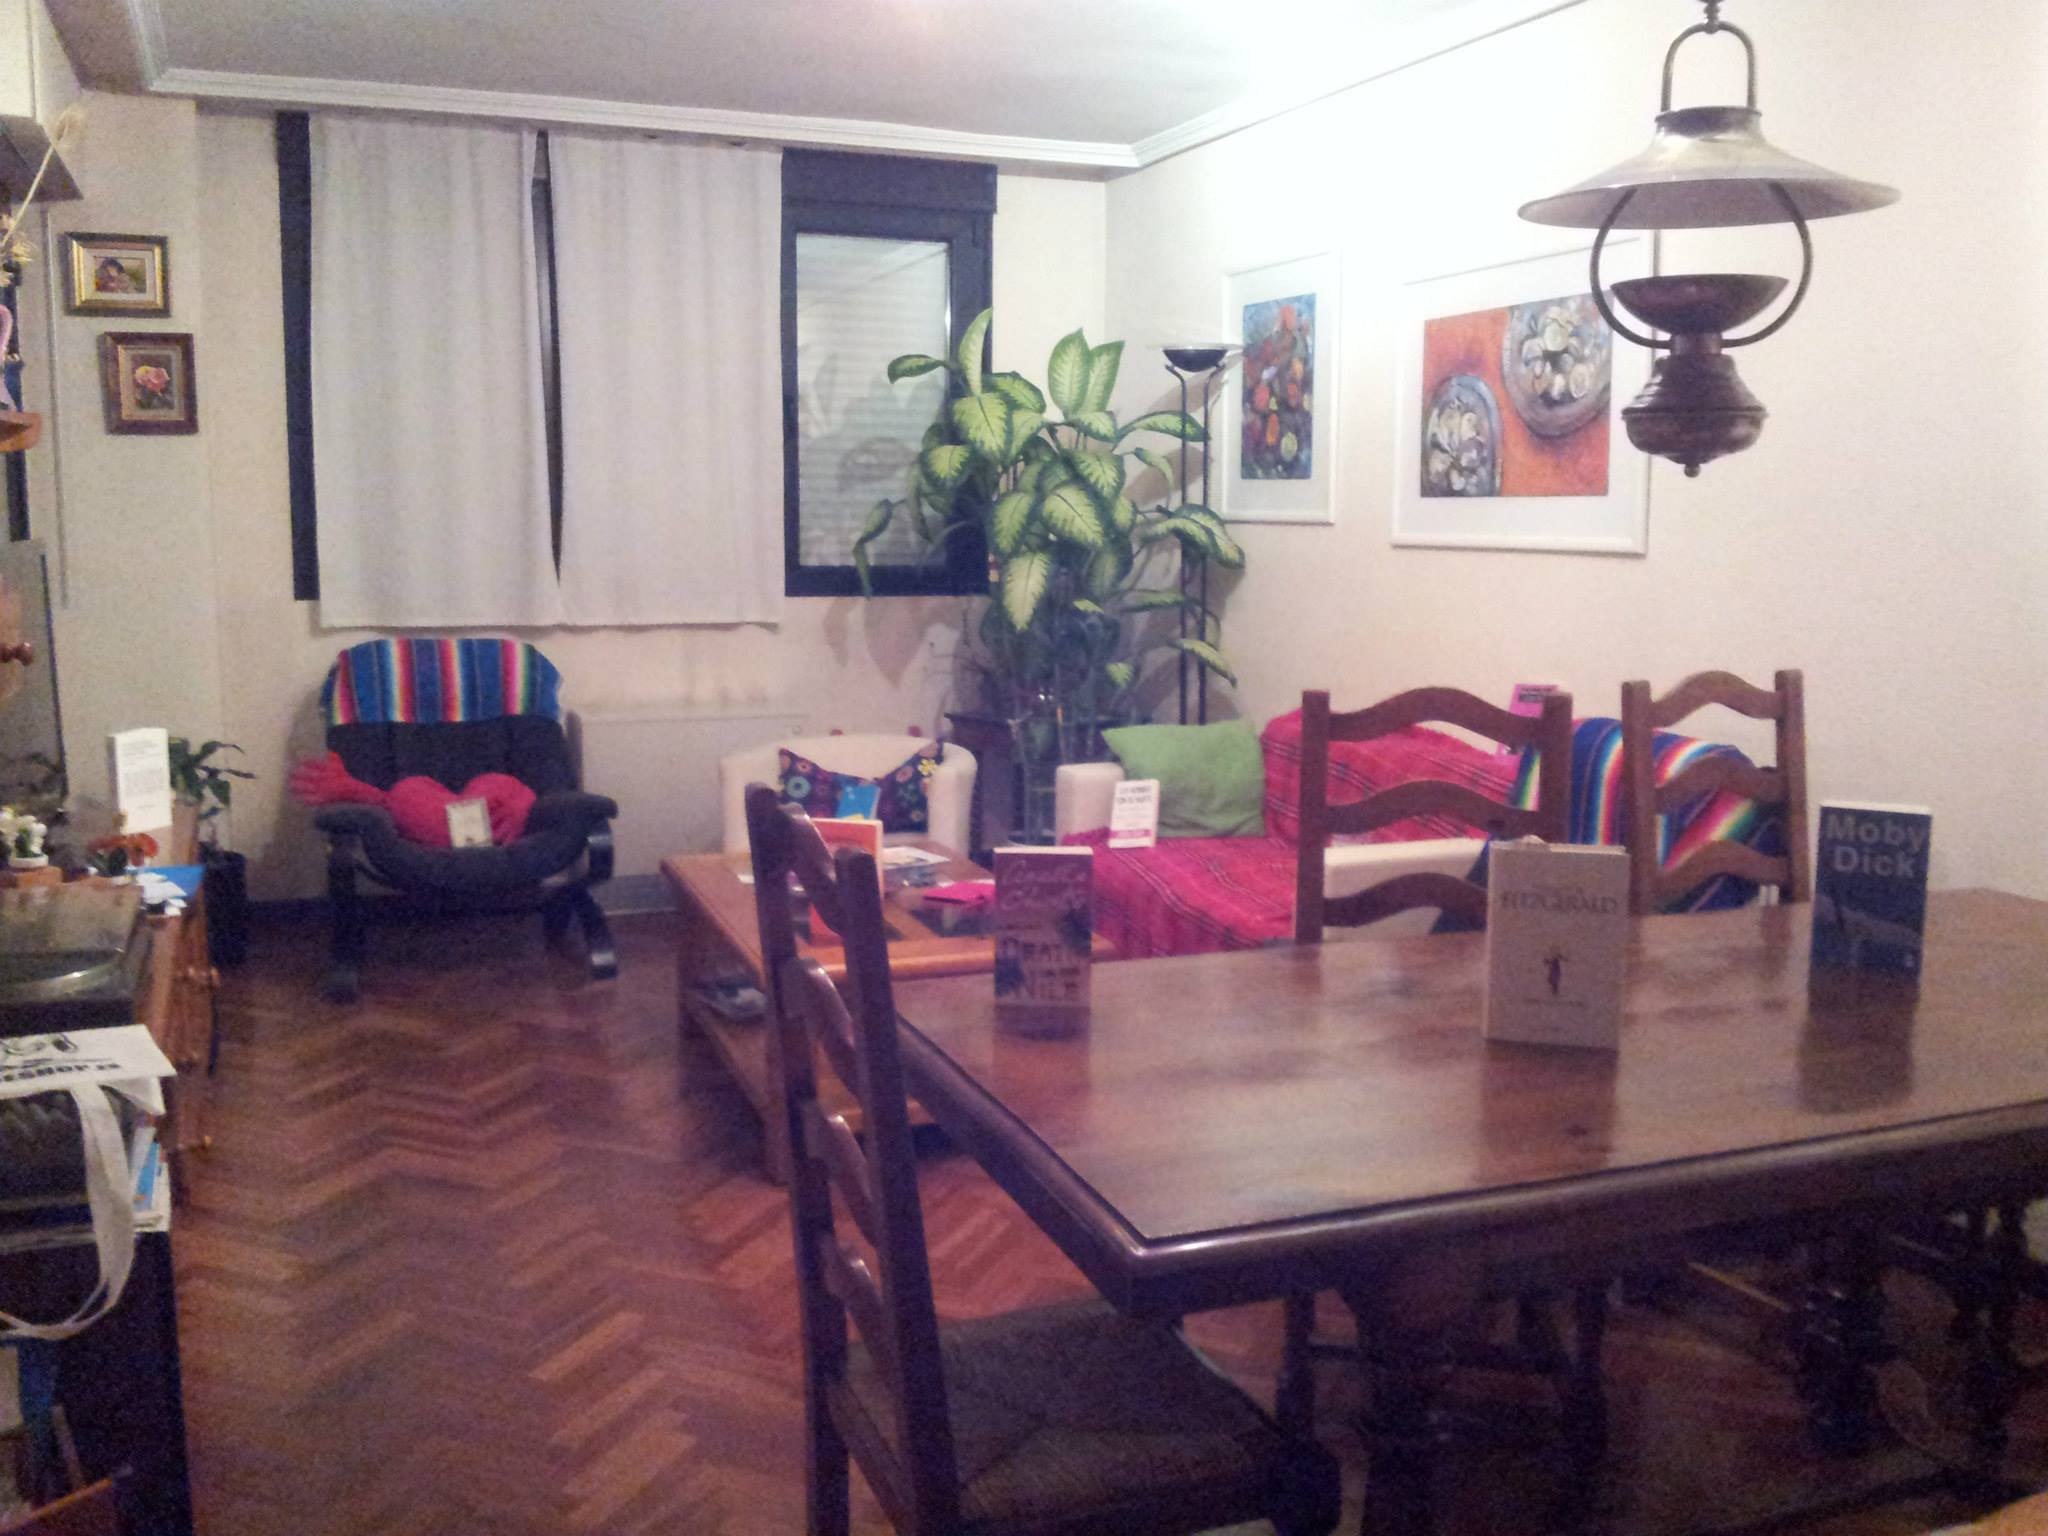
\includegraphics[width=0.75\linewidth]{images/2014/living} 

}

\caption{*Valladolid (Spain), January, 2014*: The 6th. [The *Three Magic Kings* night](https://www.donquijote.org/spanish-culture/holidays/the-three-kings/). There were no gifts at my house that night, so I picked up several books around the house and place them on the living room.}\label{fig:living}
\end{figure}

\hypertarget{totomas20140119}{%
\section*{2014-01-19 To T.}\label{totomas20140119}}
\addcontentsline{toc}{section}{2014-01-19 To T.}

Hello T.,

I know this is going to look like a draft, I'm sorry. It is what it is.

I'm writing to you in a hurry. It's the exam period. So forgive me for the stumbling of words, ideas and forms.

I just want to tell you that this is the first letter of many more that will come in the future.

I discovered the puzzle piece that didn't fit. The computer, the Internet. I was completely trapped by technology. I had to give all my tech gadgets to a roommate so I could study at ease and calmly. I promise you it's been one of the most liberating experiences of my life.

I am extremely comfortable and very focused, and I notice that I take much more advantage of the time. I'll explain the more detailed experience in the future.

These days have been very fruitful. I have a lot of projects and ideas that I'm jotting down as they appear in my mind. At the same time, I am moving forward with my studies at an incredible speed and with incredible efficiency.

I read an article about positive emotions that deserves a letter apart \citep{fredrickson2001role}. I'm much better.

Now I have to ask for your help, T..

I want to share this experience with the world and influence them so that people can experience this technological liberation. To be able to produce and create. I know there are a lot of people with the same problem as me, but some of them know it and some don't. But we're stuck in this tech network. A lot of untapped potentials.

I write to you with tears of passion, pain, and joy. T., I have a plan, an idea, a project. I can, we can make this change. But I need you to confirm that I can count on your support. I need your enormous knowledge so that the project grows and people can develop and grow on their own.

I have named the project \href{https://desconectando-unplugging.blogspot.com}{``\emph{Do you really need it? Plug off. Handwriting.}''}(Later, it came to my mind, ``\emph{Does it really matter?}'') ``\emph{Do you really need it? Does it really matter? Disconnected. Write by hand.}'' I don't know if \emph{Plug off} is correct or not, I didn't check it because I was disconnected. I'm not going to do it now, that I have internet access and I could, because I have to study for exams. More than 4 days writing \emph{Plug off} in numerous sheets and I do not know if it is right or wrong. Best of all, I don't care. The idea grows and its content and details are a matter of science, which will be solved later.

T., I will work and sort ideas, exposing them with calm, order and coherence. I have some doubts in some respects that I will expose you. But for now, I'd just like to know if I can count on you.

I hope you're doing all right. I'd like to hear from you. But until the 29th I can't give you the time you deserve. I am sorry.

From 1 to 10, I will be in Morocco, so the letters and the project will be delayed a few days.

A huge, excited hug,

Carlos

\begin{figure}

{\centering 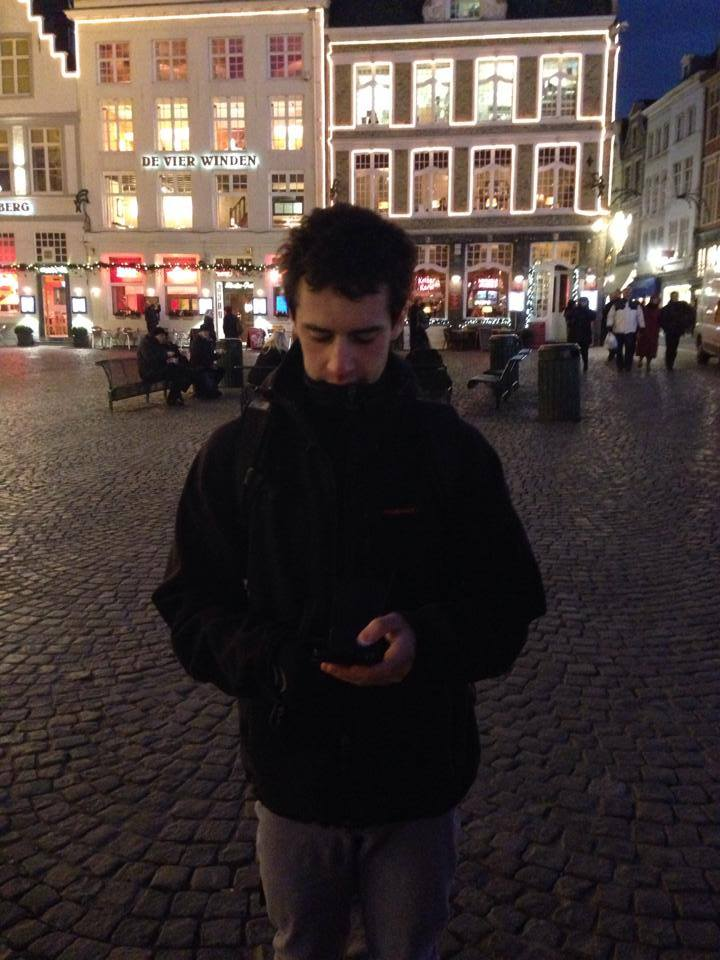
\includegraphics[width=0.75\linewidth]{images/2014/smartphone} 

}

\caption{*Brugges (Belgium), December, 2013*: Black Mirror's victim was about getting liberated.}\label{fig:smartphone}
\end{figure}

\hypertarget{reconnect}{%
\chapter*{The re-connection (January - March)}\label{reconnect}}
\addcontentsline{toc}{chapter}{The re-connection (January - March)}

\begin{figure}

{\centering 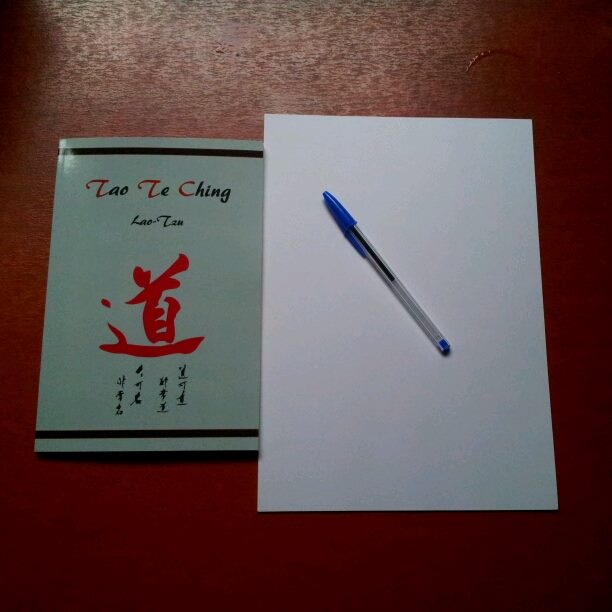
\includegraphics[width=0.75\linewidth]{images/2014/tao} 

}

\caption{*Leuven (Belgium), March, 2014*: It had happened, and it was going to keep happening.}\label{fig:tao}
\end{figure}

\hypertarget{frompaloma20140211}{%
\section*{2014-02-11 From P.}\label{frompaloma20140211}}
\addcontentsline{toc}{section}{2014-02-11 From P.}

Hello Carlos, how's it going?

The missing one\ldots{} I guess you've been traveling, haven't you? Morocco, isn't it?? Ui, ui, that healthy envy. Surely it has been an experience, tell me things.

I'm going to Bristol this week to see some friends and see if I can disconnect a little. What's that about you losing your phone? I hope that you solve it soon. You are such a mess!!

Well, how were the exams? I suppose fucking nicely or at least well. You're probably already handling yourself speaking English very very well, Manuel. Hahahahahaha. And what plans do you have for this quarter??

I've finished the exams and I did nice although I haven't yet been given the psychosocial mark. They're so slow. And nothing\ldots{} All subjects pass and that. Although I am aiming for more. Now starting the next quarter and I think that the party is gonna be over\ldots{} Many assignments and many classes to which I have to go necessarily. In fact, right now, I am in ``\emph{Psychology of personality}'', and it seems to me that participation and ass-kissing count more than anything else. Hahaha. I also wanted to ask you for an opinion on how to work on the subjects and all that, and which are themost interesting and so on. But well, you will tell me if you remember. I have: personality, critical thinking, health, linguistic and cognitive development, and psychological evaluation. When you can and feel like it, you tell me what you want. I relied too much on your advice that has always been good for me.

Regarding my life, not so much novelty: living in Salamanca and disconnected a little bit from my life from before, honestly\ldots{} I want to do new thingsssss!!!! So that's what I tell youuu. I hope you enjoy the quarter and we talk soon, ok? Be happy!!

A huge kiss, freak!

\hypertarget{topaloma20140211}{%
\section*{2014-02-11 To P.}\label{topaloma20140211}}
\addcontentsline{toc}{section}{2014-02-11 To P.}

Hello P.,

I'm all very well. I arrived yesterday from Morocco. A fantastic experience. I'm writing a chronicle of the trip, so when I finish it I will send it to you so that you give me your opinion before posting it on the blog.

When you travel, open your eyes, talk to people, ask them the most basic and absurd thing you can think of. The world is full of nuances to taste. Leave your phone in airplane mode during the day. Enjoy the moment. Others can wait for a while for them to know how you're doing. Take pictures of everything that deserves a photo. Good pictures, you know how to take them. But leave the best moments for your memory. Don't photograph those.

The stars of the Sahara sky cannot be photographed with the smartphone. The sunset on the mountainous horizon while I was meditating/praying on a dune, can't be photographed either. I got goosebumps every time I think about it.

If you really want to disconnect, don't worry about others. Your time is yours. You can tell them you're going to be out there and when you get back, you'll let them know.

The cell phone has appeared. It's at Charleroi Airport. It's 20€ transport to go back and forth. So, I will see if I can find someone who can pick it up for me. It makes me think it showed up. I think a lot about how I have behaves in the past with the goods that didn't belong to me. I need time to think about that\ldots{}

My grades are given to me on the 13th of February. Everything went pretty good. I'll tell you when I know numerically. English works in ups and downs, oscillating.

Plans for the quarter: too many. But at least I'm getting used to not using the computer/smartphone, writing by hand and sleeping less than six hours. We will see what are the results\ldots{}

Don't use your smartphone/computer when you're in class. Look at the professor's face. They will have already explained to you how important feedback is at this point. Live in the moment. Technology is a tool, not a part of you. You don't go with a hammer to class and you start hitting the table. Even if you can. Every tool has its moment. Control the tool so the tool won't control you. Look with your eyes and think with your brain. Write with your hands.

About the subjects of this quarter.

Personality. I got a distinction with honors. It's true it's about ``ass-kissing''. Interest, curiosity, participation are prettier words, though. Palenzuela is a pretty active, nocturnal person, like me. We got and get along pretty well. He's not the best teacher, he gets messy with the ideas quite often. But it makes you think twice as much, so you can build on your own what he means. Take it as a challenge, not as a threat.

Critical thinking. I did almost every assignment with an incredibly hard-working girl. She did most of them. Read the book and take it as a guide. It's all there. Silvia was my teacher. Very friendly, nice and accessible. We got along very well.

Health. G. also gets messy by himself. Sometimes he explains things in one practice group that he doesn't explain in another. Compare your notes with people from other groups and take lots of notes in the theoretical class. He knows a lot. If you're interested, ask questions. However, well, it's clinical psychology, and it wasn't my favorite subject.

Evaluation. If C. G. is your teacher, go to class and copy everything she says. Looks like a dictation. It's kind of ridiculous for a university class, but it's what he asks on the exam. Go to the practice class. If it Genaro is not your teacher, I have no idea.

Cognitive development. Read the articles before you go to class. Go to the library one afternoon, no phone or computer. Take a couple of hours to read it. You're going to make the most of the class and save time in May. The work is long and tiresome. Try to anticipate and get it done with time. It's pretty methodical, so you don't have to think too much, but you have to work a lot. It takes time.

Live the present, P.. Quit technology and meet people. You don't tell everyone everything you do. Write something for yourself. Handwrite. Do things one at a time. Focus on what you're doing and forget problems you can't fix right now. Note them up so you won't forget about them and you'll fix them in the future. Learn and let yourself be influenced. Don't prejudge, as much as it is possible. You're smart enough to make your decisions on your own. But if you need help, ask for it. Always.

We're in touch, P..

I also attach to you the work I did in Personality. It's two pages. Pa. quite liked it, so you can trust it to be fine. But he'll remember, so don't copy it. I hope it will guide you. Don't get stuck with the writing question. Read it slowly, and if you don't understand something it's normal. You haven't studied it yet. I think the terms ``personality process'' and ``personality in action'' are reversed. That's what he corrected when I gave it to him. Personality in action is the operation of the personality in process and the personality state is the result of the personality process. Don't trust me too much, wait for May. When you read it again everything will make more sense and you can correct my work.

A kiss,

Carlos.

\hypertarget{tot20140217}{%
\section*{2014-02-17 To T.}\label{tot20140217}}
\addcontentsline{toc}{section}{2014-02-17 To T.}

Hello T.

Today I feel a little tired, I suppose it is because it is already night, my throat hurts and I am considering taking some caffeine or going to rest.

I am writing to you briefly to tell you about my ``successful'' completion of the first semester as an Erasmus. At least academically. All passed.

\begin{figure}

{\centering 
\includegraphics[width=0.75\linewidth]{images/2014/study} 

}

\caption{*Valladolid (Spain), December, 2013*: I successfully passed the exams thanks to long study sessions in the library like this one.}\label{fig:study}
\end{figure}

In general, I am in quite a good mood and I have taken this past week to organize my schedule and prioritize my projects. Re-adapting to student life after my trip to Morocco. (There is a chronicle of the journey in hand; hands paralyzed unfortunately \ldots)\footnote{6 years of paralysis already.} Still, I think I want to do too much and often go overwhelmed. I plan to write down a motivating message about the difference between moments of inspiration and day-to-day work. Maybe it will work. I'm not sure how to carry out everything I want. I have a schedule with almost no breaks, it is somewhat unreal\ldots{} In moments of euphoria I write down my ideas and fit them into non-existent hours throughout the week.

I would also like to write more (I have noted down to write at least once a day, either reflectively or communicatively, like right now). With the subject of writing many times it is the first impulse to start writing what I lack. If you have any advice on how to remedy that primordial spark, I would really appreciate it.

Anyway, let's stop egocentric banalities. I would like to know about you, your family and your projects.

I hope everything is going well.

An affectionate hug and thanks for your time.

Carlos

\hypertarget{tolucia20140220}{%
\section*{2014-02-20 To L.}\label{tolucia20140220}}
\addcontentsline{toc}{section}{2014-02-20 To L.}

\begin{quote}
it went off

she is not here

she is not now and she has not been

she could be dead right now

or have been

you were talking with pixels

with a screen

it was a recording

in its due time

time
\end{quote}

Hi L.,

The phone just went off and I wanted to continue talking to you. For this reason, I am writing (by hand, obviously).

The first thing that came to mind was the verses you just read. That is why they are the first written thing, it is a reliable and chronological representation of the handwritten sheet of paper.

At the time the phone was turned off, I was close to feeling anxiety and concern that I could not continue talking to you. But now I'm doing it. I feel like I'm communicating with you. I feel better. I have simply had to overcome the first instinct of inactivity or search for technological contact with you. I have started writing.

Even if I am writing this letter at night, you may read it tomorrow, in a week, or in a month. When I want to send it to you, if I send it to you. You may reread it in years and each time it will be different for you. You will be able to read this letter if I die before you and it will appear that I am speaking to you. (This is how I just beat death. This letter is my song \ldots{} (Tweet in English. Food for thought, isn't it?))

Poetic parenthesis.

\begin{quote}
\ldots{} And I will leave. And the birds will stay

singing;

and my garden will remain, with its green tree,

and with its white well.

Every afternoon the sky will be blue and placid;

and they will play, as they are playing this afternoon,

the bells of the bell tower.

Those who loved me will die;

and the town will become new every year;

and in the corner, that of my flowery and whitewashed garden.

my spirit will wander, nostalgic \ldots{}

And I will go away; and I'll be alone, homeless, treeless

green, without white well,

without blue and placid sky \ldots{}

And the birds will stay, singing.
\end{quote}

\begin{quote}
Wild poems (1910-1911). \href{https://en.wikipedia.org/wiki/Juan_Ram\%C3\%B3n_Jim\%C3\%A9nez}{Juan Ramón Jiménez}. \citep{jimenez1970tercera}
\end{quote}

This is what technology has demolished. Haste has wiped out patience. The wait, the tasting of the moment, the pleasure of the non-immediate \ldots{} The enjoyment of one's own personality, of internal communication. Ultimately, life itself.

I don't want to continue writing, so you start doing it. But this little letter/reflection is clear proof of the benefits of writing and the harmfulness of digitized communication. In a few lines and almost without arguments.

Now, I start reading. I'm much more relaxed than I was five minutes ago when the phone went off. Also, writing this seems much more real to me than sending you a WhatsApp : ``* I'm fine*''. Although it will take days, hours or years to send it to you, or you to read it, for me it has been much more immediate than a WhatsApp.

Good night.

A huge hug.

P.S. You know I would like to hear from you. (General and extremely open question that you can answer with the degree of detail and specificity that you want). If you want to just write to me that you are fine, I will believe it and continue my life placidly. Taking advantage of my time knowing that L. is happy. Lying to me is lying to yourself.

\hypertarget{tos20140221}{%
\section*{2014-02-21 To S.}\label{tos20140221}}
\addcontentsline{toc}{section}{2014-02-21 To S.}

2014-02-21

S.,

Patience is a really beautiful virtue that gets corrupted by the abuses of technology. Sincerity is the delicious fruit of patience.

You asked me a few weeks ago how I was doing, and I replied that at that time I did not have time to respond adequately, that I would write to you in the future. That future is today. I consider that it is a good moment to tell you a little about how I am.

I couldn't answer you when you asked me because I didn't have enough time. Also, I was not comfortable answering you in a hurry and without the care and detail that you deserve, and I deserve. I hope it hasn't arrived bad and that you understand it. I like to take care of communication. I am willing to sacrifice speed for quality. So, I hope your answer, if any, is not hasty. Make it honest, of high-quality. I don't care how long it takes you to write to me, it can be two days, or it can be two years. I'll be fine.

In these moments I am very happy. I am very comfortable with my life. I am flourishing, I am incredibly productive. As I never have been. I am learning a lot: I read, I write, I meet incredible people, who show me new horizons and expand my mind; I tear down walls of the past; I understand part of the numerous mistakes I made in the past. But I don't blame myself. Those mistakes are part of my life, of my learning, of being where I am today. I needed to make a mistake to get where I got to. Sometimes it was necessary to be wrong once, but other times it was necessary to be wrong again and again. Enough times until I learned. Many of my mistakes have revolved around you. It had to be this way to learn. If they happen again, it will be equally necessary. It will be proof that I have not yet learned what I have to learn, that I have to continue learning.

Now I am understanding countless things that were incomprehensible to me in the past. That, at times, I acted in a completely illogical, extremely passionate way. Many times, in a hurry and worried about the ephemerality of the moment.

Now I'm calm. Much calmer.

In these moments of inner calm, few external storms can stir my spirit.

S., I would like to hear from you. You are a person whom, I feel, I have not treated as you deserve. I can learn a lot from you, and I have a feeling that we could have an incredibly fruitful relationship for both of us. No matter the physical distance, as long as there is a spiritual, intellectual, and / or emotional union. The power of the non-physical knows no limits in time or space. (Imagine reading this letter and that I am dead. You could still answer it and be communicating with me.)

Out of respect; towards me, but much more important, out of respect for you; I hope you will give me a thought worthy of your ability. If you lie to me, you are lying to yourself. I wrote a couple of days ago to a friend, who told me to that she was ``\emph{fine}''. Personally, I highly doubt it. So, if that is not true, there is nothing I can do as a friend to help her. But, much more damaging, for both of them, I will believe that there is nothing wrong in not helping her. Lying to me is lying to yourself.

I would like you to answer me, please. Slowly and sincerely. If you do not want to answer me, I perfectly respect your decision.

Carlos

\begin{figure}

{\centering 
\includegraphics[width=0.75\linewidth]{images/2014/glove} 

}

\caption{*Brussels (Belgium), November, 2013*: Taking out a glove to take a selfie. Very smart behavior in Northen Europe.}\label{fig:glove}
\end{figure}

\hypertarget{fromT20140222}{%
\section*{2014-02-22 From T.}\label{fromT20140222}}
\addcontentsline{toc}{section}{2014-02-22 From T.}

2014-02-22

Carlos, good morning.

Congratulations!! For that first term that you have passed as a good Erasmus, not as some have led us to believe that you were, Erasmus students \ldots{} Not even Flemish has been a problem, from what I see, which means that you have jumped into the pool since the first day, without fear of the waters and their turbulence.

Do not think I have many things to tell that you do not know or suppose. These last days, and I am going to continue like this until the writing of the paper is finished, I have dedicated the whole time to \href{https://en.wikipedia.org/wiki/Gottfried_Wilhelm_Leibniz}{Leibniz} or, more specifically, to deepen the \href{https://en.wikipedia.org/wiki/Th\%C3\%A9odic\%C3\%A9e}{conception of the will of God} in Leibniz and in the government of the world. There I am, rummaging, with the magnifying glass on - and even the microscope -, alone with his texts, basting ideas and asking questions. I have gone from having things half clear to clarify myself conceptually, but to see how doubts grow in me about Leibniz himself and his philosophical environments. Right now, although I think I will not raise it in the congress - perhaps I can only point something - I have more and more doubts about the concept of God in Leibniz and in modern philosophy and, through them, about metaphysics, to which I still consider it a fundamental discipline, but whose content depends excessively on the medieval tradition. I leave it there, because you cannot walk with hypotheses and doubts.

Your lack of time - and everyone's - is typical of our time and I am afraid it has been the fate of all the intellectuals who have populated the earth. In any case, in this time of weak, mercantile thought, lost amidst the superficiality of appearance, of manipulations everywhere, of manipulative and adolescent media, of \emph{palabreros, truhanes, mercachifles}, in short, cynics; at this time, to the obligations and commitments of studies and knowledge, we usually combine the time-eater media, which dilute our time, the ability to think, manipulate us and even shape our moral conscience. In the face of all this - the liquid society that \href{https://en.wikipedia.org/wiki/Zygmunt_Bauman}{Bauman} talks about - one must select a great deal and be faithful to the schedules that one has drawn up. \citep{bauman2013liquid} Liquid society liquidates\ldots{} In other words, when you set timetables and follow them, you are on the right track. We usually fall, I have been, and I am a victim of this, in the temptation to peck at everything, which in the end leads us to delve little or nothing into almost nothing. If it works for you, you who are young can avoid the defects into which many have fallen.

There I continue with the essay reading workshop and forcibly committed to the Parkinson's association, which is taking me much longer than I thought and wanted. At the moment, I have written the contents of the new website, which are mainly medical content, I have already visited a good number of official offices begging, as they say. You go into offices that have plenty of luxury to ask for something that is fair and whose responsibility is the administration, because those affected by Parkinson's have to finance their therapies themselves, since Social Security washes their hands with them. But these sick people are there, with a degenerative disease that lacks a cure. Very strong, but real. They even have the association in some premises, an apartment on a ground floor, which some nuns have left for them. We are fighting there. Let's see what we get. Look! The association is thirteen years old. I have my brother-in-law affected by Parkinson's, who has had to take the presidency of the association, because they had led it to bankruptcy due to mismanagement and the malfunction - I am going to leave it only there - of some worker, especially the psychologist, who until now have not dared to put her on the street, as I think they should. As you see, I walk everywhere, but not as God but lost in what unknown worlds\ldots{}

Well, Carlos, you do your thing. Learn in someone else's head, in the head of those who, like me, lose themselves by multidisciplinarity - how good I am with myself! - and do not just ``squeeze'', as the saying goes, in nothing. It is very important to delimit the territory well, since it will be life - the circumstances, \href{https://en.wikipedia.org/wiki/Jos\%C3\%A9_Ortega_y_Gasset}{Ortega} would say -- who will invite and even force you to dispersion.

I'm going to see if I practice a bit in the kitchen now \ldots{} and surprise the family with something, although I don't know with what \ldots{}

Health, peace and happiness.

\begin{enumerate}
\def\labelenumi{\Alph{enumi}.}
\setcounter{enumi}{19}
\item
\end{enumerate}

February 22, 2014

PS: I have made sea bass with a mushroom sauce. Well, it didn't go wrong \ldots{}

\hypertarget{toLa20140224}{%
\section*{2014-02-24 To La.}\label{toLa20140224}}
\addcontentsline{toc}{section}{2014-02-24 To La.}

2014-02-24

Hello La.,

I know you live in Leuven and I know face-to-face, oral communication, it's invaluable. Still, I wish we could write to each other quite frequently. Of course, the social and emotional nature of our relationship will be maintained face-to-face but debating more purely intellectual content with you in writing can be very fruitful for both of us. I think it will be useful to clarify some of the ideas that we have put forward in recent days.

There is a possibility that you may not have time to write. I understand that writing is patience and not rush, so I don't mind if your response is delayed if the quality deserves it. New technologies are in a hurry. Haste produces mistakes and stumbles. With what, ironically, in the long term, cause waste of time. On the other hand, I consider that by using writing continuously, cognitive processes are streamlined, and time ends up being gained.

For this reason, I sincerely ask you to dedicate a part of your day and your time to disconnect the distant-communication devices of your room, mainly mobile phone and computer. Then, you can write without interruption and concentration, by hand and from memory. Without data or unnecessary references at the time of the original creation of written thought.

The first question I would like to ask you is (assuming your extensive knowledge of, among other things, linguistics) whether you could expose to me the most important differences between the written word and the spoken one. In order not to overflow us with the size of such a question, which I suppose has originated countless books throughout history, I ask that you please do not exceed 2 or 3 pages. For you and for me. Try to condense everything that reflection allows you. To encourage your intrinsic motivation, you can take it as a great summary of everything you have learned so far related to this topic.

I hope to receive your reply soon.

A warm (and not intellectual) hug,

Carlos

P.S. If you want, you can take the opportunity to correct grammar, spelling and punctuation errors, among others.

\hypertarget{fromLa20140224}{%
\section*{2014-02-24 From L.}\label{fromLa20140224}}
\addcontentsline{toc}{section}{2014-02-24 From L.}

2014-02-24

Good morning, good afternoon or good night.

Today I start writing without knowing the day I will finish. I want to emphasize that, at this very moment, the time I am using to write this letter should be used for other priority reasons. However, today I feel like thinking and writing.

I think the time here is consumed vertiginously, which makes me dread. The embarrassment unnerves and weakens me. I need to plant time and thus collect hours with fruits. Incurring in relatively ``absurd time-killers'' may not be a good option, given that I regret my limited time. I want to achieve a greater deepening and internalization of the university contents to acquire.

I admit that the commitment that I have guaranteed in the scout group in which I have signed up, is not in accordance with my real ``free'' time, which dissipates or evaporates an excessively necessary time. I may not be mature enough to deny proposals (both from friends and the group). Maybe I shouldn't be securing projects that I can't commit to.

The other day they called me something between ``hypocritical and false'' at the same time for this very reason. I don't have the capacity to deny a purpose that they make me. It seems like wanting to give 100, without sometimes being able to reach 50. This is how I end up doing it: badly, in a hurry and running. Still, I step back, stop, and think. Organization is the solution, or maybe the first remedy is to learn to say no?

You who seem to know me, tell me what you consider. Today, I let you be what you like to be.

Greetings Dr.~Alcalá,

\hypertarget{fromL20140224}{%
\section*{2014-02-24 From L. to herself}\label{fromL20140224}}
\addcontentsline{toc}{section}{2014-02-24 From L. to herself}

2014-02-24

01/22/2014

Dear future ME:

Who would know about my today self in my past and how funny period I have put her through. The past me has not had a good period years ago, but this year, the proposed objectives have been set. Maybe I wouldn't have thought I'd get here, but hey, you did it!

You study dance, your life is dance. Today is not too late to improve and train yourself. You can become better than you were yesterday. (And so much compared to your younger years.) I should scold you for too much letting yourself go in your crazy adolescence, since today I regret such a time. However, one writer told me not to be afraid of being the person I have become. That one should not be discouraged by the wrong decisions one made. I must trust my old self. Maybe my thirteen-year-old self could have been mistaken for not studying enough or for being too carried away with that high school boy. But it was I who made the decisions and surely spent some time making them.

Why do you think you now have the right to judge what she (your old self) decided? Accept who you are, don't be afraid to be the person you have become with your decisions. Bad decisions weather, bad decisions, in time, will be good decisions. Accept that and you will be very happy in life and, above all, with yourself. About 80\%, you are a consequence of your decisions. Love yourself for the result of what you are. Love yourself because that is what you have become. And above all, recognize that sometimes you are wrong. And that 20\% of mistakes, you have to recognize and accept them. It is important that we recognize that we are wrong in order to become aware of where the errors are and not make them anymore. Perhaps many are afraid of the punishment that this can entail, but the punishment is the least of it, the only important thing is to give our brains the correct items.

Maybe without those years, you would not be what you are today.

However, look at where you have arrived. University? At what point did it cross your mind the idea of not-trying it?

Remind you of our family, you should spend more time with them. They have given you everything, today give for them. Love them more, show them more. You are their fruit, do not regret it. (Although I must add that it would be good if you boost trust and interact with them, I consider it essential for your good communication.)

I think that the greatest significance that there has been in my history has been thanks to friendships that I have been collecting over time. (Someday I will write to them). Most are old ones, from always, many others were passing by and wanted to stay awhile. They are surreal stories, but they are the ones that are recorded in mind and skin. They are part of your past, present and expected future self. They are the base, your bases and your being. They complement you. Who would you be if not? You collect bits and form yourself; but not only with them. Today they have marked you and you are what you are for them.

I think you should also be grateful every day for the tortilla turns that they gave you one summer, maybe you weren't here today if it weren't for those.

Keep all your memoirs, memories and moments. Today you are, because you were yesterday.

Value yourself, love yourself. They already do, now only you are left. I am already working on it.

Tomorrow, I hope this makes you think, and you like it. Until then, I look forward to great achievements. I think your time has come to take advantage of the untapped. And what the hell, you're in Madrid! Thousands of affairs, to a metro subscription. You know, your time has come. I hope you have gone as far as I want today, and if you have gone further, the better.

LOVES YOU,

Your previous self

\hypertarget{tomother20140224}{%
\section*{2014-02-24 To my mother.}\label{tomother20140224}}
\addcontentsline{toc}{section}{2014-02-24 To my mother.}

2014-02-24

Hello mother,

You have worked for a fairly long time of your life, and now you have free time and money. With what you have right now, you have the necessary factors to go on a trip. Having a child abroad, you have the perfect excuse to spend some time in Belgium.

Come to Leuven to spend a few days with me, mother. I am in a moment in which I spread peace, happiness and calm around me. A few days here may be perfect for you. We both know that you love to travel, see the world, learn and have new experiences. I think I can guarantee that your time here will not be wasted. The only objective I have with your visit is to learn and that you learn everything that you have taught me.

I can affirm that you are a perfectly independent person, with the necessary skills to operate freely in Belgium and Europe. Don't worry about me, I will take my time to do whatever I need or want, if I need or want it. So, I would not like you to think that you can be a nuisance, annoyance, or a burden. Don't worry about me: I know hoe my mother is like and I know I won't have to take too much care of her. ;-)

Personally, I have the feeling of showing my gratitude and being thankful for everything you have taught me. But I don't know when or how often I will return to Valladolid, (Spain). The opportunity of continuing learning from you while giving back part of everything you have given me may not come easily. It seems to me that right now is the right time. I would like to spend as much time as possible with you in these moments, because in the future I do not know the distance that will separate us nor the ease and frequency of our meetings.

Since I don't want you to spend excessive money to come here, we can talk about different possibilities. As for the accommodation and other amenities, don't worry, you can sleep in my room and I can go to a friend's house. Or we can sleep, if you want, the two of us in the same room. We will be deciding by sharing our points of view.

``\emph{You have to go empty to return full. You have to go back empty, to fill yourself}''. At the moment, neither you nor I know how to do it, but we try to learn enough to make it happen.

A warm and comforting hug,

Carlos

\hypertarget{frommother20140225}{%
\section*{2014-02-25 From my mother.}\label{frommother20140225}}
\addcontentsline{toc}{section}{2014-02-25 From my mother.}

2014-02-25

Hello, dear Carlos.

I greatly appreciate your letter and the encouragement that conveys and comforts me.

I am glad you are in such a plethoric moment, of well-being and happiness, with high expectations on the way to achievement. I am also encouraged to know that the small or great efforts we have been able to make for you and for your brothers have served you; that they have transmitted you knowledge and experiences; above all, I hope, of affection, emotion and love -which, on the other hand, it costs me so much to show sine a few years-; I hope that the moments lived during the first years of childhood and happiness weigh more.

Your offer fills me with satisfaction and I am sure that those days with you would be, as you say, of benefit, rest, and perfect for my state of mind, and, thus, be able to appreciate the many things that have been going through my mind lately. I agree with what you tell me and you propose -I think it is the right/necessary time and although it may serve as an excuse I would never feel like this-, I would love to take that trip and share with you the moments that your daily activity allows you, and your room , that you do not have to leave for me, with a sleeping bag I have enough. But it is possible that this is not the time, I went this morning to a selection test for an Ecyl teaching course, which I have wanted to do for years and I have the interview on the afternoon of the 27\textsuperscript{th}. Until that moment, or one day later, I will not be able to seriously consider the trip, which causes a small conflict of interest, as I would undoubtedly prefer to be with you, but if I were selected it would be a great opportunity that I should not miss. We will see.

On the other hand, there is one more inconvenience. Your brothers have not finished the course they are doing and your father is working, things that morally bind me to this place, although it is not a great thing that I do for them, which on the other hand I do not feel be recognized, requested, or claimed.

In addition, you already know your father and his economical ideas, that so many inconsistencies and inconveniences pose to me in day to day and coexistence, not only with him, especially with you and in relation to my family. Something that would not pose any inconvenience, or doubt, if you really needed my help and/or presence.

I thank you very much for the effort and time you dedicate to me, especially when you are so busy, and the recognition or feeling of gratitude that you transmit, of positive value for what we do or try. And although I would like to have you close - you know that it really lasts little when you are physically- what really comforts me is that you are growing and achieving what you are interested in and you propose and what your future reward means. The disadvantage of distance is bearable when you see and value the benefit it provides, even if it is not always easy to accept or carry.

We continue in communication, accompanying ourselves in the search for the best, in continuous learning, on a daily basis, in the experiences of ``emptying and fullness''.

A warm and comforting hug.

Estrella

\hypertarget{toC20140225}{%
\section*{2014-02-25 To C.}\label{toC20140225}}
\addcontentsline{toc}{section}{2014-02-25 To C.}

2014-02-25

Hello C.,

We haven't talked in a while and I'd like to hear from you. (General and extremely open question that you can answer with the degree of detail and specificity that you want).

Please, if you find some time, I would appreciate it if you could write me a letter (by hand) and then send it to me by mail in an attached Word document. You can tell me how you are, how your studies are progressing or how you feel your life is evolving.

I will be your most attentive reader. If you have any concern or doubt about a topic, you know that you can always count on some of my clumsy advice.

A big hug,

Carlos

\hypertarget{toCa20140226}{%
\section*{2014-02-26 To Ca.}\label{toCa20140226}}
\addcontentsline{toc}{section}{2014-02-26 To Ca.}

2014-02-26

Hi Ca.,

At last, I have found a moment to write to you. Something that I have wanted to do for quite some time.

First of all, I highly recommend reading \href{https://archive.org/details/flourishvisionar0000seli}{\emph{Flourish}} by \href{https://en.wikipedia.org/wiki/Martin_Seligman}{Martin Seligman} \citep{seligman2012flourish}. You should know that the book I recommend is not a self-help best seller, much less. Before making a criticism of positive psychology, you should bear in mind that the affirmations sustained in the book are methodologically obtained conclusions. Therefore, I consider the book of sufficient scientific validity to be respected. In this book, Seligman develops his \href{https://en.wikipedia.org/wiki/Martin_Seligman\#Well-being}{Theory of Well-Being}. According to this theory, one of the factors that directly influences individual well-being is positive interpersonal relationships. I consider our relationship as positive; and that is why I believe it is necessary to make the effort to maintain it, to improve the well-being of both. Yesterday I fully realized that the fundamental thing about human relations consists in giving and not asking or taking.

So, I'll start by giving you a little bit of me (apart from the book's recommendation):

In these moments of my life, I am very calm and at ease with myself. Today, for example, I had an incredibly sociable and happy day. Full of well-being. I am being honest with myself, on a personal and spiritual level (I am reading the \href{https://en.wikipedia.org/wiki/Tao_Te_Ching}{Tao Te King} \citep{ta1984tao}. We will talk about the Tao in the future if we consider it necessary.

My use of technologies is gradually approaching what I consider to be correct and measured. I have found time to read, write, learn and maintain the relationships that really matter to me and bring me; at the same time, I meet people who are incredibly amazing.

In this letter I would like to write to you about some of the advantages of remote letter communication. I will focus more specifically on the advantages of written communication, leaving aside the subject of writing as a reflective element and support for thought. What I write below, I hope, is part of a larger, more detailed and refined reflection, which may become part of an essay. I want to polish and improve this thinking as much as possible, to give it a much more perfect shape in the future. Therefore, I also hope that you will detect my argumentative weaknesses and the possible conditional clauses necessary to refine my ideas.

I would like to underline the fact that I want to discuss this topic with you because of some of the conversations we had in the past, about oral and written communication; or the value of writing as a the little sister of thought and support of it.

I hope to be able to cover the topic of writing and thinking with you in the future, since you also demonstrated to have a quite formed position on it\footnote{Following I shared with C., my now \href{https://www.carlitofluitoideas.com/writing-letters/}{classical text about the advantages of writing letters}.}.

\begin{quote}
ADVANTAGES OF LONG-DISTANCE, NON-NSTANT WRITTEN COMMUNICATION (BY LETTER) \footnote{Original post in Spanish published here.}.

There are some characteristics of written, non-immediate communication (by mail) that I consider advantages. Next, I will highlight some of them.

Firstly, as an anecdotal fact, consider that written communication (by mail) has been the main, and practically the only, way of distant communication throughout long distances for most of our history as human beings. Moreover, some of the greatest thinkers have left us, as an essential sample of their thoughts, their epistolary texts with contemporary thinkers. In those letters, we can approach their thoughts and ideas, since writing offers an invaluable mechanism to transform a thought into something lasting and stable through time.

From a more affectionate and relational perspective, I want to highlight the true interest shown on someone when a letter is written to them. Just the act of sitting down and write implies a prioritization of the interpersonal relationship upon multiple other possibilities. In essence, a fair amount of personal and individual time is dedicated to the other person, as well as your almost full attention.

As proof, I am writing this text thinking about you right now. It feels as if I had you in front of me as if we were talking. I am dedicating my time and my attention entirely to you. My phone and my computer are shut down. {[}The original letter is hand-written, and it has suffered a process of digitalization and correction.{]} The reason to be hand-writing is to achieve a representation as pure and reliable as possible of my thoughts and feelings. Ultimately, to allow the flow of ideas and emotions subjected to minimal hindrance or modifications. This detail about handwriting seems essential to me in true long-distance communication. \footnote{2018-09-07, Erratum: We all change. I change. Nowadays, I type much more, and I sent most of my letters by email. I can elaborate on those aspects in a future post.}

Secondly, I want to emphasize the freedom that writing gives both the writer/transmitter and the receiver. In the case of the transmitter, it has the freedom of taking as much time as needed to think, ponder, manifest and revise the content and format of the message. Thanks to this reviewed writing, the likability that the receiver (the other person) is going to read the actual message that was intended to be transmitted augments, decreasing the chances of the receiver decoding the message incorrectly. Therefore, the writer or transmitter needs to dedicate time to use the language appropriately, choosing correctly, with care and moderation the words and sentences in which the message is going to be shared. I presume that, in this way, a fair amount of misunderstandings are avoided. Misunderstandings occur easily in both oral and instant-messaging communication. I wouldn't like to be interpreted as contrary to oral communication or instant messaging; since both of them are going to be discussed in future texts with calm, details, and nuances.

In connection with my previous thoughts, it would be easy to use, as a counterargument, the slowness of handwriting, as compared to other communication channels. Surprisingly, using the hand-written communication channel in long-distance relationships can actually save time, given the fact that it helps to avoid errors or mistakes that tend to appear in oral communication and instant messaging. The transmitter has the possibility of reading the message as many times without needing to involve the receiver. Due to the lack of an expected and immediate feedback, the transmitter also saves time, since it doesn't need a passive awaiting of an answer, but could dedicate this time to much more productive activities, such as sleeping.

Another advantage, directly related to this idea of freedom that writing gives, is the independence that both the transmitter and the receiver enjoy when their communication is based on hand-written letters. Let's use a reliable example: the moment when I'm writing this letter it's a bright day and I am in Leuven. But when you read it, it won't be necessary for you to be in Leuven or to be during the day. In fact, this freedom is so wide, that you could read this letter when and wherever you wanted to. When and wherever it suits you because it is already written. You don't even have to answer it afterward, you don't even need the transmitter to be alive to receive and decode the message. Besides, you could always recall this information whenever you needed it because it is already written. In addition to what has been previously mentioned, it is worth mentioning the incorruptibility of the message. In our particular case, with different time zones and locations that separate us, I find especially useful a hand-written communication channel. Personally, I believe that this particular characteristic of hand-written communication, the possibility of escaping the limits of time and space, places it in a privileged position when it comes to transmitting thoughts and ideas. The instantaneity of the communication, either oral or by instant messaging (WhatsApp, Facebook, Skype\ldots) doesn't grant any freedom neither to the transmitter, nor to the receiver: neither time to reflect upon their message, nor to use their spare time in different activities since they are both waiting for instant feedback from the other side.

For these reasons, non-instant communication is the most suitable when the content of the message is prioritized over the feedback of the receiver (which is very egoistic). In other words, Instant messaging prevails when the consequences and the utility of the message gain importance over the value of the content. The new technologies have made us come to believe that speed is more important than the message itself. They've confused us by making us rush, driving us to an incomprehensible superficiality in personal relationships. The new technologies of immediacy, that claim to save time are, in my opinion, those actually stealing it. In future texts, I 'll inquire deeply into this statement, sustained by different subordinate sentences.

As a closure to my argumentation, I'll expose a possible counterargument for the loss of spontaneity in interpersonal communication, or worse, the loss of spontaneity in the relationship between the transmitter and the receiver. I consider that this affirmation needs to be explained: I believe in written communication as a refinement and not as a loss of spontaneity. I do consider myself an active, vivacious and energetic person that treasures to a large extent the spontaneity of life. Written language could continue expressing a fair amount of this ``spontaneity of life'' despite the reflection and refinement attached to it. It is possible to deal with a minimal loss of this spontaneity at the expense of improving the expression and exposition of ideas. This is a price I am willing to pay. This way, we could concentrate this spontaneity in face-to-face relationships, which I consider fundamental for human beings' emotional well-being. But this kind of spontaneity that technologies are defending seems to be a cheap imitation of actual communication, that doesn't involve actual face-to-face spontaneity, neither reflection nor the refinement of expression that proper writing achieves.

All things considered, I defend non-instant, long-distance written communication (by letter or mail) is the most accurate communication channel to keep positive interpersonal relationships at a long distance. With letters, a true bonding and interest towards the other person are shown, alongside a search to deeply engage in the relationship; while using the new technologies from the immediacy era what is actually pursued is utilitarianism and superficiality in personal relationships, including also the telephone or video conferences. I believe that a connection made through shared written thoughts is more real, deeper and true than one created with on different colored pixels forming some image similar to a face on a screen and a robotic voice coming out of the speaker. Referring to sensations, I would rather look at a photograph (if printed, better) of me and a friend in some lost place in the world and then try to listen to his or her voice in my head while I read his words. Also, why the rush? What for? If you really care about keeping the relationship alive you ought to give some of your time exclusively to that person, stop and think of him or her and write them. This should be a clear proof of devotion and interest for the reader, and not any `How's going?' sent by Whatsapp.
\end{quote}

Well, C., I think I have made a good argument about the value of distance communication, not immediate, by letter. I hope to receive your answer in the future.

Now simply, conclude this letter by saying that I would like to hear from you. As you will have detected throughout my argumentation, I am not in a hurry. I hope to receive your emails with a variable frequency. Take the time you want and need. You already know that I am very tranquil and calm. I hope that out of respect for me, and more importantly, for you, you write something that lives up to your potential and intellect, which we both know, is not at all scarce. Furthermore, your usage of Spanish is admirable. With which I would very much like to be able to read an exhibition of ideas stylistically speaking, impeccable. You can comment on any of the topics that I suggest throughout the letter if you wish, starting with your presentation of ideas.

In future letters, we will catch up on more mundane and personal matters, whenever you like. But I consider this first introductory letter as a fundamental element for the future and development of our relationship.

A big hug,

Your Friend-Brother Carlos

\hypertarget{toJ20140227}{%
\section*{2014-02-27 To J.}\label{toJ20140227}}
\addcontentsline{toc}{section}{2014-02-27 To J.}

2014-02-27

Greetings J.,

The following reflection is based on the first chapter of Martin Seligman's Flourish book, which I highly recommend reading, since in addition to learning you will notice an increase in your level of wellbeing.

In this chapter Seligman makes a brief description of the \href{http://www.amazon.com/Authentic-Happiness-Psychology-Potential-Fulfillment/dp/0743222989/ref=sr_1_1?ie=UTF8\&qid=1381506809\&sr=8-1\&keywords=authentic\%20happiness}{\emph{Theories of Authentic Happiness}} \citep{seligman2004authentic} and his \href{https://www.amazon.com/Flourish-Visionary-Understanding-Happiness-Well-being/dp/1439190763/ref=sr_1_1?ie=UTF8\&qid=1381506783\&sr=8-1\&keywords=flourish}{\emph{Theory of Well-Being}} \citep{seligman2012flourish}.

I attach the summary of the chapter to guide you in my argument.

\begin{quote}
\textbf{SUMMARY OF WELL-BEING THEORY}

Here then is well-being theory: well-being is a construct; and well-being, not happiness, is the topic of positive psychology. Well-being has five measurable elements (PERMA) that count toward it:

\begin{itemize}
\item
  Positive emotion (of which happiness and life satisfaction are two aspects)
\item
  Engagement
\item
  Relationships
\item
  Meaning
\item
  Achievement
\end{itemize}

None of the element defines well-being individually, but each contributes to it. Some aspects of these five elements are measured subjectively by self-report, but other aspects are measured objectively.

In the \emph{Authentic Happiness Theory} by contrast, happiness is the centerpiece of positive psychology. It is a real thing that is defined by the measurement of life satisfaction. Happiness has three aspects: positive emotion, engagement, and meaning, each of which feeds into life satisfaction and is measured entirely by subjective report.

There is one loose end to clarify: in authentic happiness theory, the strengths and virtues --- kindness, social intelligence, humor, courage, integrity, and the like (there are twenty-four of them) ---are the supports for engagement. You go into flow when your highest strengths are deployed to meet the highest challenges that come your way. In well-being theory, these twenty-four strengths underpin all five elements, not just engagement: deploying your highest strengths leads to more positive emotion, to more meaning, to more accomplishment, and to better relationships.

Authentic happiness theory is one-dimensional: it is about feeling good and it claims that the way we choose our life course is to try to maximize how we feel. Well-being theory is about all five pillars, the underpinnings of the five elements is the strengths. Well-being theory is plural in method as well as substance: positive emotion is a subjective variable, defined by what you think and feel. Engagement, meaning, relationships, and accomplishment have both subjective and objective components, since you can believe you have engagement, meaning, good relations, and high accomplishment and be wrong, even deluded. The upshot of this is that well-being cannot exist just in your own head: well-being is a combination of feeling good as well as actually having meaning, good relationships, and accomplishment. The way we choose our course in life is to maximize all five of these elements.

This difference between happiness theory and well-being theory is of real moment. Happiness theory claims that the way we make choices is to estimate how much happiness (life satisfaction) will ensue, and then we take the course that maximizes future happiness. Maximizing happiness is the final common path of individual choice. As economist Richard Layard argues, that is how individuals choose and in addition maximizing happiness should become the gold standard measure for all policy decisions by government. Richard, the advisor to both prime ministers Tony Blair and Gordon Brown on unemployment, and my good friend and teacher, is a card-carrying economist, and his view --- for an economist --- is remarkable. It sensibly departs from the typical economist's view of wealth: that the purpose of wealth is to produce more wealth. For Richard, the only rationale for increasing wealth is to increase happiness, so he promotes happiness, not only as the criterion by which we choose what to do as individuals, but as the single outcome measure that should be measured by government in order to decide what policies to pursue. While I welcome this development, it is another naked monism, and I disagree with the idea that happiness is the be-all and end-all of well-being and its best measure.

The final chapter of this book is about the politics and economics of well-being, but for now I want to give just one example of why happiness theory fails abysmally as the sole explanation of how we choose. It is well established that couples with children have on average lower happiness and life satisfaction than childless couples. If evolution had to rely on maximizing happiness, the human race would have died out long ago. So clearly either humans are massively deluded about how much life satisfaction children will bring or else we use some additional metric for choosing to reproduce. Similarly, if personal future happiness were our sole aim, we would leave our aging parents out on ice floes to die. So the happiness monism not only conflicts with the facts, but it is a poor moral guide as well: from happiness theory as a guide to life choice, some couples might choose to remain childless. When we broaden our view of well-being to include meaning and relationships, it becomes obvious why we choose to have children and why we choose to care for our aging parents.

Happiness and life satisfaction are one element of well-being and are useful subjective measures, but well-being cannot exist just in your own head. Public policy aimed only at subjective well-being is vulnerable to the Brave New World caricature in which the government promotes happiness simply by drugging the population with a euphoriant called ``soma.'' Just as we choose how to live by plural criteria, and not just to maximize happiness, truly useful measures of well-being for public policy will need to be a dashboard of both subjective and objective measures of positive emotion, engagement, meaning, good relationships, and positive accomplishment.
\end{quote}

From the above, the part that I would like to highlight is the one that relates the Theory of Well-Being with the Theory of Evolution. We are then faced with the danger of thinking that the search for happiness, understood as the maximization of positive affect, is the most appropriate path to follow. Seligman offers the example of couples with and without children and care for parents in support of this idea.

The origin of this reflection is the conversation we had at the beginning of the course in which, more or less correctly, you argued that the goal of life was to be happy. That day I did not completely agree with your opinion, but until reading the previous text I have not known why. Your statement, partially correct, has to be subjected to various nuances. Some of these nuances are already included in Seligman's reasoning. The search for happiness (positive emotions) is only part of the individual's complete well-being. Thus, let's assume, that the goal in people's lives is to flourish, to increase individual and other human well-being.

Next, I will present a personal example within the framework of Theory of Well-being. My example is focused on highlighting the nuance between the search for happiness and the search for personal well-being. For this I will use any university student. That university student whose main objective is the search for Happiness and the maximization of positive emotions, will be in constant search and movement for these. His main activities and motivations could be: going out to a party, having coffee with his friends, enjoying his free time walking, watching series or movies, etc. On the other hand, a university student whose objective is searching for their own flourishing and their individual well-being will be more likely to compensate their study hours with leisure hours. I consider that under objective measures, the second student will have higher levels of well-being than the previous one. Being possible that the first student shows, objectively measured, higher levels of happiness.

The maladaptiveness of happiness in this case will be shown in their academic performance. We can assume that the student oriented towards the pursuit of happiness will demonstrate a lower motivation towards their studies, since studying does not usually provoke positive affective states. This lower motivation may affect negatively the time and effort used by the student on their tasks. This lack of intrinsic motivation to study, on multiple occasions, will cause feelings of distress, tiredness, and boredom. On the other hand, relying on Well-being theory, the most adaptive attitude for a university student is to pursue their personal flourishing. As reflected in the chapter, the theory of Well-being is made up of five elements, three of them, common with the constructor of Happiness.

According to the first of these, \emph{positive emotions}, the student whose attitude is the search for Well-being, will try to go out to party, drink coffee, watch series \ldots{} to a lesser extent probably, due to time limitations, than the student oriented in pursuit of happiness. But still, it will demonstrate an attitude of seeking positive emotions. The second element, \emph{engagement} or \emph{flow}, is a state reached when the person feels completely absorbed in completing a task. The task must be challenging and complex so that all the student's attention is focused on it and it can reach a state of Flow. Both students may have more or less experiences of flow performing a wide variety of tasks, but I lean on the idea that the student who varies more often from task has a greater opportunity to find himself in situations of flow, than the one who performs with higher frequency and monotony the same activities. The third element, \emph{meaning}, is found in the performance of activities that are considered bigger and more important than the individual himself. As an example of these activities we can name the motivation to learn or apply knowledge with the aim of helping humanity. Conversely, selfish acts of pleasure are not usually related to the idea of meaning. The element of \emph{accomplishment} is an idea that I personally relate to the concept of learning goals \citep{locke1990theory}. These types of goals provoke an intrinsic motivation oriented towards learning or mastering a certain task. In such a situation, people who demonstrate higher learning or accomplishment goals will have higher levels of well-being. As Seligman well argues, it is more likely to find this type of goals and objectives in tasks that pose a personal challenge to overcome, something that most leisure activities do not provoke. Finally, we find the element called \emph{positive relationships}. A student who spends a larger portion of their time working will spend a lesser portion socializing, compared to socializing being a priority. The student who has less time to socialize must hierarchize and organize their time more efficiently to focus their efforts on those relationships that contribute and matter to them. Focusing like this, on relationships and people who really care about him. Assuming the above, their well-being will also be increased, even in a higher way, than that of a student who socializes without too much discrimination. It is interesting to note that these elements are characterized by their fundamentally intrinsic motivation. Such motivation is the most powerful and enduring engine of behavior. Thus, increasing the chances of academic success for the student whose goal is Well-being compared to the chances of the student whose goal is purely Happiness. And most importantly, the levels of Well-being of the student whose goal is the pursuit of Well-being will also be higher than those of the one whose goal is purely the pursuit of Happiness.

Regards,

Carlos

\hypertarget{toS20140228}{%
\section*{2014-02-28 From S.}\label{toS20140228}}
\addcontentsline{toc}{section}{2014-02-28 From S.}

2014-02-28

Oh Carlos!

You make me feel an expert in contradiction \ldots{} Well, in truth it has been almost always like that. And precisely for that reason that you call quality communication. Communication that, between us, has been quite poor in my opinion.

Recently, a wise man told me that we end up loving those who transmit us tranquility and we end up hating those who stress us. And so, it goes!

You ``stressed'' me when you told me that in the future \ldots{} and reassures me when you write to me sincerely and with time \ldots{} It was not so difficult to explain that you were involved and that you would answer me in time one day, instead of putting \ldots{} \emph{We spoke in the future!} Is it the same? Yes, but often the container is as important as the content. In conclusion, the forms.

I am very glad that you are as well as you tell me and I really think you deserve it, since you have been looking for yourself for a long time. And in that sense, I'm glad that you get closer and closer to yourself and shape yourself.

As for me, you already know that I am the same as always. Increasingly away from social conventions and closer to my personal conventions. Deciding who and how I want to be. And assuming the costs and benefits that this entails. Smiling to life when it smiles at me and smiling again when it doesn't because I have learned to tickle it. I have learned that the difficult is achieved and the impossible is attempted.

I'm fine, wanting to live this end of the degree and then have more time for myself \ldots{} I think next year will be a sabbatical year of study, since I assume that English will have to be part of my being (at the end I accepted it) and I wish I could live for a while in some small town in Ireland. Learning English and defining myself. I have finally lost the rush. And it has cost me lots, but it is the best. Not to think about what is coming tomorrow but to dwell on what I have today. And today I have this letter in my hands, which I am very happy about.

I want to see you but see you as I have read in the letter. Serene and sincere. Although mistakes belong to our learning and we both made many mistakes, I think that it is not necessary to do more harm. Nor to venture that if there were possible future errors they will belong to our learning. If they do, they will belong to our learning, but growing is learning to say goodbye on many occasions. And of course, it is not about blaming, that is for Christians, we must try to take responsibility for our actions.

I hope that if there is another letter you are as good as up to now or better. And tell me a little bit if you plan to come to the graduation. I guess it was because you asked me something. You already know that I don't care much about these things. I graduate yes, but I don't know the day or anything \ldots{} (You know living in the present and \ldots{} that's May right? Hehehe).

What was said, I hope you are very well and I send you a huge hug.

Your friend: S.!!

\hypertarget{todeath2014-03-02}{%
\section*{2014-03-02. Letter to the deaths. - Self-deception}\label{todeath2014-03-02}}
\addcontentsline{toc}{section}{2014-03-02. Letter to the deaths. - Self-deception}

Hello Tom (1991 - 2007)

Hello Monica (1989 - 2011)

I'm writing to you in a selfish way. Because I need you. I need to write to someone. I need to tell someone what I'm learning . I'm self- deceiving myself, thinking that I'm not taking time out from you, because for you there is nothing left. You have plenty of time now that you're not here. I'm deceiving myself because I need you. I need to write to you.

I think I'm giving you something, and even dead, I'm taking away from you. I hope you are in peace, and I'm not bothering you with this letter. I need people, I need the lies. Still. I just realise that I am not going to be able to study the Social Networks Master's Degree next year, since I missed the deadline. It seems even funny to know that I was already dead. I had been dead for a month and I didn't know it. That I had one of the happiest weeks of my life and my future was dead. That I was living the present, happy. Filled with wellbeing . Helping the world. All of this thanks to my past, thanks to forgetting my past, to emptying my heart, filling my stomach, weakening my ambitions and strengthening my bones. I was happy, infinitely happy. Blooming, productive. In less than a week I went from consuming cannabis to considering seriously not killing animals for my own benefit or consumption.

I abandoned my self, my egoism. I have emptied myself, my morality is now focused on the other. I couldn't steal if its other's belongings, I couldn't steal knowing that somebody needs more than me. I couldn't breathe if my oxygen would cause someone else's death. I've given in, I've emptied myself. But I fill myself. I fill myself often.

Ambitions. I need this letter for working for the world, for them, for those alive. For every person that is still here. I needed to talk to those over there to realise that I have to work for this world. I must share this happiness and wellbeing that I have achieved. To spread and to give. Life is giving, therefore I'm begging to the Death. So that the Death gives to life what it takes from it.

From a cemetery,I'm writing. From a cemetery, I learn. Because the living, with thedead, are still connected. That is why I want to study Social Networks becausekeeping my happiness is selfish because watching suffering calmly is selfish,being willing to change is ambition, but enjoying other's suffering is egotistic.

And I'm alone, and I'm not alone. Because people exist. Because I cannot change anybody. The change is within each one, and outside, through writing. Talking to the dead and taking from the Death what it takes from us every day. We want It to give our life back. But prayers are selfish, writing is sharing. I'm writing for myself and on behalf of others. Because my letters have a receiver, even if they're dead. Because it remains written, and any alive person will read it. Because I empty myself giving, and I fill myself back by emptying other people. Because I search for calm, and I give calm. I don't hold it.

Icreate emptiness in my body, so I can host others within me.

And I don't ask for anything in return. I don't ask for anything they aren't willing to give. I have air, water, food, and people. I have an empty glass to be filled.

\hypertarget{toS20140302}{%
\section*{2014-03-02 To S.}\label{toS20140302}}
\addcontentsline{toc}{section}{2014-03-02 To S.}

2014-03-02

Hi S.,

I don't know why I write to you again. I have more people that I should write to and reply to in advance. I suppose it is wanting to continue in my comfort zone for a little while longer. Please, I ask you to understand this selfish act which is to use you as the recipient of my thoughts. I do not ask you to forgive me, as you already said that is for Christians, only that you understand me, that you try to learn from all the situations in your life, even from this act of selfishness.

At first guilt and hatred appear, combined with anger and fury. If I steal your time by forcing you to read this letter, you have full right to blame me. Eventually sadness may appear. Sadness caused by seeing a person who needs another to empty themselves, to be able to shape their thinking and be more comfortable with themselves. Pity caused by my lack of independence, by my vulnerability. And finally, you may even appreciate observing the beauty of dependency and the need of other human beings in our ephemeral life. The inherent social character that identifies us. That is, at least, what I am experiencing almost every day. Sometimes consciously and sometimes unconsciously. First, I hate and blame; then I am sorry for the fragility of the other person; and in the end, I thank them for everything I learn thanks to our interaction.

I have the need to write to you because today has been a day that has destabilized much of the calm that I had and that I am winning. I tell you the situation:

A couple of days ago I made the decision to go to northern Europe to study a master in social networks. Today, looking at it on the Internet, I have seen that many deadlines had been passed. I also need a degree in English that I do not have. Last month, you recommended me to do sports in stressful situations. That day I listened to you. But today, running 14 kilometers was not going to be productive or sufficient. Still, I needed to run away. Run away from reality and the world for a while. My coping strategies tend to be seeking social support, in part, that's why I am writing this letter to you. The bike took me to a friend's house, which wasn't there. My cell phone was in my room, so I couldn't call anyone. Moments later, I was praying to a friend, thinking about the letter I was going to write to him: ``Hello Sergio, I'm writing to you today because \ldots{}'' Then the bike took me to a cemetery. I have left Sergio's time for Sergio, and I have written a letter to the dead. I have apologized for stealing their time and have written addressing them. (If you are interested, I can send you what I have written) This experience has helped me grow a lot in a very short time. Right now, I'm not completely well, but I'm much better. Emptying myself again. So, despite being upsetting you right now, if in the future I will stop receiving responses to my letters from my interlocutors, I could write to the dead again. But I prefer life, I prefer the living. I am learning to adapt, learning to be water.

Today, too, I have solved another dilemma that had been taking up significant space in my head for a long time.

\begin{quote}
``\emph{A handful of rice, once counted, continues to be the same handful of rice.}''
\end{quote}

We can let science discover the world without destroying it, without fear of annihilating the spontaneity of life. But to count rice you have to be patient and count slowly. Counting too quickly causes failure. The reason the rice started to be counted was the precision of the distribution. But if you try to separate a badly counted rice into two halves, they will no longer be perfect halves. The rush of science leads to atomic bombs and poorly counted rice.

Regarding your letter, I have to tell you that I am incredibly amazed at the great wisdom of your words and your potential as a person and writer. You capture the essence with few words and little information. You go beyond what I mean. Sometimes, even beyond what I had thought myself. You help me a lot to organize my ideas and that's why also, selfishly, I find myself writing to you again.

I love that you talk about the contradiction. The knowledge that I am discovering these days is the paradoxical one. The contradiction in the contradiction. I think the only truths that exist are lies. From \href{https://en.wikipedia.org/wiki/I_know_that_I_know_nothing}{``\emph{I only know that I know nothing}''}, through ``\emph{The Love and the Death}'' \citep{val2011orfeo}, to \href{https://en.wikipedia.org/wiki/Tao_Te_Ching}{``\emph{The name that can be defined is not the unchanging name.}''} \citep{ta1984tao}.

I share your point of view about our communication in the past. I think it was never a quality communication. This deficiency, in part, caused by haste. I am discovering the reward of waiting, of patience. To get out of my comfort zone. From being water, from enjoying any situation, from learning in the desert.

\begin{quote}
``\emph{I thank the desert for teaching me to be thirsty.}''
\end{quote}

Be close to wise people, like the one who told you that one lovse those who transmit us tranquility. The people who calm and reassure us are the ones who make us feel most comfortable with ourselves. If you feel that your life needs calm, perfect. Look for it, and hopefully find it. On the contrary, right now, I'm looking for learning. Maximum adaptability to any situation. If needed, that I can convey calm even in the worst of situations. If needed, just the opposite. Being water.

\begin{quote}
``\emph{Water is beneficient to all things but does not contend.}'' \citep{ta1984tao}.
\end{quote}

An anecdote as an example. On Friday, I managed to party without talking to a friend, who expressly asked me not to speak to her all night. The problem is that when we are together, we absorb each other. Selfishly, we forget that the rest of the world keeps spinning. It was a fantastic night for both of us, both when we were together and when we were apart.
At the end of the night she said goodbye kissing me, adding the value that her kisses possess. ``\emph{I have them numbered. I don't even give them to my mother.}'' I was calm. Drinking water, sitting in the chair. I smiled at her and watched her go. I was enjoying that beautiful moment of emptiness and fullness for a long time. A night of unmeasurable learning. All because she had told me to shut my mouth. I will be eternally grateful to her. From guilt, to grief, to gratitude.

Again, you are right when you talk about forms. It's not the same. Language is the structure of the mind. It is our working tool (that of psychologists). The forms, the forms. You would be surprised at the care I have been giving to oral communication lately. When I'm calm, I speak better English, I spend a few seconds forming impersonal sentences, I try to say ``\emph{Thank you}'' and ``\emph{You're welcome}'', I remember the proper names (sometimes I don't believe it myself!). A few days ago, a new idea appeared. Name the countries, cities and people by their original names. Greece happens to be Ελλάδα / Elláda / and Thailandia, ประเทศไทย / pratheidthai /. People appreciate it. It is respect, it is time and it is interest in the person and in their culture. Because Michael is not / michael /, is / maikel /. That is his name, and those are forms. I try to learn ``\emph{Hello}'', ``\emph{Goodbye}'', ``\emph{Thank you}'' and ``\emph{You're welcome}'' in the language of my interlocutor. But the vast interculturality of this place makes it difficult to remember so much information. So, you are right, and as a psychological and human being, I consider that we must take care of the forms. Of course, I apologize for stressing you out with my bad manners, but I would also like to pity you for knowing that there are people who have such a hard time learning manners. In the end, you may even be grateful for showing yourself that the world is plural and that people like me can also learn good manners. Guilt, sadness and gratitude.

Thanks for telling me that I deserve to be finding my way. But I think it's something that had to happen, like everything that has happened to me in this life. Everything has happened to get here today and now. To write this to you. And there is no fault. There is no fault.

\begin{quote}
``\emph{Since there is no contention, there is no blame.}'' \citep{ta1984tao}.
\end{quote}

You are incredible right that I have been searching for a long time. But I think it's something that I will never finish doing or at least, I never want to finish doing it. The deeper I go, the more I feel like I don't know myself. The more experiences I have, the more I realize what I have left to learn, and the infinity of past mistakes.

I love that you find your way. I really am pleased. I hope you continue to shape yourself, seeking yourself. There are no costs if nothing is expected, and all are benefits if there is only learning. Filling is possible after emptying. Please keep your characteristic joviality, which makes your face so pentagonally beautiful. Rice, like beauty, even if measured, is still beauty. The difficult and the impossible are forgotten. Once forgotten and with an empty spirit, it is tried. As something new, as something that is not known if it can be done or not. Ignorantly happy, without knowing its difficulties: none, some or extreme. Empty. If at first there is no success: learn and forget again. Always try again and again differently. Because you are, I am, we are, water looking for our way among the stones of the river of life. New water with new stones and new obstacles.

I am pleased to know that you want to finish the degree, that you want time for yourself. As I have already told you, I had a life project for next year and after making the decision everything has fallen apart.\footnote{\emph{03/10/2014}: Reviewing the letter I have remembered your almost trip to South America. I would like to know how you took it then. We did not talk too much at that time \ldots{}} But everything that has happened has been necessary to learn. Just as it was to lose my phone, although later I recovered it. Now I ask myself again what and how do I want to continue. I have also made the decision to get the English qualification I need, write and study online. Managing the tool, instead of being handled by it. Internet and the computer are very useful if one knows how to use them.

What you now have in your hands is water, which gives you its infinite freshness. It refreshes your skin and cools your spirit. Water is wise. It is renewed and maintains its freshness. The freshness of your hands.

Enjoy the feeling that the water produces. Every moment, every nuance, every water. Savor the differences of the moments. Remember the rain and the loquacious molecules\footnote{Unpublished reference}. Let it rain on you. Fill your hands with water destined to disappear.

Today I read something about time in the \emph{Tao Te Ching} that may stimulate you. I am writing it to you as a result of your comment on time and haste.

\begin{quote}
``Meet it, you cannot see its face;
Follow it, you cannot see its back.''
\end{quote}

I cannot add anything else because I am not sure I have understood even its simplest meaning. I leave everything to you.

I am very glad that my previous letter brought you some happiness. I also want to see you. But, until that happens, many things will change, and will continue to change because the river is sometimes serene, and sometimes not. We are water influenced by the terrain in which we will run. I'm learning not to contain, to empty myself, to control myself, to be happy. Although we are wrong again. Although we love and/or kill each other. (The paradox of love: you can love death and die from love. You can be immortal). But whatever happens, and even if it doesn't happen, it will be learning, and it will be forgotten. It will be growth. Happens or doesn't happen. We have to learn from non-existence. If my friend had been at her house today when I went looking for her, I would not have grown so much in such a short time. Maybe not seeing each other is best. I do not know yet. But without doubt, in case of seeing each other, I will try to be empty and new. To fill myself with you and learn from every second with you. Even if it's just a two-second look. If you are not; I will learn a lot, alone and I may blame you for not being there; then sadden myself for not being able to share with you my moments of happiness; and finally, thank you for teaching me and giving me the wonderful opportunity to grow. And if there is no guilt there is no forgiveness, because there is no responsibility. People teach me, and the only thing my heart produces is gratitude.

At the moment, I don't know if I can say that I am as well as in the previous letter, or worse, or better. I have grown a lot, but I still do my best to keep growing and feel comfortable with myself again. I am in the middle of a simultaneous explosion and implosion.

To the graduation, in principle if I go. I land on Madrid the 29\textsuperscript{th} and take off from Santander the 6\textsuperscript{th}. I think graduation is May 3\textsuperscript{rd}, I'm not sure. If you say that you don't care of those things, I am surprised that each day is tomorrow and not yesterday or next year, or the year before. I am losing all notion of time, but if I stop running and chasing the unattainable present, I look back and find sheets of paper, letters, ideas and experiences that I want to share with the world before I go and leave the birds singing.

\begin{quote}
\ldots{} And I will leave. And the birds will stay

singing;

and my garden will remain, with its green tree,

and with its white well.

Every afternoon the sky will be blue and placid;

and they will play, as they are playing this afternoon,

the bells of the bell tower.

Those who loved me will die;

and the town will become new every year;

and in the corner, that of my flowery and whitewashed garden.

my spirit will wander, nostalgic \ldots{}

And I will go away; and I'll be alone, homeless, treeless

green, without white well,

without blue and placid sky \ldots{}

And the birds will stay, singing.
\end{quote}

\begin{quote}
Wild poems (1910-1911). \href{https://en.wikipedia.org/wiki/Juan_Ram\%C3\%B3n_Jim\%C3\%A9nez}{Juan Ramón Jiménez}. \citep{jimenez1970tercera}
\end{quote}

Thanks for your time.

A hug

Carlos.

P.S. I would like to know a very absurd detail about your habits, if you continue smoking or not; and why do you continue or stopped doing it.

\begin{quote}
``The less is needed, the more is enjoyed.''
\end{quote}

March 2, 2014

\hypertarget{toL20140304}{%
\section*{2014-03-04 To L.}\label{toL20140304}}
\addcontentsline{toc}{section}{2014-03-04 To L.}

2014-03-04

Fuck, fuck, fuck, fuck L.! I would make love to you a thousand times right now! (Dedicated to all who think that communication by letter loses spontaneity) What a piece of letter. I knew it, I knew it! I knew you could do it and you've shown me. Perfect. Seriously. Paragraphs with defined ideas, correct use of language, clear exposition, easy to read \ldots{} My most sincere congratulations Lu. Seriously. I knew you could do it.

If you want, I tell you two little details, but do not take them into account much, they are trivialities:

\begin{itemize}
\item
  The expression plant time and collect hours with fruit is understood, but it sounds a bit strange and it is difficult to process it. (However, I recently used the expression plant time as well.)
\item
  Time can evaporate, but ``\emph{dissipate}'' sounds a little weird. (I read it now and it sounds better.)
\end{itemize}

Otherwise, incredible. I do not know what method you have used, if a personal one or the video I sent you, but the result is incredible. L. continue like that. Now I can answer you.

L.,

It's okay to stop when we've been running over because of hurries for a long time. But I realized this during exam times, where stopping was very dangerous and could have had expensive consequences. Therefore, I learned to take note so as not to forget and leave for further the depth or solution of the problem.

If it helps, try to focus your attention on the studies and as soon as an idea or a thought comes to your mind, write it down in a few words or lines so as not to forget it and continue studying. You have to empty yourself to continue filling

\begin{quote}
``\emph{Clay is molded into vessels}

\emph{And because of the space where nothing exists we are able to use them as vessels}''

\citep{ta1984tao}.
\end{quote}

If all goes well, you will be able to keep one hundred percent of your attention most of the time, simply assaulted by sporadic ideas that you will be leaving aside, but without fear of forgetting them. Your mind will be much clearer and emptier. Yesterday I wrote a letter with the following to my mother.

\begin{quote}
``\emph{You have to go empty to return full. You have to go back empty, to fill yourself.}''

\protect\hyperlink{tomother20140224}{2014-02-24 To my mother.}
\end{quote}

Still, if you think it will save more time taking a day or some time to empty yourself as completely as you can, do it without a doubt. Do not repress yourself. On many occasions we must allow ourselves to be guided by intuition. As I guess, by now you know that technology is distracting. Try to keep what you do as physical and less digitized as possible.

\begin{quote}
``Not showing what is desirable keeps their hearts from confusion''

\citep{ta1984tao}
\end{quote}

I hope that my advice solves part of your problems regarding priorities, distractions and attention.

That time is consumed vertiginously does not have to be a bad sign, as long as it is filled with something that empties the spirit. It is normal to feel tired and overwhelmed after long periods of stress. Try to relax and surround yourself with people who support you. For now, being with people who love you will help you a lot. Later, I hope, you will find a personal way to cope with the day to day in a more independent way. When it comes to deepening and internalizing, the technology of instant communication never helps, but instead causes superficiality and externalization, both at the level of external knowledge and personal knowledge. (Knowledge of existence and non-existence.)

It is necessary to make mistakes in order to grow. We are made of mistakes. It's needed to make mistakes to learn what everyone gives of themselves and what time allows to do. Don't get overwhelmed, and don't forget to enjoy life, but if Scouts are going to be a burden and a source of more stress than well-being, make the decision you feel it will benefit you more. You also learn to say no. Over time, we do not know how long it will take and let's not worry about the rush, you will learn what you need to learn. Learning is always present, and lessons will come. That the lessons and mistakes are repeated over and over again is not a bad thing. Don't blame yourself, you are supposed to repeat the lessons until they are learned. It's life, don't worry and don't blame yourself. Don't keep it either, let everything flow.

\begin{quote}
``Since there is no contention, there is no blame.''

\citep{ta1984tao}
\end{quote}

Regarding your last question, I think that organization and knowing how to say ``\emph{no}'' are two factors out of an infinity of them that intervene in our lives. They may be the most important to you right now. Learn the lesson, forget it and empty yourself again. Today, for example, I have decided to change the schedule of my English course, because Mondays from 9:00 to 21:30 are too long for me. I was not taking advantage of my time and effort in the most productive and effective way. So, instead of closing in on the stubbornness of: ``\emph{I have to do it, because I have a commitment}''; I have accepted it.

\begin{quote}
"\emph{Therefore the Sage rules}

\emph{By} {[}\ldots{]},

\emph{Weakening their ambitions.}"

\citep{ta1984tao}
\end{quote}

I have limits, and I have changed. We are water.

\begin{quote}
``\emph{The highest goodness is like Water}''

\citep{ta1984tao}
\end{quote}

Well it looks like this is all I can tell you. I hope I have helped you as what I like to be, your friend, and not your psychologist.

A kiss.

Carlos.

\hypertarget{toT20140304}{%
\section*{2014-03-04 To T.}\label{toT20140304}}
\addcontentsline{toc}{section}{2014-03-04 To T.}

2014-03-04

Hello Tomas,

I answer following the order of your letter.

Thank you for your letter and thank you for the congratulations on my studies, but I would not like you to overestimate me. Overvaluations lead to disappointment. Personally, I prefer not to have too many expectations and that when things happen, I simply thank the actors in the action for their wonderful performance. Ambitions, even if they come from other people, are usually not too beneficial for the organism.

Regarding Erasmus, and the population in general, every day I believe more in individual differences, so the generalizations about Erasmus or other social groups do not make me very happy, even if they are positive. The only generalization that I like to make is that of the capacity to love of the human being, and still, I know that there are exceptions.

I have not the remotest idea of \href{https://en.wikipedia.org/wiki/Gottfried_Wilhelm_Leibniz}{Leibniz}, nor of the government of the world, nor of God. But I believe that the world belongs to the world, and \href{https://quoteinvestigator.com/2013/01/22/borrow-earth/}{nature is a loan from our children and not an inheritance from our parents}. So, on a personal level, God makes little. I can only congratulate you on the great work you do as a philosopher and student of Leibniz. I, personally, am already learning to walk with doubts and without them. To write, to forget the past, to learn from the past, to empty myself, to remember the past, to fill myself up again and to empty myself again. Life is change. We are water.

On the matter of time. From my point of view, the problem is that, now, time is not only lacking for intellectuals, among whom I do not include myself. Time is lacking for everyone (except Africans, horrible generalization). Asking around me, (I do not know if it will happen to you, that you frequent much less mundane circles), if they believe that people have time, or if they themselves have time, they respond quickly that they don't, as they lower their heads towards their new Smartphone or keep on looking at a screen, infinitely entertained and empty (or overwhelmed?). The lack of time of the current population, I can almost assert, is caused, among many other factors, by an excessive use (abuse) of instant communication technologies. These technologies were gifted by the gurus of speed and design (\href{https://en.wikipedia.org/wiki/Steve_Jobs}{Steve Jobs}) as if it were humanity's new panacea. A gift that, by the way, is expensive inside and outside the store.

To this day, I sit down to watch the sunset and savor the seconds if that is what my spirit needs. Still, I suppose, you'll be pleased to hear that I don't waste time. At least, not as much as before. I take more care of my social relationships and I am more productive. Maybe I should follow the schedule that I set for myself a little more verbatim. But for now, being water is not bad for me. And I usually meet deadlines. Minus one \ldots{} I'll tell you \ldots{} There is another deadline, the only one I would say, that speeds me up. It forces me not to lose my, our, and their time. I work for humanity, and humanity has many pending problems and tasks that have to be solved. At least, trying to avoid causing new problems and mishaps that, if we let them grow, will be much more difficult to solve in the future.

I could and, of course you could, write an entire essay with just this sentence:

\begin{quote}
``\emph{In any case, in this time of weak, mercantile thought, lost amidst the superficiality of appearance, of manipulations everywhere, of manipulative media and incensed, of word-laborers, rascals, market-goers, cynics, in short; at this time, to the obligations and commitments of studies and knowledge, we usually unite the eating of the media, which dilute our time, the ability to think, they manipulate us, and even shape our moral conscience.}''

\protect\hyperlink{fromT20140222}{2014-02-22 From T.}
\end{quote}

So, I can't afford to comment on it. For now, let's move on to the next one.

\href{https://en.wikipedia.org/wiki/Zygmunt_Bauman}{Bauman's} liquid society \citep{bauman2013liquid} is an idea that I will try to discover when it fits into my busy interior. If it ever fits. ``\emph{Liquid society liquidates\ldots{}}'' (Interesting, but I lack information) For me, the most liquid thing is water, and water adapts to any situation. But even water has a social conscience.

Thanks for your advice about pecking everything and digging deep in little. But I think that contrary to being a defect is your wonderful virtue. T., you are a very knowledgeable person and in the contemporary world I think that are needed more varied and complete heads instead of squared specialists, experts in a single field. It is easy to fool the engineer with politics and the politician with engineering. Education makes us free T., and being an expert in nothing and wise in everything (just like you, but you are also an expert in Leibniz), is one of the cures of our sick society. Even so, I have made a decision, that like water, I do not know how long it will last. I am going to try to focus on only, (on only!), 3 or 4 things: social networks, positive psychology, and read in my spare time the classics of Eastern and Western philosophy (I do not like to discriminate). I am very sorry for arts and international politics. But one does not have time for everything. I will try to enjoy the delights of art in an ignorant way and see the political passing from the stands, without intervening too much. It is all I can do. Still, I would like that my artistic part would help me financially. I am preparing a couple of performances and looking for centers to give dance classes. So, I can leave the free time to the intellect.

By the way, it is convenient to speak in future letters about the classics, which, I have noticed, first-hand, that save a lot of time.

This part of the letter is a little more serious.

If something I tell you or write about this subject unleashes your intellect, please write to me, in the same way that you have taught us. Write, but I ask you to keep it. Save it for when I'm ready for your words. Moment which, I don't know if it will come.

One classic in particular, \href{https://en.wikipedia.org/wiki/Laozi}{Lao Tzu}, is saving me entire volumes on ethics and science, human morals, self-help best sellers, and even psychology books. I am reading the \href{https://en.wikipedia.org/wiki/Tao_Te_Ching}{\emph{Tao Te Ching}} and my mind is reaching new places. ``\emph{It's the best drug I've ever taken,}'' I was surprised telling a friend the other day. I don't want to tell you about the experience because:

\begin{quote}
``\emph{The Tao that can be expressed is not the eternal Tao}''

\citep{ta1984tao}.
\end{quote}

\begin{quote}
"\emph{He who talks more is sooner exhausted}

\emph{It is better to keep what is within himself.}''

\citep{ta1984tao}
\end{quote}

The negative effects of this drug, if any, are yet to be discovered.

But right now, I don't want objective (western) criticism or analysis of something infinitely subjective. I do not want relationships or ties between philosophy or western and eastern religions. I don't want a teacher. I want to think for myself. (``\href{https://en.wikipedia.org/wiki/Sapere_aude}{\emph{Sapere Aude}}''\ldots{} It went out already\ldots). I want to develop my own ideas.

The thoughts and ideas that occur to me, I try to support them with the most resistant arguments that I find. I try to soak up everything I know, without trying to close myself to anything. As with \href{https://en.wikipedia.org/wiki/Charles_Bukowski}{Bukowski}, if I need help at any time, I will let you know. But now, I want to enjoy this knowledge, these ideas and feelings so holistic that the reading of the Tao is causing my body. Something completely new to me.

Sorry if that fear that I have bothers you. But I remember the brief \href{https://www.youtube.com/watch?v=M2A2Na2wIA8}{analysis on that song} that I sent to you and F., where a \href{https://en.wikipedia.org/wiki/Rajneesh}{Hindu spiritual thinker} (Eastern Philosophy) spoke about \href{http://yaqui.co/music/2013/2/8/klangkarussell-netzwerk}{love and hate}. I remember the harshness, criticism and, unfortunately, apparent success that you expressed with your words. I don't want to know yet your probably western and correct interpretation of the Tao. I prefer to know and investigate on my own, before westernizing and criticizing. Furthermore, I am completely ignorant of both the western and eastern parts of philosophy, its culture and an infinity of other things. So, I am a very influential person and, not even by chance, I can criticize anything.

To appease any of your possible concerns, I assure you that I am still a person committed to the planet and the human species. My social sense has grown exponentially. I am not going to go to live to Tibet the rest of my life, because the world needs me. Still, I know I could be happy there until death reached me. I'll pay F. the plane ticket, let's see if he leaves us alone for a while and calms down a bit. (He has been very angry lately, but I keep quiet.) If at any time you notice that I stray too far from ethical principles and put an individual and self-fulfilling pleasant experience before a collective well-being, please, I would also like you to warn me.

Attached in the mail is a poem written the morning of February 23, 2014; and another written on February 20, 2014. I hope you can appreciate my growth in such a short space of time.

I am pleased to hear that you continue with the reading and essay workshop, which I would love to attend. But, I think, for now, I don't need to put more information in my head. At least until I've emptied it a little more. I am going to use my social network a little: I would like to ask you about essay methodology. I'm thinking of writing an essay, one of those where one pecks a lot and doesn't eat anything. I want to ask you about which structure of exhibition of ideas, you prefer, is the most appropriate, or the most used. This is a comparison of two possibilities. The first exposition consists on the presentation of a posture with pros and cons, followed by the other posture, with the same argumentative order, following the order of the respective pros and cons. The second is to follow a plot order, analyzing both positions simultaneously.

I will give you an outline because I am not sure I have explained myself well.

\textbf{EXHIBITION 1}

\emph{Posture 1}

Argument a. Argument b. Argument c.~Argument d.

\emph{Posture 2}

Argument a. Argument b. Argument c.~Argument d.~

\textbf{EXHIBITION 2}

Posture 1 Argument a. Posture 2 Argument a.

Posture 1 Argument b. Posture 2 Argument b.

Posture 1 Argument c.~Posture 2 Argument c.

Posture 1 Argument d.~Posture 2 Argument d.

I will pass you some texts so you can give me some opinion or advice. The second thing I want to ask you about is about your language skills. I don't know if you can read comfortably in English, but if you could, I'd appreciate the time you would save me by not translating; either from Spanish to English or from English to Spanish. And if you couldn't, I would appreciate the Spanish/English lesson that I would learn with each translation. No worries. The water adapts.

Thank you for your opinion and advice in advance.

Regarding your thousand messes. If it's of any consolation, I also want to change the world. But I understand that it is not a task to perform alone. In fact, these are my reasons to study social networks, and to communicate by letter (to see if I stick the habit on someone\ldots)

You will be pleased to know that there are a huge number of people without too much to do. More importantly, without much to do and eager of doing. For example, my mother had to leave her work (she got kicked out) and now she is at home, looking for what to do with her free time. I have invited her to sit down to write, but at first it is difficult and the computer does not help. I also offered her to come to Leuven for a few days, but it had some complications. The last thing I know about her is that she was going to attend a job interview, I still don't know how it has been. Talk and discuss the Parkinson's association case with her. My mother knows who you are and knows who I am (I hope). Do not have any objection, I will notify her in advance if you want. Send her a letter and ask for her help. My mother is a beautiful person, enormously hard-working and altruistic. She has a degree on social work and has worked within the health system for more than 5 years. I think it can help you and remove some of your workload. Also, I guarantee you would do her a huge favor. Last aspect, selfishly positive, you would have more time for Leibniz, and for me, which, I hope you already know, I am in a less hurry than Leibniz.

(Small parenthesis: There is a study by Granovetter \citep{granovetter1983strength} in which it shows that almost 70\% of people find work through the social network. I leave it there)

Seriously Tomás, don't miss out and ask for help. This is the social network. What I want to ``squeeze''. Because together we can cover a lot and squeeze a lot. Anyway, the water adapts, to the dispersion or to the concentration, the important thing is to empty it, so that the glass does not overflow.

To conclude, I consider you to be the ideal person to debate different views on ethics and morals. At the moment, I am preparing a text on morality that I would like you to read in general. I will send it to you when you answer the questions about the language and the structure.

Tao,

Carlos

March 4, 2014

P.S. I keep waiting for your invitation to pass by and eat together one day. I know you are an excellent cook. (Don't forget that I have more patience than Leibniz. I am learning to wait).

\begin{quote}
"\emph{Therefore the Sage rules}

\emph{By} {[}\ldots{]},

\emph{Filling their stomachs,}"

\citep{ta1984tao}
\end{quote}

\begin{center}\rule{0.5\linewidth}{\linethickness}\end{center}

2014.02.20

\begin{quote}
\textbf{sunset }

and Aristotle is dead

but I talk to him

and Lao-tzu is reincarnated

lost in the world

I have been taught that then

it only remains to sit

to enjoy the beauty

of the sunset

since the creation everything has been sunset

because if the interior is calm

the external storm does not affect the spiritual delight

of the contemplation of the ephemeral and momentary

sunset

(forget, feel and enjoy)
\end{quote}

\begin{center}\rule{0.5\linewidth}{\linethickness}\end{center}

2014.02.23

\begin{quote}
\textbf{learn }

it's learning

it's light

it's communication

it's thought

it's expression

it's movement

it's respect

it's love

it's harmony
its timing

beauty and life

are limits

it's learning
\end{quote}

\hypertarget{toT20140305}{%
\section*{2014-03-05 To L.}\label{toT20140305}}
\addcontentsline{toc}{section}{2014-03-05 To L.}

2014-03-05

I let you know that I have been touched reading ``\emph{Dear future ME}''\footnote{\protect\hyperlink{fromL20140224}{2014-02-24 From L. to herself}}.

You have reached a conclusion that no one needed to explain to you. You have accepted yourself. You have assumed all your mistakes, not as mistakes, but as necessary consequences in the learning and development of your life and of the person you currently are. Without those mistakes, lessons, you couldn't have become who you are.

It is perfect, L. Beautiful that you love yourself, that you accept yourself.

Probably many of your problems have been automatically solved by writing that letter. The ones that don't, you know, you have friends to tell them about.

Regards

Carlos

\hypertarget{tomother20140306}{%
\section*{2014-03-05 To my mother.}\label{tomother20140306}}
\addcontentsline{toc}{section}{2014-03-05 To my mother.}

2014-03-06

Hello mother,

How is everything? I hope more or less well. I'm fine.

I would like to know how was the job interview. I have written a letter to T., my former philosophy teacher, offering him your help, since he is quite involved with an association of Parkinson's affected. In case you have time, it can be quite interesting for you.

I would also like to know what plans or ideas you have about the trip that I proposed to you. Neither money nor family are a real inconvenience for you to come. The money thing is ridiculous; and A. and D. have to wake up and get by themselves. I would like you to write to me about them and dad. How do you see them? What are they doing? And, how are they? Once you tell me I will write something especially for them.

Regards,

Carlos

\hypertarget{toF20140307}{%
\section*{2014-03-07 To F.}\label{toF20140307}}
\addcontentsline{toc}{section}{2014-03-07 To F.}

2014-03-07

Greetings F.,

I just meditated and I don't know if I see lighter or darker. But I am emptier. My interior is clearer.

First of all, thank you. Thank you for all that you have taught me and continue to teach me. Since the day I met you, every chat, conversation, or email with you has been very fruitful for me. The last lesson you have given me has been to recognize that lots of work remains to be done with humanity. Even so, we are still on the right track. Thank you.

I'm sorry to tell you this, it grieves me greatly, but lately you make me sad. I am sorry to see that the person T. introduced me at \emph{El Gallinero} about 4 years ago (time flies, isn't it?) Has changed so much. That person for whom I put on a shirt, to give a good image. That person that appeared in espadrilles, with a mane, earrings and white pants that looked like pajamas. T. incorruptible. Without prejudice, he accepted us and admired who we were and what we could be; not because of what we appeared to be. It didn't matter the attire if our spirit was on the path we had chosen, or that we still had to choose. Each his, his own way. Way to be discovered and traveled, which to this day we continue discovering and traveling.

I am sorry to tell you that you have disappointed me greatly. Seriously, I'm sorry. It was my fault, I admit it. For not being empty. For having expectations. Expectations about educated people, about wise people. To think that these would keep their humanity intact through the passing of the years.

At first, I thought about sending you a text full of authors and references, but, I suppose that like \href{https://en.wikipedia.org/wiki/James_Watson\#Comments_on_race}{Watson}, discoverer of DNA, the references and the previous and subsequent demonstrations do not have much depth in your iron spirit. Also, by the way, I don't want to give you any references: because I don't know them, because I don't have time to look for them, and because you could answer me with ten references in response to each one I put.

So I will try to appeal to your humanity, which, as a human being, I am sure you still have. As ignorant as I am, I will ask questions. I want to ask you if human beings do not deserve equality and respect just because they are human beings. If they do not deserve to be treated fairly, justly, because they belong to the human condition. If, due to their inherent and intrinsic human dignity, they do not deserve the love and appreciation of other people. If we should not fight to try to achieve equality, even if it is artificial and invented, but that allows all people to try to find their way without others putting obstacles in their way and prevent it. Even if we show that blacks are dumber, and that women write worse. Don't they both deserve to have the same opportunities to study or write? Aren't they human beings too? Aren't they people?

I will believe the lies of equality, if the consequences are positive for humanity. And I will forget the truths of the differences if they lead us to segregation and violence between people, between brothers. The world, like science, is built by people. And we all decide whether we want to live in a world where blacks are dumber and women write worse (even if it's true), or one where we are all equal and have access to the same opportunities in a fair and impartial way (even if we aren't the same). Sometimes I need to lie to myself and fool myself. Then I empty myself and forgot about self-deception. I forget the truth. I give myself new opportunities. Unprejudiced.

I consider that segregation and prejudice are not beneficial for humanity, and cause behaviors guided by hatred and ignorance in human beings. On the contrary, curiosity, even if it kills cats, brings people closer to each other. Curiosity and knowledge prevent the development of prejudice and are medicine for racism. Respect and love are forged with trust and cooperation. Opportunities for learning and experiences are needed. It is essential to look into the unknown. Observe each situation with new eyes.

I think that people are in the world to help each other and not to trip us up. The person you are helping today may be vital to you in the future. It can be the fundamental help that removes the obstacle that you alone cannot move. I like to think that the human being has come this far for his ability to love, and not for his ability to destroy. For his altruism, for putting the common interest before his own. For focusing on others.

Blacks are black because you are white. Just as women are women because you are a man. I am trying to abandon my point of view centered on myself. Stop comparing myself with the world, taking as a reference my point of view, my characteristics, the person that I am. I don't want to compare, neither with me, nor between them, nor with anything. I want to take people as individual beings. What they are. Leave the categories, stereotypes and prejudices aside.

Thus, I want to empty myself and be able to fill myself over and over again. Be empty. Forget all the science and references. For or against equality. Run into the living beings of the planet, with each object and with each new experience free of past influences. As if it were the first time. New water over and over again. Trying that my only prejudice is lack of prejudices.

I have been educated as a Scout, and the motto ``\emph{Leave this world a little better than you found it.}'' has made quite an impact on my personality. In part, that's why I'm sending you this letter.

I have no time left. Sorry Fernando.

As a last thought, appreciate what you have accomplished. It's easy to blame you, but I decided to breathe. From the hatred that your emails caused me at first, I have been able to pass to a deep sadness when I realized the transformation you have undergone these years. Now there is only left an infinite gratitude to the beautiful person who has caused me to write this letter.

Thank you very much F.

Carlos

Leuven 2014-03-07

\hypertarget{fromal20140310}{%
\section*{2014-03-10 From Al.}\label{fromal20140310}}
\addcontentsline{toc}{section}{2014-03-10 From Al.}

2014-03-10

Dear Carlos,

Finally I venture to put into practice my gift for writing \ldots{} It is rare not to know about you for so long, and the fact that now I am writing a letter to put remedy to the situation. But well, everything be for knowing about you.

I suppose that living in another country you will be a little isolated from the latest news about your home country, but come on, it is not that it matters too much what is happening around here \ldots{} In Canary Islands we face the great oil titan, with no apparent possibilities of stopping it, as much as the government and the Canarian people have joined forces to stop it\ldots{} \href{https://en.wikipedia.org/wiki/Repsol\#Canary_Islands}{Repsol enters our coasts}, takes our oil (if there is any) and we are promised to become the new Dubai, but nobody believes it.

Without downplaying the above, I would like to tell you about myself.

``\emph{I am a normal, simple boy, just looking to have fun and what comes up, for a sporadic relationship or\ldots{} who knows if I can be the love of your life?}''

Well yes, although it seems funny, that's me, more normal every day, and with the strangest life\ldots{} Sometimes I feel that the script of the things that happen to me is written by \href{https://en.wikipedia.org/wiki/Pedro_Almod\%C3\%B3var}{Almodóvar}. I began a romantic relationship on January 26, with a boy whom I hardly knew, but who, after crossing a couple of words in a shopping center, I went completely crazy for him, and I waited two months for him to return from his work in Switzerland. Once the relationship began, everything seemed to be going well, until for some reason of fate, I insisted that things were not going well, and I left him. After 5 days I regretted it, and I went back to him\ldots{} But it's not what I expect from a relationship at all. Now on top of that it happens that I have met a Valladolid student of French Philology in Salamanca at the carnivals, with whom I have been madly amazed, but today he has returned to his life, and I really do not know whether to do something crazy and take a trip to the peninsula. Before that, I have to think what I do with my relationship, because things are not going well at all\ldots{}

I think all of the above is due to a prolonged accumulation of lack of affection, and which now makes me give myself 100\% with people who perhaps are not appreciating everything I have, and they only see me as a pretty face and a gaze that lately speaks by itself about sadness and depression.

You will have seen my photos with makeup, I suppose\ldots{} They are the work of my ``\emph{boyfriend?}'', in his determination (not rejected from my side) to make me some kind of a model. I don't truly know if that image benefits me, given the encounters I have lately when facing people's comments assuring that I am ``\emph{someone empty}''. It's is not that I care about what people think, because I know how I really am, but I feel a little bad \ldots{}

The degree in general is going quite well, although I can't really focus on my studies when so many things happen in my life. Next year I think I need a change, but I'm still afraid to leave the nest \ldots{} I don't know what I will do, but it would be nice to finish my studies.

So, I can't think of anything else to tell you\ldots{} I've enrolled into a scout group in Gran Canaria, and this year I'm going to present myself to \emph{Ruta Siete} again.

I really don't know what I feel like doing this summer. The other day the movie \href{https://en.wikipedia.org/wiki/Into_the_Wild_(film)}{\emph{Into The Wild}}, reminded me a lot about you \ldots{} And now, I think I want to go to Alaska\ldots{} Hahaha

And you what about?

How is your project going? Internships?

I look forward to your response!

Al.

\hypertarget{frommother20140313}{%
\section*{2014-03-13 From my mother.}\label{frommother20140313}}
\addcontentsline{toc}{section}{2014-03-13 From my mother.}

2014-03-13

Hi Carlos.

The interview went very well, I was selected, but it was not for a job, but to take a vocational training course for employment. I have already started it, last Thursday, and, although there are moments that seem a little heavy to me -- it's 5 hours daily without changing the subject and the first module is very theoretical and structured, based on laws and concepts, acronyms \ldots{} - has created many expectations for me.

As I told you in the previous letter, the trip was subject to the realization of the course, since attendance is compulsory, and does not allow absences, even if justified, of more than a variable percentage according to the module and its duration. If I miss, it hinders one from passing and going to the next, not achieving the official training, certification and qualification, valid for the entire EU. Passing the course gives you a professional certificate as a teacher of level three, which gives you access to teach for vocational trainings. So, the trip is postponed until the end of the course, on June 30.

What you are proposing to me about the Parkinson APARVAL Association, I made a contact years ago to work (because of a maternity leave from a social worker) and I was not selected. I would not mind collaborating with them, as I did with others (Aficrovall or Fundamay) but I promised to return to Fundamay when I could do it with continuity-stability. When the time comes, I will assess whether it is possible to collaborate with both. Anyway, if it is a specific collaboration, at a time or with a specific action, tell him because perhaps I can carry it out, without committing myself to something permanent or continuous that at this moment is not possible.

We have already reached the most important and difficult point to deal with, that of the family relationship. We are currently in a moment of crisis, between your father and I there are hardly any words of greeting. We are in a dynamic of wanting-not wanting, power-not power\ldots{} Due to many misunderstandings and lived situations that have placed us in our point of view - partial- and lack of dialogue, difficult to solve when you are unmotivated and tired, entering and maintaining oneself in a dynamic of non-communication.

But this should not worry you, do not let it influence your daily activity, when you come and we have some time we can talk together, mediate and try to resolve, in case the same situation continues.

Your brothers are with the practices of the course that they are finishing, at the end of the month it closes. From that moment on, we'll see what opportunities they have. A. wants to enroll in professional formation of sports activity, if he decides so, he should try it in Segovia and Ávila, where he did not want to go years ago. So, an important step for his training and future.

I have to go to the Social Security Institute to solve some things. I will continue telling you when I have receive your reply letter.

Kisses and a very strong and heartfelt hug.

\begin{enumerate}
\def\labelenumi{\Alph{enumi}.}
\setcounter{enumi}{4}
\item
\end{enumerate}

\hypertarget{fromC20140313}{%
\section*{2014-03-13 From C.}\label{fromC20140313}}
\addcontentsline{toc}{section}{2014-03-13 From C.}

2014-03-13

Good ones, little sir!

Sorry for the delay but with one things and another, I could not find the time to sit quietly and write the long-awaited letter\ldots{} Hahaha.

How is everything over there? Where exactly are you now? Because since you don't stop, I don't even know where you are\ldots{} Hahaha. Anyway, wherever you are, I hope that everything goes smoothly, and you learn many things so that later you can teach us.

I'll tell you a little bit about my busy life\ldots{} Hahaha. I was a couple of weeks ago in \href{https://en.wikipedia.org/wiki/Punta_Cana}{PUNTA CANAAA} for the grad trip, amazing, the paradise that every person has to visit at least once\ldots{} We were also lucky that a friend of mine had another friend there and she took us out one entire day out of the hotel complex and we were seeing the poorest area around, known as \href{https://www.youtube.com/watch?v=cvfWWfLgpgw}{``\emph{El Hoyo}''} where the poorest people of Punta Cana live\ldots{} There, I also learned about the difficult life that especially Haitians have, because after having several problems with the government, they have no right to practically anything. Those who do not have their documentation and therefore are considered illegal are thrown out of the country. Also, among them, they are super racist. A Dominican cannot even practically speak with a Haitian. They are like the poor brothers, those whom nobody loves\ldots{} It was tormenting. We met a single father and a little boy of about 3 years old, Haitian both of them. Since Haitians do not have the right to public education, the father had been fighting for his child to go to school for 2 years and after multiple tricks of various lawyers, he had finally gotten him accepted into a private school, where he had to pay about 50 euros a month. His salary is 150 €/month.

I learned thousands of amazing stories\ldots{} And I was horrified by the great economic and social difference between each other\ldots{} There, either you are rich or poor\ldots{} There is no middle ground\ldots{}

On the other hand, we took a lot of gifts that we had the opportunity to give to the little kids we met on the streets, so we made them happy. Things as simple as pencils, rubbers, balls, little notebooks\ldots{} They were always enormously grateful and with a bright smile on their face. It was truly an amazing experience.

For the rest, the trip was impressive. We coincide with a group from telecommunication, and another from IT. All of them very nice. A lot of party, a lot of dancing, the one I like, and eating constantly. Hahaha. Me\ldots{} In my own element. Hahaha

For the rest\ldots{} I am going to see if I get the summer instructor certificate for the summer. I think I will\ldots{} I passed everything\ldots{} And now, I am practicing at a children's residence called \href{http://www.jcyl.es/web/jcyl/Portada/es/Plantilla100Directorio/1248366924958/0/1142233565782/DirectorioPadre}{``\emph{José Montero}''}. I am with about 8 children in the afternoons. Children whose families cannot take care of them, and the residence helps them with their maintenance. They eat there, they take a shower, they do their homework, they play, they have dinner \ldots{} The truth is that there are some of them that are very difficult to bear, but you find out about family stories and you can't ask for more\ldots{} But they are generally very cute. They have a good nature and a huge lack of affection\ldots{} Besides, I have a great time. There are gypsies, and among the ``\emph{chacho}'', ``\emph{payoponi}'', ``\emph{God bless you}'', and ``\emph{aggguela}''\ldots{} One cannot help but laughing.

For the rest, I need to stop and reflect calmly on my future, which I don't have very clear. I am not very aware about the fact that this year everything is already over, and that I must continue\ldots{} My idea, you know, is to leave this place\ldots{} I need it, and you know it, and I know it. And nothing else\ldots{} I'm looking at some things and others. This week, I have to renew the curriculum and start making a living like crazy!!!

I need a change of scenery, and I realize more and more that I can be of great help in multiple places It is time to get started and help in any way I can.

Well, I think I have spoken too much\ldots{} I hope it helps you a little to know my current reality Hahahahaha

Now, time to continue dreaming, to seek life, and to undertake all personal projects,. Time flies!!! We are young and we must take advantage of it!!!!

I wait for your answer, that I also want to know about you, and that you tell me different anecdotes and experiences!!!

A little kiss from \href{https://en.wikipedia.org/wiki/Valladolid}{PUCELA}!!!!!

Muaaaaaaa

\hypertarget{fromF20140315}{%
\section*{2014-03-15 From F.}\label{fromF20140315}}
\addcontentsline{toc}{section}{2014-03-15 From F.}

2014-03-15

I know that the unique thought is sectarian, and Taliban, and that the correction believes of itself with the moral monopoly of the West. Despite the repetitive softness - and therefore harmless, deactivated beforehand - that it manages in its `argumentations'.

This week, I was with a Greek professor from the \href{https://en.wikipedia.org/wiki/University_of_Valladolid}{UVA}. We spoke, by chance, about bulls. He justified the bullfights elegantly. We converse for two hours. My starting position is against, but I understand that there are contrary and educated visions, usually more educated than those of the animalists. I open my ear, dude, I open my ear. I learn. I respect. I think. I rethink. I get it. Or I try it. You go with a shield.

I'm not saying I'm a university professor. But when someone who uses half a neuron speaks, the first thing I do is paying attention, place myself on their board, rethink, etc. not leaving, like a vulgar panelist or naive commentator of the current times, from their prejudices, without listening, defensively, with blinders.

But, Carlos, have you ever wondered that things may not be as you think? It is amazing the power that you arrogate to yourself. I say a small, methodical, non-destabilizing doubt. I issue opinions, not judgments. You seem to speak from a dais, and you haven't even reached twenty-five. It's surprising.

In short, I am tired of arrogance. And personally, your thoughts about me being wrong forces me to raise my eyebrows. Everything is very basic. I can think the same of you. I do not know if I will make myself understood because I have told you more times. If you do not respect the person in front of you, what you are doing is collecting tickets to win the lottery of intellectual defeat.

Lastly, the correction has the elegance of accepting the different, making the other an ``\emph{equal}''. The left-wing is supposed to be tolerant. Well, all those things are missing from your speech. You have not once reasoned against my invective; you say things of the type ``\emph{may Allah come}'' or the like. Not even half an argument, it is always `Go, go'.

?

And in the letter, you sent me, you speak again from the same position. It never ceases to amaze me. But if you have not understood before that this is not the way to act, as you had not noticed that you should not cycle on the sidewalks, or that you have to be more discreet, and that it is ugly to plot under the table, or talk about one in the way you do it, with third parties; these words will not contribute anything either.

Did I do wrong? Yes. I give each one his own. To each one, one thing. I can be saying one thing to you and the opposite to another. You don't need to get your spine caressed, but to get you sobered up.

Let me give you an example: \href{https://en.wikipedia.org/wiki/2004_Madrid_train_bombings}{11-M}. My official position is that it was \href{https://en.wikipedia.org/wiki/Al-Qaeda}{Al-Qaeda}. It is what I have reflected in my logbook blog. But then, I have sent emails with the dark spots, which are many. Exasperation is not advisable for the Spanish population. I prefer not to ask many questions. However, I have strong suspicions that behind, even in a third level, were \href{https://en.wikipedia.org/wiki/ETA_(separatist_group)}{ETA} and the \href{https://en.wikipedia.org/wiki/National_Intelligence_Centre}{NIC}. Of course, it does. Each terrorist gang uses an explosive and the remains of the trains have traces of the one used by ETA. On the other hand, the Asturian miner. And a lot of hidden evidence. A lot. And a month earlier, a document in which an action like that of 11M was planned was detained in ETA. It would be verbose to elaborate further.

What the leftist hooligan does is starting with the denial of the doubt. I'm not that stupid. What I aspire to is calming the ``\emph{conspiranoic}'' and make him see that not everything is so clear, by noooooo means. But I have told you this - and I have stated it in the meetings with the brotherhood - many times. People are one-eyed. They need other versions.

I see people, from my point of view, of course, very lost, some with a current potential and other with past one. I'm not going to tell you things as soon as I meet you - spontaneity and ``naturalness'' have to do with lack of education. Neither after two months. And less at your age. But, I assumed you liked to think and question things and be picky and strive for excellence. Obviously, you had no age to be spoken frankly. Elsewhere, ellipsis.

I imagine where things are going in life. And where should they go. But what I see clearly is that the official left has turned to good faith and correctness and that it is a shame to hear its thoughtless clichés. Faced with this, the right has built different programs and has an intellectual elite that the left does not even reach. It hurts, but as long as it continues licking its wounds and talking about emigrants, etc., it is on its way to settling itself in ridiculousness. And look how much I'm sorry. But the balls of the \href{https://en.wikipedia.org/wiki/Frankfurt_School}{Frankfurt School} or \href{https://en.wikipedia.org/wiki/Walter_Benjamin}{Walter Benjamin} are history. I only see ``Go, go'', denigrations without arguing, empty adjectives, and light thinking. Training is lacking.

I have not changed. I think more or less the same, but I am less gullible, and I recognize intelligence wherever it occurs. And I thought before that women should be at home, for example. And from not respecting their place many evils have come out. I also understand that they want financial independence to be able to separate. But the man is the man, and the woman is the woman. If that scandalizes you, I can't do anything. I do not want a feminist girl by my side, but a classic one in the most classic sense of the word. And when \href{https://es.wikipedia.org/wiki/Jos\%C3\%A9_Luis_Rodr\%C3\%ADguez_Zapatero}{Zapatero} said that he was a feminist himself, I felt sorry for him. A pitiful guy. The nothing.

\hypertarget{toF20140318}{%
\section*{2014-03-18 To F.}\label{toF20140318}}
\addcontentsline{toc}{section}{2014-03-18 To F.}

2014-03-18

Fernando,

All right. I lower my shield. (Jokingly of course, I have my own ideas about shields and people who are more knowledgeable and intelligent than me, who can influence me. I am easily influenced. Everything works with me: psychological, persuasive, rational, emotional strategies. In short, any type of dialectic, especially eristics. Besides, the last time I started conforming to you, I ended up with a little minor depressive episode. Conditioning and that \textbf{P}sychologist's bullshit (I'm a rebel from the \href{https://en.wikipedia.org/wiki/Royal_Spanish_Academy}{RSA}), you know.) (\href{http://etimologias.dechile.net/?sicologi.a}{Check this}. Written by a woman, ojito)\footnote{\textbf{Spanish nuance.} \emph{Sicología} is the science that study figs, while \emph{Psicología} is the study of the \emph{Psyque}, the soul, or the mind. The reference is originated by a comment of F. in a non-published email.}

\begin{quote}
"* I have not changed. {[}\ldots{]} And I thought before that women should be at home, for example. And from not respecting their place many evils have come out. I also understand that they want financial independence to be able to separate. But the man is the man, and the woman is the woman.*''

\protect\hyperlink{fromF20140315}{2014-03-15 From F.}
\end{quote}

I want arguments. Tell me things I don't know and stop with the fixist bullshit of ``\emph{the man is man and woman is woman}''. Do not come with dickhead stuff, that I crack up.\footnote{\textbf{Spanish nuance}: ``\emph{No me vengas con polladas, que me descojo}'' in the original. To keep the manly speech.} (I feel like \href{https://en.wikipedia.org/wiki/Arturo_P\%C3\%A9rez-Reverte}{Reverte}, the one from the \href{https://en.wikipedia.org/wiki/Royal_Spanish_Academy}{RSA}, those of the figs \ldots) Fernando, a couple of very simple questions that I hope you can answer me. What is the ``place'' of women? Why should women be ``in their place''? Why the leaving of ``her place'' has caused so many ills? What ills? The man is a man, and the woman, a woman? Please develop the idea. Your idea, I don't have time for references.

Don't go beat around the bush, please. Stick to my questions. I know that you, fascists and \emph{fallaciests} (how cool is categorizing, isn't it?), love recurring, unrelated and fixist argumentations. Do not worry, I will avoid that you end up with the gelled hair, suit, tie and as panelist from \href{https://en.wikipedia.org/wiki/Intereconom\%C3\%ADa_Corporation}{Intereconomia}. Time will tell. And hope. (Young-old man without humility, you know. Hubris, grandiose word. But with hope. And a little faith, because I studied in a priest's school. The priests in class and the nuns in the infirmary. Subtleness.)

By the way, I save your letter to subject it to a slower shelling if necessary. In private, of course\footnote{But 6 years later\ldots{} You, anonymous public person, are reading this.}. I also learn, respect and, understand. People are different.

Regards,

Carlos

P.S. Friend's advice. You use the computer a lot. We don't want you always available. You start to look like a teenager posting on Facebook everything you find online. Don't get caught by the net.

Leuven, 03/18/2014

\hypertarget{fromZ20140318}{%
\section*{2014-03-18 From Z.}\label{fromZ20140318}}
\addcontentsline{toc}{section}{2014-03-18 From Z.}

2014-03-18

Hi Carlos,

How are you?

I don't know where to start telling you, I don't even know if I have something to tell you that might interest you. I am in the library of the faculty, very overwhelmed with things, I think that in the end, I will be running out of time. But well, the truth is that I don't care much. My head is on other things.

I am quite sad with my life in general, I do not know if I have solid reasons or not to be sad, but unfortunately my way of being is like this\ldots{} I worry a lot about things, and I am not able to move forward. I have stagnated in my life\ldots{} On the other hand I am a f*cking great, in S.. I do what I want, I do not depend on anyone, and I have a good time. Although, I honestly do not know if I that is worth it. I think I aspire to more in my life, to deeper things\ldots{} But right now, I am empty.

I miss J., although I have to make decisions that are not easy for me. Tomorrow, I'm going on a trip to C. for a few days with some friends, to see if I can clear my mind up. Although, right now, today, I'm not feeling like going anywhere. I am bipolar.

Tell me about yourself, because, honestly, to tell you about about my not-so-interesting shits, pfff\ldots\ldots\ldots{} I am already thinking of going on Erasmus, but for the 3\textsuperscript{rd} year, of course. Any recommendation?

I am so eager to get out of here, although I also tell you, thank goodness I am in S. because in V., I get really embittered. I will tell you other things because I am writing to you in a shitty moment, and I only say baaaaaaaad things, and not happy ones. Haha.

Here, a kiss\ldots{}

Have it very well.

\hypertarget{toZ20140318}{%
\section*{2014-03-18 To Z.}\label{toZ20140318}}
\addcontentsline{toc}{section}{2014-03-18 To Z.}

2014-03-18

Z.,

I prioritize the response of your letter over that of others, (I have a few to answer \ldots), because \href{https://www.bmj.com/content/337/bmj.a2338}{every day that you are sad, you cause other people to be sad}\citep{fowler2008dynamic, kramer2014experimental, coviello2014detecting}, among them, me. It is not at all a negative thing. The human being is made in an empathetic way to sympathize, take pity and help people who need it. Don't blame yourself. The sadness you express has exactly \href{https://en.wikipedia.org/wiki/Sadness}{served its purpose}: sadden me. The request for help and the mobilization of social resources is the evolutionary explanation for the sadness that has reached us \citep{nesse1990evolutionary}. Evolution is ruling, the human being obeys. So, I help. Do not thank me. Evolution is ruling.

I hope I can help you to be better with this letter, less sad and happier. In this way, you can spread happiness on your social network, which will spread it to you in the future. In the case of infect sadness, later it will return, causing you to be sad again. (Thank goodness there are many sad people and many happy people on the planet.) Call it \href{https://en.wikipedia.org/wiki/Karma}{Karma}, call it \href{https://en.wikipedia.org/wiki/Social_network}{social network}, or call it \href{https://en.wikipedia.org/wiki/Positive_feedback}{positive feedback}. Call it nature, evolution.

As I have already told you, read something about \href{https://en.wikipedia.org/wiki/Positive_psychology}{positive psychology}. \href{https://en.wikipedia.org/wiki/Martin_Seligman}{Seligman} and others. Use your scientific mind and check the sources and references. Follow the links, but don't get lost. Dig deeper, or you'll end up being shallow. The simple fact of reading positive psychology will make you happier, (it will increase your emotional \href{https://en.wikipedia.org/wiki/Well-being}{well-being}, that is the correct term). You will flourish. I am reading \emph{Flourish} \citep{seligman2012flourish}. The book comes with several exercises, used in \href{https://positivepsychology.com/positive-psychotherapy-research-effects-treatment/}{Positive} Psychology \href{https://en.wikipedia.org/wiki/Positive_psychotherapy}{Psychotherapy} that have been shown to be very effective in people clinically diagnosed with depression\citep{seligman2012flourish}. Why wouldn't they work with you?

If you do not have time, nor the opportunity to take a look at it, I will tell you about one of the exercises that I am carrying out. At the end of the day, reserve some time for yourself. I repeat: \emph{For yourself}. Technology doesn't help. Disconnect your room, or go to a park, without a phone, without anything. You and some sheets of paper. Write \href{https://ggia.berkeley.edu/practice/gratitude_journal}{three good things} that happened to you on that day and tell why they happened to you. Now you will have the honor, and suffer the boredom, of reading my three good things today (03/18/2014). I hope they serve as your guide and example. (It's all re-apraissal)

\begin{enumerate}
\def\labelenumi{\arabic{enumi}.}
\item
  \textbf{I have had an interesting and very enriching conversation with a Chilean, older than 55, who has opened my eyes and shown me how much I am left to learn in this life}; (this is the good thing) BECAUSE, (the ``because'' is fundamental) \emph{I am a receptive person, who loves to learn, I am curious and I have no prejudice about what kind of people can teach me what.}
\item
  \textbf{I was able to control myself in \href{https://en.wikipedia.org/wiki/Person-centered_therapy}{Client Centered Therapy} class} when the teacher was making me nervous because she was destroying my creativity and forcing me to use a theory without references, which I do not know, and with which I disagree; BECAUSE \emph{every day I get to know myself a little more, I am discovering myself little by little, I begin to understand how my body reacts, I am receptive to my environment and I use meditation to control my mind, and breathing to control my body, which I have developed myself to get relaxed. (My only reference is Tao Te Ching\citep{ta1984tao} and my past experiences.)}
\item
  \textbf{I am writing a letter to Z.}; BECAUSE \emph{she is my friend and I like to take care of my friends}, BECAUSE, \emph{when another person needs me I am available even if it is 2.26 in the morning and I have slept 4 hours and I am going to sleep 3 hours}, BECAUSE, \emph{if Z. is happy, she will spread her happiness , and therefore, her social network, including me, we will be happier.}
\end{enumerate}

What about that? Are you getting the idea? I think it took me 10 minutes. 10 minutes a day you can find, right? Those are for you, they are for increasing your emotional well-being. Make a journal if you want with the blessings of each day, and do not forget to look for explanations. Find out ``because's''.

Very important, reminding you of what I have said a thousand times. I don't know if I told you, but I tell everyone I can. \textbf{Write. Writing is key to clear up your head and ideas. I am writing about it.} It takes time because I want to do something that has a certain value, and that people can believe. I am looking for powerful arguments, stringing them together properly, looking for references where possible, etc. For now, make it as an act of faith, and write to clarify your doubts. If you need someone to write to (as I do) and you don't know whom, write to me. I am delighted to read you. But don't be selfish, you have many friends \ldots{}

If you need an excuse, C. recently returned from Punta Cana with many things on her mind. A head that needs to get empty, to tell everything that has lived and experienced on the other side of the ocean. With a bit of luck, she can start a travel blog, a novel with her experience, or an essay on the inhumane inequality of the island of \href{https://en.wikipedia.org/wiki/Hispaniola}{La Española} (curious, isn't it?) caused by a wretched border. Yesterday or today, I don't know (March 18, 2014) was Al.'s birthday. A letter as a gift for the gay Canary friend you always wanted to have isn't a very bad idea, is it? I think he will thank you more than another ``\emph{CONGRATULATIONS !!!! I hope we will see soon!!!!}'' on his Facebook wall. Do you value the message or the relationship?

About me, to tell you that I continue learning, considering what to do with my future, and how to face the years that I have ahead. I am in a time of swing and confusion. Money is the only anchor that does not let me freely jump into the sea, with the poorly ship built out of my mind and body. \textbf{I would be a writer if I knew I am not going to starve. I would be a dancer if my health lasted a lifetime. I would be a social media expert if I could have free time to write. I would travel all my life, if all the people on the planet opened their home to me and their hearts wherever I go. I would meditate the rest of my life on a mountain if every human being on the planet could do it as well.} But right now, I'm writing this letter to you, and I like what I do. I like to think that I can do it, and I don't care if I sleep less. I like to think that I make you write and that your use of technology, even for a little while, has been reduced because of me. Showing you that you can communicate with me without us having to use is WhatsApp or Facebook. I can be even more proud if you can get a friend of yours to write you a letter, too, and make him give up the slavery of instant communication for a little while. (Hint, reread).

The impatience of Al., gay friend from the Canary Islands, and C., created by the instant communication of the here and now (``\emph{I want it, now!}'') depletes my energy. And probably theirs. Unfortunately, this impatience is not the best way to wait for a letter that comes from me, that I sleep six hours on average and do not find time even under stones. Impatience that causes stress, and as you already know, \href{https://en.wikipedia.org/wiki/Psychological_stress\#Physical_effects}{it is not too good for the body}. Both write very well, they have a lot of ability and many things to tell that they don't know who to tell. We all have problems. Thinking, writing and telling our friends helps a lot to solve them. Another clue: \emph{positive psychology exercise}. \href{https://en.wikipedia.org/wiki/Prosocial_behavior\#Relation_to_mood_and_emotion}{Helping others increases personal well-being} \citep{passmore2015positive}. By writing to Al. and C., you will help them and me, because it will give me a couple of more days to answer them while they are entertained with your letters. You follow me, don't you?

I'm done, I don't have much time and there are more people to write to. You don't need to answer me. I prefer that you write to Al. and/or C.. If you find time, you will tell me if something of what I am telling you works out or not.

By the way, travel and discover yourself; go on Erasmus and write; create, produce, and build; grow, exploit your potential, and while all this is going on: FLOURISH. There is nothing wrong with being sad but being happy is cooler.

A huge kiss.

Carlos

\hypertarget{toAlandC20140318}{%
\section*{2014-03-18 To Al. and to C.}\label{toAlandC20140318}}
\addcontentsline{toc}{section}{2014-03-18 To Al. and to C.}

2014-03-18

Hello Al./C.,\footnote{Yes, I was doing recycling some letters back on the days. I was sending them separatedly, though}

This letter is just to reassure you. Tell you that now I don't have enough time to answer your letter as you deserve. Just tell you that you write very well.

The beauty of writing letters is the patience and freedom that you gain as a sender and that you grant to your interlocutor. This is not a WhatsApp message that I can or you can reply to immediately. This is for you, and I take some of my time to give you my best. Because you deserve it. But this requires patience, it requires my time.

New technologies have destroyed patience and waiting, and time. But I, writing to you by letter, give your time back to you. The time left until my answer comes, the real one, the one that is for you, you don't have to stay passively in front of a screen eager to receive my message. You can do a thousand other things. (Study, read, walk, sunbathe\ldots). Write more letters to your friends, for example, P. (from Pisuerga) is not in her best moments lately. But instead of running and sending her a WhatsApp saying ``\emph{How are you?}'', I would prefer, and probably she'd too, that you will spend a little more of your time sending her a letter telling her how you are, and that you would like to know how she is. She is also your friend, and she will be pleased to know something about how your life is going.

I have no time left. So, I ask you for a few days of patience so that I can answer you more appropriately. In addition, I give you the wait, so you can fill it with productivity and creation, reading, writing, studying, walking, sun, light \ldots{}

A hug,

Carlos

Leuven, March 18, 2014.

\hypertarget{tobrother20140318}{%
\section*{2014-03-18 To my brother.}\label{tobrother20140318}}
\addcontentsline{toc}{section}{2014-03-18 To my brother.}

2014-03-18

Hello D.,

I would like to know from you. How are you, how do you feel and what are you doing? I would also like to tell you that I often remember you, even if I don't tell you. I remember the conversations we have had in the past. I remember blaming you for what you did and how you did it. Now I'm realizing how wrong I was and how wrong I was in blaming you for what you were doing

I wanted to apologize to you. I have been very hard on you. I have not accepted you as the person you are. As the person that today you have managed to be. Like everything you have achieved despite the difficulties that life has imposed on you. How have you overcome all those obstacles and inconveniences. I was only looking at the bad things and I couldn't see all the good ones you have achieved thanks to your own merits.

All your past experiences have been key for you to be here today. Accepting your past experiences and the environment in which you were born, grown and lived, I can accept and understand who you are today and why you are the way you are. I can accept all your virtues and understand your flaws. But I don't blame you for any of them. Because in the past they have been adaptive and, evolutionarily speaking, they have been necessary for your survival. I understand them and I don't blame you for them.

Your strengths and weaknesses are intrinsic to the person you are. They are part of you. Without them you would not be who you are. Therefore, I accept you as a brother and as a person. I accept all your facets. I don't judge you and I don't blame you. Anyone else in your same situation and having experienced your same situations, would be where you are, or would not even have gotten as far as you have. That is something very valuable of you, and it says a lot about the person you are. For this reason, I want to apologize. My sincere apologies for all the bad words I have said to you in the past, for my bad behavior towards you, for having been hard on you. Really, I'm so sorry.

I would like you to answer me, if you want, writing me a letter as I have done. Telling me how you are doing, how you feel, and what you are doing. I send it to you by email because the technology is faster to send the information. But to write, I think, it is better to do it by hand, as I did it. I think that writing by hand one thinks better and has purer ideas and feelings. Therefore, I ask you please, if you want to answer me with a letter, firstly, write it by hand. Do not worry about the mistakes you make, and if the ideas do not come out ordered the first time. You will have time later to organize it. At the end, when it is finished, you can write it to your computer and see if everything is in order.

I hope to receive your reply soon.

Carlos.

\hypertarget{frombrther20140318}{%
\section*{2014-03-18 From my brother .}\label{frombrther20140318}}
\addcontentsline{toc}{section}{2014-03-18 From my brother .}

2014-03-18

Hi Carlos

Thanks for the sent letter sent. As you surely know, I do not have as much vocabulary as you do (and that is a quality of yours to admire) and you will notice it when you see how small this letter has become. I hope that the feelings expressed in it are worth the same as in yours.

I would also like to tell you that I also remember you, and that it would be a pleasure to see you again, your advice, and your warnings about the mistakes I was making. Every good or bad situation has helped me get through everyday life and get where I am now.

I also want to ask you for forgiveness for everything that I have also done wrong and somehow left a bad mark on your life.

For all this: THANKS

I hope to see you soon,

\begin{enumerate}
\def\labelenumi{\Alph{enumi}.}
\setcounter{enumi}{3}
\item
\end{enumerate}

\hypertarget{fromL20140318}{%
\section*{2014-03-18 From L.}\label{fromL20140318}}
\addcontentsline{toc}{section}{2014-03-18 From L.}

2014-03-18

\textbf{LOADING\ldots{} (Processing my future)}

Lately I've been worrying a lot about my final byproduct. Maybe I shouldn't be stalking so much that outcome or finishing of my degree, to focus my day to day in my moral and academic learning. However, I consider it imperative to cope with my routine; with this I do not want to mean that is heavy for me, but I would like to occupy as much as my time as possible in taking advantage, and thus, merging my weeks. (I omit my complaints for lack of time, I remain with the actions that occupy it, and thus, notice what I live and exploit).

I have realized that I definitely want to teach. I like to educate. I like to be a pedagogue. I want to create new pedagogies that educate, that really teach, to believe in real learning (the main purpose of every educator). Establish my own system where bulimic methods are legends, where students effectively store a small part of the content, and thus, eliminate multiple invalid academic certificates for many. A small revolution in education. Uprising, transforming, innovating. Overriding invisible pedagogies. Promote ``\emph{education by action}'' (as \href{https://en.wikipedia.org/wiki/Scouting}{Scouting} taught me) where practices dominate the academic process so that the content persists in a more dynamic way.

Visual arts, dance, and ethics are my main interest. That is why I keep my objectives equidistant around them. I believe in the interrelationship of the three, and for this reason they worry me and increase their size. I believe in creativity, objectivity and the power of criticism. Keeping in mind empathy and tolerance forms personal and individual personalities. My purpose is not to found new people, but to unsettle them so that they discover themselves and turn their goals and identities. Getting to know oneself after exploring various complementary and rewarding fields that one ends up building based on tastes and interests. The understanding of other mentalities, avoiding the cultural ethnocentrism that we suffer, establishes minds capable of conceiving other ways of thinking, which entails a degree of maturity as well as an opening of mentality in it. Today, I consider that much of society lacks many of the qualities that I seek to exploit (excuse the audacity). Perhaps, it is this situation that pushes me most energetically to the need to ``re-educate''. We live in an educational decline where values are replaced by social networks and electronic devices. The great existential concerns become not following the fashion, not having the best phone, or not being able to show the physical appearance that one wishes to have.

Honestly, it is sad. However, they say it is never too late. Later is always after, and now, I can act so that later I can distinguish the results. If we are able to add our grain of sand to make a mountain, I propose to put one every day, and then, transcend.

Now I just write my script of goals. I hope I can carry them out and achieve some success, so that they are not in vain. I channel my life, my days, my purposes; what satisfies me and makes me know my personality (one of my goals: to create identities based on inquisitiveness). Great challenge, but I know I am getting one of my hardest-fought wins.

Today I know myself. Today, I like myself. Today, I love myself. Today, I build myself.

\begin{enumerate}
\def\labelenumi{\Alph{enumi}.}
\setcounter{enumi}{11}
\item
\end{enumerate}

\hypertarget{tomother20140318}{%
\section*{2014-03-18 To my mother}\label{tomother20140318}}
\addcontentsline{toc}{section}{2014-03-18 To my mother}

2014-03-18

Hi Mom,

I am quite concerned about your letter. Right now, I do not have it in front of me, and I would like to read it with more time and calm, to answer you in detail and in the way you deserve. But I am quite caught up in time. So, I can only consume, more than produce. But I think, and my ideas are being built. Please tell me how you feel in general, how you feel about the relationship with dad right now, what positive and negative things you detect in the relationship, what you would like to change. Explain yourself as much as you can.

Another good idea would be to tell dad to send me a letter as well, telling me how everything is going in general and what he's doing. It is better to start with superficial matters. Don't go straight to the point, you know \ldots{}

The more I know about what you think or how you feel, the better I can advise you and the more information I have to express my opinion. Don't you mind bothering me. I am learning to focus on what I do and forget everything else for a while. So, there is no problem in worrying me. I worry when I have to worry, and I don't waste time on loops and rumination that doesn't lead to anything.

Please, I am looking forward to a long and lengthy response.

Thank you

Carlos

\hypertarget{toS20140318}{%
\section*{2014-03-18 To S.}\label{toS20140318}}
\addcontentsline{toc}{section}{2014-03-18 To S.}

2014-03-18

Hello Sergio,

Today, I remembered the girl who cheated, that you cheated, that we cheated last year in Barcelona. It is sad to think that I do not remember his name for sure. After meditating for a while, his surnames came to mind: B. B. I have the name of L. stuck in my mind, but I do not have the feeling that it is that. It is intuition, but it may be L\ldots{} I am not sure \ldots{} (In any case, I have learned, I am learning to live and move forward without answers. To try to grope, looking for a light that no one assures me that I will find, or even exists). I have remembered her because I have been talking to a Chilean man in his fifties, I estimate, about another girl: M.. Do you remember the proud and independent girl that I mentioned to you a couple of months ago? It's her: M.. Now we are in a stagnant situation, or not? My last interaction with her was one afternoon, after trying to be nice, she reacted badly and became rude. I went to the library and wrote him a letter. I don't remember very well, but I think in the letter I said that I was aware that it was all my fault, that I'm the one who has to learn \ldots{} I'm not even sure she has read it. I don't care too much. A few weeks ago, I made the decision of not interacting with her. I'm waiting for her to do something. I am cold, I am silent, I am immobile, I am waiting. She looks at me. I detect a certain sadness in her gaze. But it does anything.

Tonight, the Chilean, who knows more by old than by Chilean, has opened my eyes a little more. ``\emph{Maria is afraid of falling in love with you.}'' I believe it. Just like L. B. had it before we cheated on her. Both are dependent, or were, or claim to be. Like L., M. also suffered abuse from her ex-partner. He didn't hit her as much, but he humiliated her, isolated her and nullified her as a person. As I did with L.. But I have a certain morality. Lesson I learned the other day: \emph{If you play to be bad, you have to be bad, to the end}. With \sout{L.} E. (FUCK! I just remembered her name !!). E. With E. I couldn't be bad until the end. I have morality, I believe in the human being and I am a good person. At the bottom and in the essence of my being goodness, compassion and humanity are beating. Now, that I have remembered her name I see much clearer. My mind has been unlocked; I can think again. I don't want you to give me advice about M., or Ag. (the Italian girl you told me to forget), or Ma. (another girl I'm meeting). I want to share it with you because you are my friend, you are the person I usually talk to about girls. But now that I've unlocked it, I can open myself. Open to you. Give myself.

I'm going to leave this letter with the same structure, so you can appreciate my change, the change of my mind. The human mind is wonderful just like this. (In other circumstances I would rewrite it and omit certain parts and focus on others, but I don't want to do it this time.) We will talk about the girls, but I prefer to leave it for later. For now, just know that I am finding myself. That I am being honest, that I stop deceiving myself and deceiving others. That I'm a little emptier. I will tell you more details in the future.

Let's go to what interests us. Following a Facebook post you published some time ago, I noticed your intellectual capacity and as a writer has much more potential than you show. I think that that potential is being wasted. I know that you are pure Spanish fury: anger and rage. The post I'm talking about is the one in which you said that \href{https://en.wikipedia.org/wiki/Francisco_Franco}{Franco} has delayed Spain and left it at the bottom of Europe, if not the world. It's not that you're right, it's that you irradiate rightness. But people need arguments. \textbf{Although they have already been said, not all people have heard them.} So some need you to remind them. ``\emph{Battles are won with the tip of the \ldots{} pen?}'' said Becquer, maybe. No, I don't think so, it sounds more like \href{https://en.wikipedia.org/wiki/Francisco_de_Quevedo}{Quevedo}, opposite of \href{https://en.wikipedia.org/wiki/Luis_de_G\%C3\%B3ngora}{Góngora}. Anyway, I don't care about the dates, the quotes, the references and the sources\footnote{Actually, I was referring to \href{https://en.wikipedia.org/wiki/The_pen_is_mightier_than_the_sword}{``\emph{The pen is mightier than the sword.}''} written by \href{https://en.wikipedia.org/wiki/Edward_Bulwer-Lytton}{Edward Bulwer-Lytton}}. Because right now I'm writing by hand. I write directly from my mind. From the deficiencies of my intellect. For you. To mobilize your neurons, your brain. To awaken the Spanish beast that you carry inside. The beast that the technology of the 21st century is containing; the beasts that Franco in the 20th century imprisoned and/or murdered; the beast numbed by culture and tradition; the Spanish beast that is waking up from the siesta.

I am writing to awaken the fury of a country of writers, of creators, of thinkers. What France was in the \href{https://en.wikipedia.org/wiki/French_Revolution}{Revolution of 1789}; but we don't need pitchforks. What Franco avoided by exiling \href{https://en.wikipedia.org/wiki/Antonio_Machado}{Machado} and \href{https://en.wikipedia.org/wiki/Rafael_Alberti}{Alberti}, assassinating \href{https://en.wikipedia.org/wiki/Federico_Garc\%C3\%ADa_Lorca}{Lorca} and locking up \href{https://en.wikipedia.org/wiki/Miguel_Hern\%C3\%A1ndez}{Miguel Hernández}. We are the language of elegance and beauty. Of conquest, courtship, lust, and irony. We are blood transformed into ink. We are ideas that want to be heard. Do not think that you should not write because what I am telling you has already been said by other people in the past. You may not have heard it until now. Or, if you had already heard it, you had not seen it this way. You hadn't heard me. From you to you. From hand to hand. From pen to pen. From friend to friend. Direct communication.

Communication with fury, courage and anger. We will resurrect our future. We are going to resurrect the future that humanity deserves. The future that the past has shot in the neck. We are going to populate the planet with free human beings, thinkers, writers, philosophers, scientists. We are going to get the population moving. Let's sit them down and make them write ideas instead of WhatsApp messages.

We will travel to the past. I want to resurrect what \href{https://en.wikipedia.org/wiki/Adolf_Hitler}{Hitler} murdered. I want to see Germany full of \href{https://en.wikipedia.org/wiki/Gestalt_psychology}{Gestalt psychologists} and not economists. I want to bring \href{https://en.wikipedia.org/wiki/Kurt_Lewin}{Lewin} from the United States. I want to return him to Poland. I want to take him to where he was born, to the land from which he had to flee, for thinking and for being a Jew. I want Spain to demonstrate that the \href{https://en.wikipedia.org/wiki/Second_Spanish_Republic}{Republic} is something that the Spanish people chose, and that Franco snatched and avoided imposing on us a monarchy that we had decided we did not want. I love people writing like \href{https://en.wikipedia.org/wiki/Juan_Ram\%C3\%B3n_Jim\%C3\%A9nez}{Juan Ramón Jiménez}, like \href{https://en.wikipedia.org/wiki/Juan_Ram\%C3\%B3n_Jim\%C3\%A9nez}{Cervantes}. I love \href{https://en.wikipedia.org/wiki/Severo_Ochoa}{Severo Ochoa}, I want Spanish and non-American Nobel Prize winners. I love \href{https://en.wikipedia.org/wiki/Jos\%C3\%A9_Ortega_y_Gasset}{Ortega y Gasset}, I love \href{https://en.wikipedia.org/wiki/Miguel_de_Unamuno}{Unamuno}, even \href{https://en.wikipedia.org/wiki/P\%C3\%ADo_Baroja}{Pío Baroja}. The 20th century has been one of \href{https://en.wikipedia.org/wiki/Latin_American_literature\#The_Boom}{South American writers} who received a decade or two of dictatorship at most. Franco has killed several generations of writers, thinkers, scientists, philosophers. 35 years of darkness and death, plus the years in which we are dragging its shadow. Gray years still. Little by little clearing up.

We are a people of fury made word. Anger transformed into ideas, essays, poems, speeches, letters, novels. We have a splendid, fabulous, fantastic, delicious and enriching language, varied, alive, pure, unalterable and changing, malleable, transformed and transforming. Castilian Spanish gives us the perfect way to express our ideas with beauty, elegance and determination; with seriousness and irony; with power and with rage; with respect, tact and delicacy.\footnote{I am aware of the irony of translating and publishing this letter in English instead of in Spanish. Time to time.} It is our \href{https://en.wikipedia.org/wiki/Weapon_of_mass_destruction}{Weapon of Mass Destruction}. Americanism. The Castilian unsheathes the pen and poses it with love and hate at one time, on the virgin paper; to disembowel his thought and transform them into divine grace, hypnotized by the swaying of his ideas when they dance next to the ink that stains the sheet, marked now, eternally. This is our weapon. Writing.

Now I want to see how you use it. I want a letter. I want the best of you. I don't care if you talk about Franco, about altruistic reasons, about the reason why the Spanish people continue to take a nap, why we are a hopeless people, about the infinite alternatives we have. I want you to write to me, to hate me and love me, to give me your fruit, to give birth to thoughts, to shape the conglomerate of ideas in your mind. I know that your head boils and your heart smokes when you watch the news, when you hear the talk show experts of \emph{everything-logy} who do not control anything, because they never stopped and wrote. Only speak. They have not built their own thinking.

I want rage. I have many more things to tell you, but I don't want to overwhelm you with everything the first day.

I hope you are well. I would like to know from you.

A huge hug,

Carlos

Leuven, March 18, 2014

\hypertarget{toF20140319}{%
\section*{2014-03-18 From F.}\label{toF20140319}}
\addcontentsline{toc}{section}{2014-03-18 From F.}

2014-03-19

If they arrest you, at least it's for something, not for some gay bullshit.

Carlos, I believe in rock. Rock handles many codes, including those of honor and loyalty. And if an asshole asks you for a couple of blows, well, what is one supposed to do? You have to be generous and serve requests.

You are so candid, Carlos. Yes, there are tensions in life. Violence from which \href{https://en.wikipedia.org/wiki/Luis_B\%C3\%A1rcenas}{Bárcenas} exercises, to a hippyish with his dog, and rock has always been there. If a rocker doesn't have a mugshot, bad. I could tell you thousands of cases, so this you send me arouses a smile.

It is very eloquent of your naive attitude I would say. Still if you were innocent. But it is that you are missing many kilometers and sometimes when you find something you think you have discovered gunpowder. You can never blame anyone for not knowing. I am the first who does not know. What is required is restraint, caution, questioning. And you go like a motorcycle and you crash once after another.

You could have sent me the suspicion, although I consider it to be pure speculation, but there is no evidence, one way or the other, about \href{https://en.wikipedia.org/wiki/Mick_Jagger}{Jagger's} involvement in \href{https://en.wikipedia.org/wiki/Brian_Jones}{Brian Jones' death in the pool}; or the \href{https://en.wikipedia.org/wiki/Altamont_Free_Concert\#Death_of_Meredith_Hunter}{death in Altamont} of a follower at the hands of the security team hired by the Stones, no less than the Hell's Angels; or all the arrests they have had, drug possession, etc. From the biggest mess, how curious, an editorial in \emph{The Times} saved them, the most serious newspaper and that of the Queen saved them\footnote{From Wikipedia: * The Times ran the famous editorial entitled ``Who breaks a butterfly upon a wheel?'' in which conservative editor William Rees-Mogg surprised his readers by his unusually critical discourse on the sentencing, pointing out that Jagger had been treated far more harshly for a minor first offence than ``any purely anonymous young man''.*}. They should not be put in jail; they were the most valuable thing that the United Kingdom had produced in a century. Sure, I tell you this straight away, but it is a task of days, weeks, months, years, of careful reading of so many things. And you run into one aggression and send it to scandalize me? I recommend you thinking that the other will always know more than you. And if you do not know, then something else, it will not be worth it. But, come on, yes.

The tabloids are not press. They fuck you until you jump. It is a strategy. Sure, you don't know that either. If you fuck a gay the same will shut up. But if the imbecile constantly pesters a rocker\ldots{} What he is after is aggression very clearly. You may not have thought about it.

Aggressions, many. One of the people who shaped my personality the most and best is \href{https://en.wikipedia.org/wiki/Axl_Rose}{Axl Rose}. It is not for giving you a virtual slap -- just to see if you cut out that inclination to put everyone in their place and catch them in contradictions, even when you are stepping on rival terrain, dude, how daring - but I send you \href{https://www.youtube.com/watch?v=rrTiSxCWkNs}{a couple} \href{https://www.youtube.com/watch?v=idvQQqbqk0E}{of examples} of the great Axl.

Police records have actors, models, musicians and even normal people, check it out.

I remember Paris. 1992. \href{https://en.wikipedia.org/wiki/Warren_Beatty}{Warren Beaty}, a very powerful Hollywood hunk, with gangster networks included, was trying to flirt with \href{https://en.wikipedia.org/wiki/Stephanie_Seymour}{Stephanie Seymour}, the stunning girl Axl was dating. He waited for a televised concert in Paris worldwide \href{https://www.youtube.com/watch?v=KR6KI0h1gbU}{to send a little message to Warren}, who peed like a girl after hearing the veiled threat and being branded a '* mother*cker*'. Rock is rock, buddy. The most powerful thing there is.

And for me, I don't care about journalism, huh? There is a song in which two journalists are personally invited to `\emph{Get in the ring}', he gives their names and those of the magazines that published shit about the group. Those are balls. \href{https://www.songstraducidas.com/letratraducida-Get_in_the_ring_4254.htm}{Here are the lyrics.}. And if you dare to hear it, \href{https://www.youtube.com/watch?v=8WnTWt_LsgM}{here}.

This way you can practice English.

Oh, Carlos.

\hypertarget{toS20140325}{%
\section*{2014-03-25 From S.}\label{toS20140325}}
\addcontentsline{toc}{section}{2014-03-25 From S.}

2014-03-25

Hello Carlitos,

Here my thoughts reflected, they have occupied 3 sheets, I think that here it will be less. I am writing to you from my mother's house, I think I told you, but I have been living with L. for a while. We discussed the other day and well I suppose something went wrong, but it will be solved. It is being a strange year, ``\emph{too much changes}''. I just try to make it as bearable as possible. I suppose it is a kind of crisis, everyone has their cycles. I am now under one of mine, and as people says out there, ``\emph{Crises bring out the best in oneself}'', or so it seems.

Actually, I don't know where to start, I guess, in order, or rather wherever I can, so here I go. I went to live with L. shortly before mid-January, this I did tell you. The house belonged to my father, and it is, in P.\footnote{A gipsy, conflictive neighborhood in a Spanish city.} So, suss the situation out. When we got there, I thought we were going to last two days. But with work, quite hard actually, it has been worth creating a home. It was not easy and now that I look back, I see that all the discussions and everything we have been through was the price to pay to be able to live together.

Everything is chaos, and when the easy part is supposed to come, this happens. I left because I simply reached my peak. Lack of trust, certain lies at bad moments, paying for something I did not do, or simply trying to carry all the weight, I do not know. But I do know that I was tired of expecting changes doing always the same. So, I decided to change the format, and I have taken this time for me to think, for us to think. So that despite everything, she realizes that she can count on me, And so she realizes that leaving home to think does not mean I have forgotten her.

I think I just hoped she would take what I said seriously. When I get back I will know. In part, leaving was also because of me, I needed to be alone, and I know that, even if I had tried to explain it, she simply would not understand it. I guess that some people need more time to understand each other. I think this is the way in which we both would better get out, before something really bad happens.

I have been thinking about many things for a while and I have not even had time to meditate on them. I think that above all and what worries me most is my education in every way. After three years in university, I begin to see the differences in my education and the rest of the people around me. I decided, I decided to educate myself. I knew that it was not going to be easy, that it would be sacrificed. I knew that it was not the ``\emph{work + home}'' happiness formula. Don't ask too much if you don't like hearing the answers. I studied what I studied because I wanted to know how the world worked, I bothered to do it, to learn. And now that I have learned, with each new thing I learn, I am more surprised by how things are.

I can see how rotten everything is, and all those great ideas that could work and that just won't work, just because there are not enough people willing to make it work or too many trying to make it not work. It's sad. I was interested in learning, and what did I get in return? Nothing. Sometimes, I can't even be calm with that buzzing in my ears, that buzz that is the set of all the people who take the easy path and they only know how to regret their own misery, while the world is like this, while nobody is doing anything for the change. The same buzz that joins together, all those people who say that ``\emph{Everything is fine}'' while everything goes to hell and give you a pat on the back if you don't have enough of ``something'' to be able to continue with whatever you want. By the way, I still haven't decided which buzz is worse. Simply, two sides of the same coin. Maybe it's just that you live better in your comfort zone, worrying about what is for dinner tonight or how the soccer match ended up yesterday. But that's not my life, not the one I choose.

Perhaps it is just that the principles by which I have been governed are no longer those that govern the world, and that birds born in cages believe that flying is a disease. I do not know. I look at all those people and few are worth it, who do you have? Who smiles at you and then stabs you? In the end, life is like a space rocket. You start with everything and when you arrive at your destination, you barely have a tenth of what you started with. Or maybe, it is just this city, I don't I know.

Despite all the chaos, I have a clear conscience. It is as if I know where I am going, although not very well how I am doing it. It is simply being at peace with oneself, I think. I go to bed with my day-to-day work on my back, and that's what counts when you go to bed, having the homework done.

I also like to think about the future, I like to think that I will continue with L.. That things between us will change for the better, that I will be surrounded by the people I love and that they will not abandon me, and that all those people who have occupied this letter, they just won't be, like the straw that is separated from the grain by the wind (very poetic). I think I will continue dancing and trying to stand out, to be able to do something related to what I have studied that can serve to help people. That is why, I partly asked L. to volunteer somewhere. I do not know. I suppose that everything will be clearer later. For now, I have a clean conscience and time to think. Two essential things since I have gotten to known myself.

I hope the letter works and it is what you asked me. I just gave you a little update of my thoughts. I know that I can count on you just as you can also count on me. You know that I am a loyal dude regarding friendship. Even if I am a little more absent lately. In general, you can count on me just as I count on you. I think this is it. Surely, I am forgetting something, but if there is more correspondence, I will keep updating you.

A hug and take care of yourself.

\begin{enumerate}
\def\labelenumi{\Alph{enumi}.}
\setcounter{enumi}{18}
\item
\end{enumerate}

PS: sorry for the misprints. Hehe. And if there is any cohesion failure, etc. Also, writing was never very good for me.

\begin{quote}
\emph{Man is mortal for his fears and immortal for his desires.}

\href{https://en.wikipedia.org/wiki/Pythagoras}{Pythagoras}.\footnote{S. referred like this in the original. He probably read it somewhere in the Internet in its Spanish translation: ``\emph{El hombre es mortal por sus temores e inmortal por sus deseos.}'' However, it is likely to be a misquote from \href{https://en.wikipedia.org/wiki/Seneca_the_Younger}{Seneca's}: ``\emph{\href{https://medium.com/aryas-books/my-thoughts-on-on-the-shortness-of-life-by-seneca-faddc948956}{You act like mortals in all that you fear and like immortals in all that you desire.}}''\citep{seneca2004shortness}}
\end{quote}

\hypertarget{toL20140326}{%
\section*{2014-03-26 To L.}\label{toL20140326}}
\addcontentsline{toc}{section}{2014-03-26 To L.}

2014-03-26

Hi L.,

As I already told you, I can see a great improvement in your writing. You express your ideas better and more clearly and it is easy to appreciate the work and time you dedicate to them. Still, check and reread before sending them. Make sure everything is understandable to your reader. Calm down, there is no rush.

First of all, I love that you are discovering yourself, that you love yourself and that you face the future in a positive and constructive way. Don't forget that you still have time to decide your life, but it is good that you have a great goal always in mind.

I would write to you more broadly about what I think about education but now I am a little tired. I have been writing for over an hour and I just used WhatsApp to answer you and it has dried up my brain. I am becoming more and more aware of how the smartphone absorbs all my energy, and you know that I have a lot\ldots{} Besides, I am not sure if I want to tell you my ideas about education because I don't want to influence you. I don't want to alter your ideas, the ones that you can create by yourself, your own theories. I don't want to turn the genius-L. you have inside into a genius that fits my frame. By the way, I have just told you one of my ideas about education, and how learning things from others annihilates individual creativity and inhibits different interpretations and visions of reality. It is an idea full of controversy and nuances, since I recognize that science is built, and art is created. But, does knowledge \ldots{} expand? I do not know. Still, I have a lot to think about and work on. With more strength and encouragement, I will write something of higher quality that gathers various points of view but as an individual human being and with finite life, I do not have time to delve into everything I would like. Thus, I may have to sacrifice my ideas about the equation for the experts. Like you, or like my friend S.. S. is a Canarian scout, who on Erasmus in Germany this year. From my point of view, she is a very great potential writer. She is studying, pre-school education and also wants to do an educational theory. I think that getting in touch with each other can be a motivation for both of you. I am sure you can maintain an extremely fruitful correspondence. If you are interested, I have no problem putting you in contact with each other.

The third paragraph of your letter is incredible. It is an outline of a mind full of ideas. A mind that beats, in which thoughts boil. A mind that I hope in the future will be elucidated and will be able to produce beautiful intellectual and/or artistic work of incomparable quality. In addition, I sense that you do not write to me, because you use the second person plural (``\emph{excuse the audatcity}''), which makes me think that you no longer need me as a reader. On the contrary, I am a lousy writer, I need ``\emph{readers}'' to accumulate enough motivation to sit down to write. Please, I ask you to continue working and developing those ideas, each and every one of them. Elucidating, shaping, looking for arguments, reinforcing, nuancing them. If you need ``\emph{readers}'' to find motivation, you know I am here. But, personally, I would like much more if you shared your educational ideas with S., who could give them a very interesting and complementary critical, academic and professional view. Of course, you can invite her to share her thoughts with you and you can explain your point of view about her ideas. In this way, you can both improve and strengthen certain aspects of your affirmations.

Your reader,

Carlos

Leuven March 26, 2014

\hypertarget{toT20140328}{%
\section*{2014-03-28 To T.}\label{toT20140328}}
\addcontentsline{toc}{section}{2014-03-28 To T.}

2014-03-28

\begin{enumerate}
\def\labelenumi{\Alph{enumi}.}
\setcounter{enumi}{19}
\item
\end{enumerate}

What do we do with F.?

I hope that everything goes well. If you do not answer my letter means that you are busy. Don't stress too much and enjoy your retirement. I read your entry from ``\emph{Swimming in the Shadows}''. Instructive, like all of them.

Cheers

\hypertarget{FromT20140329}{%
\section*{2014-03-29 From T.}\label{FromT20140329}}
\addcontentsline{toc}{section}{2014-03-29 From T.}

2014-03-29

Carlos, good morning.

Even if it's early, I have to answer you almost telegraphically. Yesterday I managed to adjust the two texts that I will take to \href{https://en.wikipedia.org/wiki/Granada}{Granada}, the one for the presentation (20 minutes) and the one for the publication (maximum 6,000 words). It was not easy to do it, because, especially in the publication, it started from a text whose writing led me to almost nine thousand words. After spending so much time reading and thinking about such a central issue in \href{https://en.wikipedia.org/wiki/Gottfried_Wilhelm_Leibniz}{Leibniz's} metaphysics and that he had had such a great historical journey, which is full of substantial details, it was not an easy operation to write the article and, even less, to condense it in so few words, although they may seem like many. I still have to go over them, to give them the final touch, prepare an text to present the \href{https://en.wikipedia.org/wiki/Pierre_Bayle}{Pierre Bayle's} \href{https://en.wikipedia.org/wiki/Dictionnaire_Historique_et_Critique}{\emph{Dictionary}} and read several things that help me properly prepare the moderation of the table that I have been asked to coordinate. As you can see, I'm not short of work yet. For this reason, I have not answered you, although I have had you in memory every day. I will do it on the return from Granada, which will be on the 6\textsuperscript{th}. In the meantime, I hope you have patience and understanding. For you to enjoy the weekend, I am sending you the text that I will read in Granada, the short one. I hope I don't contribute to you falling asleep.

Regarding F., what do you want me to say? I think you express it very well with and in your question: \emph{what do we do with F.?} I have a feeling of intense pain and a small concern for him, but it is very difficult to access and dialogue. A dialectical wall has been built and I am also afraid that it is ideological that distances him from a dialogical attitude. It hurts to say it, but I feel it and think like that, although I wish I was wrong. Frequently, extreme positions on one side become extreme on the other, and this is what I see happening to F.. But I still think and feel that only a few things would glad me more than being wrong. For a long time, he has not even shown up for the Tuesday Café with E. and Ch., whom Ch.'s mate has joined, who is a young man that I would have liked to have had as a mate. It has been a long time since I have not answered the emails that he sends, when they have that tone close to homophobia, if not homophobe, to xenophobia, if not xenophobe and\ldots{} It worries me, but it is he who has to reconsider regarding his attitudes. Many months ago, he stopped publishing things, for example, on \href{http://ultimocero.com/}{www.ultimocero.com}. I think that unemployment and his own family situation are giving him a complicated and difficult bill. But, I insist, Carlos, I hope I'm wrong in everything or, at least, in substance.

Well Carlos, I have to get back to homework. I think I will take the old laptop I have to Granada to check the mail, although I don't think it will take much time at all. Have a good weekend.

Health, peace and happiness.

\begin{enumerate}
\def\labelenumi{\Alph{enumi}.}
\setcounter{enumi}{19}
\item
\end{enumerate}

\begin{center}\rule{0.5\linewidth}{\linethickness}\end{center}

2014-03-29

Greetings T.

I will answer you more appropriately when I have time.

Wish you the best of luck in Granada and tell you that I have read three pages of your text\footnote{An intricate philosophical text on Leibniz.}. It takes a lot of time and patience to understand everything you express and want to express. Also, probably, previous skills and knowledge, which I lack.

Let's hope that the experts from Granada will catch it on the fly. Still, read slowly, since there is a lot to think about.

As for F., faith, hope and Tao.

Peace

\hypertarget{ToAl20140331}{%
\section*{2014-03-31 To Al.}\label{ToAl20140331}}
\addcontentsline{toc}{section}{2014-03-31 To Al.}

2014-03-31

Hello Al.

First of all, I thank you and congratulate you on the fact that you have written to me. It is interesting to note that most people, at least in our country / continent, have received enough education to think and write for themselves. Therefore, external figures are often unnecessary. These external figures that in our day to day are continually telling us what we have to like, what we have to say and what we have to think. Independently and personally, we can develop our own arguments and ideas. In order to carry out this process, I consider, specifically, an essential tool: \emph{writing}. Writing implies some reflection. Therefore, referring to the writing process, we are pointing to the need for individual reflection. Today, the time for reflection and writing has disappeared. I consider that this time is being stolen, second by second, and minute by minute by instant communication technologies, smart phones, and the Internet.

I have been working on these ideas for several weeks. I would like to be able to develop them properly and explain them, to be understood by a greater number of people. I am also aware that I need some empirical and argumentative support for what I want to defend, and in many occasions, I do not have so easy access to the knowledge and different sources. Right now, personally to you, pointing out the value one person is placing on the other one by writing a letter or by having a conversation. This person is dedicating his time, his life. But the attention, the interest and the depth of the relationship fall down when one is continuously interrupting the conversation by checking WhatsApp, Facebook or Twitter. Also, if you get to break the habit of immediate communication, you enjoy more the interpersonal relationship, you get more individual freedom, and an important part of our worries and anxieties is reduced, since it is impossible to intervene instantly in a situation where one is not physical present. But above all, time is saved. On an individual level, and as a personal case, saying that since I live far from instant communication, I have more time for myself, and for my friends.

During my period of technological disconnection, I made quite a few decisions. Some of them quite complicated. One of the most difficult was assuming that I must sacrifice certain areas of knowledge, of the world in which I live, and of my social life. Areas and aspects of my life that really interest me. Two of these aspects in which I decided that I did not have time to go deeper were political, national and international politics; and the arts. It was painful, but I had to admit that time is limited, and I cannot go into everything. For this reason, the problem of national politics; specifically, the Canarian regional policy; that you refer, was completely unknown to me, until you communicated.

\begin{quote}
Give a man a fish and you will feed him for a day. Teach a man to fish and you will feed him a lifetime. "

Chinese proverb\footnote{Well, probably the origin comes from \href{https://quoteinvestigator.com/2015/08/28/fish/}{Anne Isabella Thackeray Ritchie} }
\end{quote}

If it serves as justification, I'd say that I cannot be fishing all my life. But I can try to get other people to start fishing. In this way, I could eat their fish, and they could eat from mine. I am sure that most people want and can delve into some aspect and areas of knowledge or the world. If they explain their vision, this saves time when searching for and obtaining the information. Having certain moral criteria and delivery by others, we can control that the product has a certain quality and reliability.

Next, I'd like to briefly develop an idea that has been going through my head for quite some time. It is the idea about the hopelessness of the Spanish people. As you had read, or you can read on \href{https://excusasparanovolver.blogspot.com/2014/01/handwritten-eso-es-lo-importante.html}{my blog}, my purpose is for the Spanish people to wake up. Let's stop talking, drink coffee, and let's have hope again, trying to solve things. Let's reflect, and above all, write.

Talking and having conversations about the current bad or good situation is a motivating or demotivating activity. Sometimes very beautiful, others not so much. Sometimes invigorating, and sometimes strenuous. But, commonly, is not productive. Talking doesn't usually change things excessively. Do the words are gone with the wind\ldots{} I speak to you without references and from memory, so don't believe everything I tell you. A friend told me one day that the fact of sharing your purposes before carrying them out inhibits the achievement of those goals. The argumentation was as follows: goals, simply by having told them and by the mere fact of talking about them, makes the individual believe that they have already been acomplished. Obviously I need a reference to these kinds of statements, but for what interests us now, let's assume that this is true.\footnote{\href{https://blog.trello.com/science-backed-reasons-you-shouldnt-share-your-goals}{Here}, it is. Sort of\ldots{}}

From my point of view, I consider that one of the great problems facing the Spanish people is despair. Assuming what is stated above to be correct, this hopelessness could be originated in the search, sometimes successful, for solutions and alternatives to current problems, through the spoken word, and not the written one. It is common to hear that much is said, and little is done. The individual may think that by speaking, every possible effort has already been made, and that the alternatives have been exhausted. But, unluckily, nothing has changed. So, the Spanish with a revolutionary and hopeful conversation in the café returns home defeated, probably to check Facebook or to continue complaining about the topic on WhatsApp, observing that their words do not have the impact they deserve in society. With which, hopelessness and inactivity are a by-product that will soon appear.

On the other hand, I consider that what makes a crucial difference is the manifestation of thought in written form, rather than in spoken form. When the main objective of ideas and thoughts is the impact on society and the change in the thinking of other individuals, writing is presented as the most appropriate means to manifest thought. Both for the person who issues them and for the person who receives them, this mean of expression carries a series of intrinsic characteristics that enhance its efficiency and effectiveness. At the writer's level, the ordered and argued expression of ideas helps to build and solidify one's own thinking. Furthermore, their reach in the population is incomparable. There are no longer any spatial or temporal limits in the scope of the writer's thought, since writing immortalizes and perpetuates the author's point of view. At the level of the receiver of these ideas, when expressed in writing, the reader has complete freedom to delve into them, not restricting their study to the time or situation where these ideas were first issued. Being able to carry out a detailed analysis of the argumentation, looking for its affinities or its disparities with the author. Without any reference, and with an almost complete lack of knowledge, I maintain that one of the key aspects during the \href{https://en.wikipedia.org/wiki/French_Revolution}{French Revolution} was the quantity and quality of writers and intellectuals, who shaped the thoughts and ideas that the people wanted to express. I invite any curious reader to develop and argue my idea, if time requires; because the tools are within everyone's reach: research, reading, reflection, and writing.

This little argument and hypothesis serve to reaffirm that ``\emph{The pen is mightier than the sword}'' (Edward Bulwer Lytton); and that battles are won with ideas, and not with pitchforks.

Due to the number of ideas that are born and die on the \href{https://reflexiona-handwritten.blogspot.com/2014/04/cafes-desesperanzadores.html}{coffee tables}, which have little impact on society, it is normal for people to live hopeless. The radical problem is that these ideas; many of them, potential solutions; don't reach the population they should. Sometimes to the originators of the problems, and sometimes to those affected by them. That is why I write this text and that is why I want you to write. So that your ideas, yours, the one you have, do not die on the coffee tables, so that they are registered in a document that can be read by more people than could hear a conversation between you and me.

Therefore, if you do not agree with \href{https://en.wikipedia.org/wiki/Repsol\#Canary_Islands}{Repsol's performance on the Canary Islands}, write about it. Mobilize yourself and mobilize your environment. But this time, try to do it in a more intellectual way. Writing.

I would not like that what I am going to present next be misinterpreted and supposed that I am against the demonstrations, or that writting something about the problem that concerns a given demonstration is a necessary condition to attend this one; but I would like my argumentation to be read, from the most objective point of view possible.

With new technologies, everything goes more (superficially) fast. A demonstration can be organized within few hours through Twitter. But it will be a superficial, empty manifestation. I begin to understand that they do not take us into account. We try to build the house from the roof. On many occasions, the demonstrations are full of people who cannot present their arguments in a clear and orderly way, because they have not worked on them. They have not read them; they have not reflected on them, and they have not written them. For this reason, I am not too fond of demonstrations. I don't believe in them too much. On the other hand, I am a believer in social pressure and direct action, manifested through a mass sending of protest letters or properly argued political blogs. After this period of reflection and writing, the moment of the citizen demonstration would come. With a people made up of intellectual and educated citizens; which, difficult to deceive; the value of the demonstrations will increase exponentially, since they will be signs of protest and rejection, coming from a people who are aware of their rights and based on properly constructed arguments. The components of these manifestations would be intellectually prepared to sustain their ideas, to sustain a quality argument. These citizens would compose a reflective, writing, and active people. They would have overcome the population of the tables of the despair coffees, to become a people capable of change.

Still, the creation of such a town involves certain sacrifices. Some of these sacrifices could be the substitution of relationships based on WhatsApp conversations for relationships based on letters, where the depth and construction of the relationship is prioritized above the selfishness of the message and the obtaining of instant feedback; or the sacrifice of minutes on Facebook in exchange of writing a blog post, in which each citizen finds why to fight for and he or she finds how to do it.

(You have just been my inspiring muse \ldots) After this little political rally, which I had wanted to write for a long time, which I will publish on the blog in the future, I am able to continue answering your letter.

Álvaro, as you correctly detect, I think that your possible lack of success in romantic relationships (I don't like to call it lack of success, it sounds fatal, but it is useful right now), is due to a problem of self-acceptance. To give love, you have to love yourself first.

\begin{quote}
``Since there is no contention, there is no blame''

``Do away with learning, and grief will not be known''

\citep{ta1984tao}
\end{quote}

All past relationships, whatever the outcome, have served you for learning. So that you are here today, reading this letter. Therefore, as long as there is learning, there is no failure. Don't blame yourself for your past, because it was necessary for you to learn to love yourself. It is a whole process towards yourself. For some people it is longer and for others it is shorter. Do not worry. Human beings are different. What I personally believe, as you may have already noticed, is that \emph{writing} helps. It helps a lot. Writing helps structure your thinking, as you have already read. In addition, it helps you to position yourself, to know where you come from and where you want to go. I am pretty sure that many of your doubts will be solved by writing and reflecting on what you really need and what you want to do with your life.

Another important detail that helps is \emph{people}, the others, your friends. That is why, in a very functional way, and killing two birds with one stone\footnote{I don't like this brutal metaphor anymore\ldots{}}; I asked you to write to me, and I also suggested that you write to P. To help her, to help you, and for her to help you. I don't know anything about boys, nor about affective relationships, so I can't advise you anything. I hope that once you've solved your own personal problems, and accepted yourself as you are, completely, many of your problems in your emotional and social relationships can be solved by yourself.

Also recommend you the reading of the \href{https://en.wikipedia.org/wiki/Tao_Te_Ching}{\emph{Tao Te King}}, which, personally, is helping me a lot to discover myself. To empty myself. About your supposed superficiality, I refer to what was previously exposed. Once you discover yourself and get to know yourself inside, you will realize that you are a person full of an infinity of things, sometimes too many things. Then, you will feel the need to empty yourself, (read the \emph{Tao} to understand it better). From then on, when someone tells you that you are empty, you will take it as a compliment rather than an insult. Also, probably, you will feel sorry for the other person's ignorance, because having discovered yourself deeply, you will see that emptiness is your objective and that you are quite far from achieving it.

For closing, telling you that I appreciate when you write letters to me, but understand that answering takes time, and I haven't had much lately. Even living without technology. So, you must be patient. Still, I invite you to spread my ideas, if you want to share them, about writing letters and delving into yourself through writing. I hope that you write to more people and that they answer you, because at the same time that you deepen into yourself, you will be helping other people deepening into themselves. You can also write a blog about the reality of the Canary Islands, for all people, who, like me, do not check the news, because, although they have been said and repeated a thousand times, not everyone has heard them.

I, Álvaro, am fine, tranquil. We will have time to catch up.

A strong hug,

Carlos

Leuven, March 26, 2014

P.S. I hope the wait was worth it.

\bibliography{bibliography.bib}


\end{document}
